% !TEX program = xelatex

\documentclass[a4paper,12pt]{extreport}

% ===================================================
% 1. KHAI BÁO GÓI (PREAMBLE)
% ===================================================
% Nạp English trước, Vietnamese sau (để mặc định là Việt)
\usepackage[english, vietnamese]{babel} 
\usepackage{fontspec}
\usepackage{microtype}
\usepackage{csquotes}
\usepackage{ragged2e}
\usepackage{xcolor} 
\usepackage{graphicx} % Gói cơ bản để chèn ảnh
\graphicspath{{images/}}
\usepackage{float}
\usepackage{tabularx} % Để tạo bảng tự co giãn
\usepackage{longtable} % Bảng trải dài qua nhiều trang
\usepackage{array}
\usepackage{tikz}
\usetikzlibrary{calc}

% Map quote tiếng Việt sang kiểu Anh để tránh lỗi ?
\DeclareQuoteAlias{english}{vietnamese}

% Font Times New Roman
\setmainfont{Times New Roman}
\setsansfont{Arial}
\setmonofont{Courier New}

% Cấu hình lề trang
\usepackage[
  paper=a4paper,
  top=3cm, bottom=3cm, left=3.5cm, right=2cm,
  headheight=15pt
]{geometry}

\usepackage{setspace}
\onehalfspacing

% Các gói tiện ích
\usepackage{amsmath, amssymb}
\usepackage{array, booktabs}
\usepackage{titlesec}
\usepackage{fancyhdr}
\usepackage{hyperref}
\hypersetup{urlcolor=blue,linkcolor=black,citecolor=black,colorlinks=true}

% Cấu hình Bibliography
% Lưu ý: load language=english để biblatex chạy ổn định trên nền tảng english
\usepackage[
    backend=biber, 
    style=ieee, 
    defernumbers=true,
    language=english 
]{biblatex}
\addbibresource{references.bib}

% --- DỊCH THỦ CÔNG CÁC TỪ KHÓA BIBLATEX ---
% Ta định nghĩa lại các từ của 'english' thành tiếng Việt
\DefineBibliographyStrings{english}{
  url = {Liên kết},
  edition = {tái bản},
  volume = {tập},
  number = {số},
  pages = {tr.},
  jourvol = {tập},
  editor = {biên tập},
  byeditor = {được biên tập bởi},
  techreport = {Báo cáo kỹ thuật},
}

% ===================================================
% 2. ĐỊNH NGHĨA STYLE HEADER/FOOTER
% ===================================================

% Style cho phần đầu và cuối (Frontmatter)
\fancypagestyle{frontmatter}{
    \fancyhf{}
    \fancyhead[L]{\small \textit{Khóa luận tốt nghiệp ngành Kỹ thuật phần mềm}}
    \fancyhead[R]{\small \textit{Hệ thống học và luyện thi IELTS}}
    
    \fancyfoot[C]{\thepage} 
    \fancyfoot[L]{
        \begin{tabular}{@{}l@{}}
            \small \textit{Lai Thanh Sĩ} \\[-2pt]
            \small \textit{Phạm Đức Tài}
        \end{tabular}
    }
    \fancyfoot[R]{
        \begin{tabular}{@{}r@{}}
            \small \textit{DHKTPM18B} \\[-2pt]
            \small \textit{DHKTPM18A}
        \end{tabular}
    }
    \renewcommand{\headrulewidth}{0.5pt}
    \renewcommand{\footrulewidth}{0.5pt}
}

% Style cho nội dung chính (Main)
\fancypagestyle{mainstyle}{
    \fancyhf{}
    \fancyhead[L]{\small \textit{Khóa luận tốt nghiệp}}
    \fancyhead[R]{\small \textit{Hệ thống học và luyện thi IELTS}}
    \fancyfoot[L]{\small \textit{SVTH: Lai Thanh Sĩ - Phạm Đức Tài}}
    \fancyfoot[C]{\thepage}
    \renewcommand{\headrulewidth}{0.5pt}
    \renewcommand{\footrulewidth}{0.5pt}
}

% --- CẤU HÌNH TIÊU ĐỀ TÀI LIỆU THAM KHẢO ---
\defbibheading{centeredheading}{%
    \chapter*{TÀI LIỆU THAM KHẢO}
    \addcontentsline{toc}{chapter}{TÀI LIỆU THAM KHẢO}
    \thispagestyle{frontmatter} % Ép hiện Header/Footer ngay trang đầu
}

% Định nghĩa dòng kẻ chấm
\newcommand{\dotline}{
    \noindent\makebox[\linewidth]{\dotfill}\\[10pt]
}

% Cấu hình tiêu đề Chương
\titleformat{\chapter}[display]
  {\normalfont\bfseries\centering\fontsize{16pt}{19pt}\selectfont}
  {\chaptertitlename\ \thechapter}
  {6pt}
  {\MakeUppercase}

% ===================================================
% BẮT ĐẦU TÀI LIỆU
% ===================================================
\begin{document}

% ==========================================
% BÌA 1: TIẾNG VIỆT
% ==========================================
\begin{titlepage}
    % Đoạn code vẽ khung viền đôi
    \begin{tikzpicture}[remember picture, overlay]
        \draw [line width=2pt] ($(current page.north west) + (3.2cm,-2.5cm)$) rectangle ($(current page.south east) + (-1.7cm,2.5cm)$);
        \draw [line width=0.5pt] ($(current page.north west) + (3.3cm,-2.6cm)$) rectangle ($(current page.south east) + (-1.8cm,2.6cm)$);
    \end{tikzpicture}

    \begin{center}
        \textbf{\fontsize{14pt}{1.5}\selectfont BỘ CÔNG THƯƠNG}\\
        \textbf{\fontsize{14pt}{1.5}\selectfont TRƯỜNG ĐẠI HỌC CÔNG NGHIỆP TP.HCM}\\
        \textbf{\fontsize{14pt}{1.5}\selectfont KHOA CÔNG NGHỆ THÔNG TIN}\\
        
        \vspace{1.5cm} 
        
\includegraphics[width=0.5\textwidth]{logo.jpg}
        \par
        \vspace{1.5cm} 
        
        \textbf{\fontsize{14pt}{1.5}\selectfont LAI THANH SĨ}\\
        \vspace{0.2cm} 
        \textbf{\fontsize{14pt}{1.5}\selectfont PHẠM ĐỨC TÀI}\\
        
        \vspace{2.0cm} 
        \textbf{\fontsize{18pt}{1.5}\selectfont HỆ THỐNG HỌC VÀ LUYỆN THI IELTS}\\
        \vspace{0.3cm}
        \textbf{\fontsize{18pt}{1.5}\selectfont TÍCH HỢP ĐÁNH GIÁ KỸ NĂNG}\\
        \vspace{0.3cm}
        \textbf{\fontsize{18pt}{1.5}\selectfont DỰA TRÊN TRÍ TUỆ NHÂN TẠO}\\
        
        \vspace{2.0cm} 
        \textbf{\fontsize{14pt}{1.5}\selectfont Chuyên ngành: Kỹ thuật phần mềm}\\
        \vspace{2.0cm} 
        \textbf{\fontsize{14pt}{1.5}\selectfont Giảng viên hướng dẫn: ThS. Nguyễn Thị Hoàng Khánh}\\
        
        \vfill 
        \textbf{\fontsize{14pt}{1.5}\selectfont TP. HỒ CHÍ MINH, THÁNG 4 NĂM 2026}
    \end{center}
\end{titlepage}

% ==========================================
% BÌA 2: TIẾNG ANH
% ==========================================
\begin{titlepage}
    % Đoạn code vẽ khung viền đôi cho Bìa 2
    \begin{tikzpicture}[remember picture, overlay]
        \draw [line width=2pt] ($(current page.north west) + (3.2cm,-2.5cm)$) rectangle ($(current page.south east) + (-1.7cm,2.5cm)$);
        \draw [line width=0.5pt] ($(current page.north west) + (3.3cm,-2.6cm)$) rectangle ($(current page.south east) + (-1.8cm,2.6cm)$);
    \end{tikzpicture}

    \begin{center}
        \textbf{\fontsize{14pt}{1.5}\selectfont MINISTRY OF INDUSTRY AND TRADE}\\
        \textbf{\fontsize{14pt}{1.5}\selectfont INDUSTRIAL UNIVERSITY OF HO CHI MINH CITY}\\
        \textbf{\fontsize{14pt}{1.5}\selectfont FACULTY OF INFORMATION TECHNOLOGY}\\
        
        \vspace{1.5cm} 
        
\includegraphics[width=0.5\textwidth]{logo.jpg}
        \par
        \vspace{1.5cm} 
        
        \textbf{\fontsize{14pt}{1.5}\selectfont LAI THANH SI}\\
        \vspace{0.2cm} 
        \textbf{\fontsize{14pt}{1.5}\selectfont PHAM DUC TAI}\\
        
        \vspace{2.0cm} 
        \textbf{\fontsize{18pt}{1.5}\selectfont AN IELTS LEARNING AND TEST PREPARATION}\\
        \vspace{0.3cm}
        \textbf{\fontsize{18pt}{1.5}\selectfont SYSTEM WITH AI-BASED}\\
        \vspace{0.3cm}
        \textbf{\fontsize{18pt}{1.5}\selectfont SKILL ASSESSMENT}\\
        
        \vspace{2.0cm} 
        \textbf{\fontsize{14pt}{1.5}\selectfont Major: Software Engineering}\\
        \vspace{2.0cm} 
        \textbf{\fontsize{14pt}{1.5}\selectfont Supervisor: Nguyen Thi Hoang Khanh, MSc}\\
        
        \vfill 
        \textbf{\fontsize{14pt}{1.5}\selectfont HO CHI MINH CITY, APRIL 2026}
    \end{center}
\end{titlepage}

% --- ABSTRACT ---
\newpage
\pagenumbering{roman} 
\setcounter{page}{1}
\thispagestyle{plain} 

\begin{center}
    \textbf{\fontsize{16pt}{19pt}\selectfont AN IELTS LEARNING AND TEST PREPARATION}\\
    \textbf{\fontsize{16pt}{19pt}\selectfont SYSTEM WITH AI-BASED}\\
    \textbf{\fontsize{16pt}{19pt}\selectfont SKILL ASSESSMENT}\\
    \vspace{1cm}
    \textbf{\fontsize{14pt}{16pt}\selectfont ABSTRACT}
\end{center}
\justify
\begin{sloppypar}
IELTS (International English Language Testing System) is one of the most widely recognized English proficiency certification programs in the world, with over 3.5 million test-takers annually. However, the majority of existing preparation platforms fall short in providing a fully integrated, multi-skill environment that combines personalized AI-based feedback with realistic exam simulation on both web and mobile platforms. This thesis presents the design and implementation of an IELTS learning and test preparation system targeting learners aiming for Band 4.0 to 7.5+.

The system is built on a Microservices architecture using NestJS (backend), Next.js (web frontend), and React Native (mobile), with PostgreSQL managed via Prisma ORM and hosted on Supabase. Key features include structured learning modules for all four IELTS skills — Listening (dictation-based practice), Reading (comprehension), Writing (Task 1 and Task 2 with automated scoring via Gemini API), and Speaking (shadowing and AI conversation with Google Cloud Speech-to-Text) — as well as full-length Mock Test simulation with IELTS band score conversion. A Spaced Repetition algorithm is implemented for vocabulary retention, and an adaptive Placement Test determines each learner's starting point.

Experimental results confirm that the platform operates stably across devices, delivering real-time AI feedback and accurately assessing learner performance across all four skills. The project demonstrates the feasibility and effectiveness of integrating modern web-mobile architecture with generative AI in building a comprehensive IELTS preparation environment.
\end{sloppypar}

\vspace{0.5cm}
{\sloppy \noindent \textbf{Keywords:} IELTS Preparation, AI Assessment, Microservices, NestJS, Next.js, React Native, Gemini API, Speech-to-Text, Spaced Repetition.\par}

% --- LỜI CẢM ƠN ---
\newpage
\pagestyle{frontmatter}
\chapter*{LỜI CẢM ƠN}
\thispagestyle{frontmatter}

Khóa luận tốt nghiệp không chỉ là cột mốc khép lại chặng đường đại học mà còn là bước đệm quan trọng để chúng em vững tin bước vào môi trường làm việc thực tế. Để hoàn thành đề tài này, bên cạnh sự nỗ lực và tâm huyết của cả nhóm, chúng em đã nhận được sự động viên và hỗ trợ to lớn từ nhiều nguồn kiến thức quý báu.

Lời tri ân sâu sắc nhất, chúng em xin trân trọng gửi đến cô \textbf{ThS. Nguyễn Thị Hoàng Khánh}. Trong suốt thời gian thực hiện đề tài, Cô đã luôn tận tình định hướng, chỉ bảo và chia sẻ những kinh nghiệm thực tiễn vô cùng giá trị. Sự hướng dẫn sát sao của Cô chính là kim chỉ nam giúp chúng em khắc phục những thiếu sót và hoàn thiện sản phẩm một cách tốt nhất.

Chúng em cũng xin gửi lời cảm ơn chân thành đến Quý Thầy Cô trường Đại học Công nghiệp TP.HCM. Những kiến thức nền tảng và kỹ năng mềm mà Thầy Cô truyền đạt trong suốt 4 năm qua chính là hành trang vững chắc để chúng em thực hiện đồ án này cũng như phát triển sự nghiệp trong tương lai.

Cuối cùng, chúng em xin cảm ơn Ban Giám hiệu nhà trường đã luôn tạo điều kiện thuận lợi về cơ sở vật chất và môi trường học tập, giúp sinh viên phát huy tối đa năng lực của mình.

Chúng em xin chân thành cảm ơn!

\vspace{1cm}
\begin{flushright}
    \textit{TP. Hồ Chí Minh, ngày 20 tháng 4 năm 2026}\\
    \textbf{Sinh viên thực hiện}\\
    \textbf{Lai Thanh Sĩ}\\
    \textbf{Phạm Đức Tài}
\end{flushright}

% --- NHẬN XÉT GVHD ---
\newpage
\chapter*{NHẬN XÉT CỦA GIẢNG VIÊN HƯỚNG DẪN}
\thispagestyle{frontmatter}
\dotline \dotline \dotline \dotline \dotline
\dotline \dotline \dotline \dotline \dotline
\dotline \dotline \dotline 
\vspace{0.5cm}
\begin{flushright}
    \textit{TP. Hồ Chí Minh, ngày \dots tháng \dots năm 20\dots}\\
    \textbf{GIẢNG VIÊN HƯỚNG DẪN}\\
    \textit{(Ký và ghi rõ họ tên)}\\
    \vspace{1.5cm}
\end{flushright}

% --- NHẬN XÉT GVPB 1 ---
\newpage
\chapter*{NHẬN XÉT CỦA GIẢNG VIÊN PHẢN BIỆN 1}
\thispagestyle{frontmatter}
\dotline \dotline \dotline \dotline \dotline
\dotline \dotline \dotline \dotline \dotline
\dotline \dotline \dotline 
\vspace{0.5cm}
\begin{flushright}
    \textit{TP. Hồ Chí Minh, ngày \dots tháng \dots năm 20\dots}\\
    \textbf{GIẢNG VIÊN PHẢN BIỆN 1}\\
    \textit{(Ký và ghi rõ họ tên)}\\
    \vspace{1.5cm}
\end{flushright}

% --- NHẬN XÉT GVPB 2 ---
\newpage
\chapter*{NHẬN XÉT CỦA GIẢNG VIÊN PHẢN BIỆN 2}
\thispagestyle{frontmatter}
\dotline \dotline \dotline \dotline \dotline
\dotline \dotline \dotline \dotline \dotline
\dotline \dotline \dotline 
\vspace{0.5cm}
\begin{flushright}
    \textit{TP. Hồ Chí Minh, ngày \dots tháng \dots năm 20\dots}\\
    \textbf{GIẢNG VIÊN PHẢN BIỆN 2}\\
    \textit{(Ký và ghi rõ họ tên)}\\
    \vspace{1.5cm}
\end{flushright}

% --- MỤC LỤC ---
\newpage
\addcontentsline{toc}{chapter}{MỤC LỤC}
\tableofcontents
\thispagestyle{frontmatter}

\newpage
\addcontentsline{toc}{chapter}{DANH MỤC CÁC HÌNH ẢNH}
\listoffigures
\thispagestyle{frontmatter}

\newpage
\addcontentsline{toc}{chapter}{DANH MỤC CÁC BẢNG BIỂU}
\listoftables
\thispagestyle{frontmatter}

\newpage
\chapter*{DANH MỤC CÁC TỪ VIẾT TẮT}
\addcontentsline{toc}{chapter}{DANH MỤC CÁC TỪ VIẾT TẮT}
\thispagestyle{frontmatter}

\begin{center}
\begin{tabular}{l p{10cm}}
    \hline
    \textbf{Từ viết tắt} & \textbf{Nghĩa đầy đủ} \\
    \hline
    AI      & Artificial Intelligence (Trí tuệ nhân tạo) \\
    API     & Application Programming Interface (Giao diện lập trình ứng dụng) \\
    BaaS    & Backend as a Service (Dịch vụ backend đám mây) \\
    CEFR    & Common European Framework of Reference for Languages \\
    CNTT    & Công nghệ thông tin \\
    CMS     & Content Management System (Hệ thống quản lý nội dung) \\
    DTO     & Data Transfer Object \\
    ERD     & Entity–Relationship Diagram (Sơ đồ thực thể – quan hệ) \\
    GCP     & Google Cloud Platform \\
    GVHD   & Giảng viên hướng dẫn \\
    GVPB   & Giảng viên phản biện \\
    HTTP    & HyperText Transfer Protocol \\
    IELTS   & International English Language Testing System \\
    IPA     & International Phonetic Alphabet (Bảng phiên âm quốc tế) \\
    JWT     & JSON Web Token \\
    NLP     & Natural Language Processing (Xử lý ngôn ngữ tự nhiên) \\
    ORM     & Object-Relational Mapping \\
    OTP     & One-Time Password (Mã xác thực một lần) \\
    REST    & Representational State Transfer \\
    SDK     & Software Development Kit \\
    SQL     & Structured Query Language \\
    SSG     & Static Site Generation \\
    SSR     & Server-Side Rendering \\
    STT     & Speech-to-Text (Chuyển giọng nói thành văn bản) \\
    TTS     & Text-to-Speech (Chuyển văn bản thành giọng nói) \\
    UC      & Use Case (Tình huống hoạt động) \\
    UI      & User Interface (Giao diện người dùng) \\
    UX      & User Experience (Trải nghiệm người dùng) \\
    \hline
\end{tabular}
\end{center}

% --- NỘI DUNG CHÍNH ---
\newpage
\pagenumbering{arabic} 
\setcounter{page}{1}
\pagestyle{mainstyle} 

\chapter*{LỜI MỞ ĐẦU}
\addcontentsline{toc}{chapter}{LỜI MỞ ĐẦU}
\thispagestyle{mainstyle} 
Trong bối cảnh toàn cầu hóa ngày càng sâu rộng, tiếng Anh đã khẳng định vị thế là ngôn ngữ giao tiếp quốc tế quan trọng nhất, đóng vai trò then chốt trong học thuật, thương mại và phát triển sự nghiệp. Tại Việt Nam, nhu cầu đạt chứng chỉ tiếng Anh quốc tế — đặc biệt là IELTS (International English Language Testing System) — ngày càng gia tăng, khi hàng trăm nghìn thí sinh đăng ký thi mỗi năm với mục tiêu du học, định cư hoặc nâng cao năng lực cạnh tranh trong môi trường làm việc toàn cầu \cite{ielts-global-stats}. Bên cạnh đó, sự bùng nổ của thị trường e-learning toàn cầu — ước đạt hơn 400 tỷ USD vào năm 2026 theo Statista \cite{statista-elearning} — cho thấy tiềm năng to lớn của các nền tảng học trực tuyến, đặc biệt trong lĩnh vực luyện thi ngôn ngữ.

Tuy nhiên, các nền tảng luyện thi IELTS phổ biến hiện nay phần lớn vẫn tồn tại những hạn chế đáng kể: hoặc chỉ tập trung vào một kỹ năng đơn lẻ, hoặc thiếu phản hồi cá nhân hóa dựa trên AI, hoặc chưa tích hợp đồng bộ cả bốn kỹ năng Listening, Reading, Writing và Speaking trong một nền tảng thống nhất trên cả web lẫn ứng dụng di động. Điều này khiến người học gặp khó khăn trong việc tự đánh giá năng lực toàn diện và xây dựng lộ trình ôn luyện phù hợp với từng mục tiêu band điểm cụ thể.

Xuất phát từ thực tế đó, nhóm chúng em đã nghiên cứu và xây dựng \textbf{Hệ thống học và luyện thi IELTS tích hợp đánh giá kỹ năng dựa trên trí tuệ nhân tạo} — một nền tảng đa nền tảng (Web và Mobile) cung cấp đầy đủ công cụ luyện tập cho cả bốn kỹ năng, tính năng thi thử IELTS toàn phần và hệ thống chấm điểm tự động dựa trên Gemini API và Google Cloud Speech-to-Text. Hệ thống được xây dựng trên nền kiến trúc Microservices với NestJS, Next.js và React Native, hướng đến mục tiêu mang lại trải nghiệm học tập cá nhân hóa, hiệu quả và tiện lợi cho người học IELTS tại Việt Nam.

\chapter{GIỚI THIỆU}

\section{Tổng quan}

Kỳ thi IELTS (International English Language Testing System) được phát triển và quản lý chung bởi British Council, IDP: IELTS Australia và Cambridge Assessment English, là một trong những chứng chỉ tiếng Anh được công nhận rộng rãi nhất thế giới với hơn 11.000 tổ chức tại hơn 140 quốc gia chấp nhận kết quả \cite{ielts-global-stats}. Số lượng thí sinh thi IELTS toàn cầu đã vượt 3,5 triệu lượt mỗi năm và liên tục tăng trưởng, phản ánh tầm quan trọng ngày càng lớn của chứng chỉ này trong các lĩnh vực du học, di trú và phát triển nghề nghiệp quốc tế.

Tại Việt Nam, IELTS là chứng chỉ tiếng Anh được sử dụng phổ biến nhất cho mục đích du học và xin việc tại các công ty đa quốc gia. Tuy nhiên, các nền tảng luyện thi IELTS phổ biến hiện nay như ELSA Speak, Cambly hay British Council Online vẫn còn nhiều hạn chế:

\begin{itemize}
    \item Phần lớn chỉ tập trung vào một hoặc hai kỹ năng (chủ yếu là Speaking hoặc Listening), chưa cung cấp trải nghiệm toàn diện cho cả 4 kỹ năng trong một nền tảng thống nhất.
    \item Thiếu tính năng chấm điểm tự động (AI scoring) cho Writing Task 1/2 và Speaking — hai kỹ năng quan trọng và khó đánh giá nhất của IELTS.
    \item Chưa có cơ chế kiểm tra đầu vào và đề xuất lộ trình học tập cá nhân hóa theo band điểm mục tiêu.
    \item Chưa hỗ trợ đồng thời trên cả nền tảng web và ứng dụng di động với trải nghiệm liền mạch và nhất quán.
\end{itemize}

Trước thực tế đó, hệ thống học và luyện thi IELTS mà chúng em xây dựng hướng đến giải quyết toàn diện các hạn chế trên thông qua việc tích hợp trí tuệ nhân tạo vào quá trình học tập và đánh giá kỹ năng ngôn ngữ.

\section{Mục tiêu đề tài}

Khoá luận đặt ra các mục tiêu cụ thể sau:

\begin{itemize}
    \item Xây dựng hệ thống học và luyện thi IELTS đa nền tảng (Web và Mobile), hỗ trợ đầy đủ bốn kỹ năng: Listening (nghe), Reading (đọc), Writing (viết) và Speaking (nói).
    \item Tích hợp chấm điểm tự động bằng AI cho kỹ năng Writing (Task 1 và Task 2) và Speaking, sử dụng Gemini API và Google Cloud Speech-to-Text, cung cấp phản hồi chi tiết theo từng tiêu chí IELTS.
    \item Triển khai bài kiểm tra đầu vào (Placement Test) để xác định trình độ ban đầu theo thang CEFR và đề xuất lộ trình học tập phù hợp.
    \item Xây dựng hệ thống học và ôn từ vựng theo lộ trình, áp dụng thuật toán Spaced Repetition (lặp lại ngắt quãng) nhằm tối ưu hóa khả năng ghi nhớ dài hạn.
    \item Cung cấp tính năng thi thử IELTS toàn phần (Mock Test) với đồng hồ đếm ngược và quy đổi band điểm chuẩn IELTS.
    \item Xây dựng hệ thống quản trị nội dung (Admin) cho phép quản lý học liệu, người dùng và xem báo cáo thống kê.
\end{itemize}

\section{Phạm vi đề tài}

\textbf{Đối tượng người dùng hướng đến:}
\begin{itemize}
    \item Người học IELTS tại Việt Nam, đặc biệt là học sinh, sinh viên và người đi làm có mục tiêu đạt band điểm 4.0 đến 7.5+.
    \item Người quản lý (Admin) chịu trách nhiệm quản lý nội dung học tập và theo dõi người dùng.
\end{itemize}

\textbf{Phạm vi chức năng bao gồm:}
\begin{itemize}
    \item Đăng ký, đăng nhập, quản lý tài khoản và hồ sơ cá nhân.
    \item Kiểm tra đầu vào (Placement Test) phân loại trình độ theo thang CEFR.
    \item Luyện từ vựng theo lộ trình và ôn tập bằng Flashcard với thuật toán Spaced Repetition.
    \item Luyện ngữ pháp theo đơn vị bài học.
    \item Luyện kỹ năng Listening theo hình thức Dictation (nghe và chép chính tả).
    \item Luyện kỹ năng Reading với các dạng bài đọc hiểu chuẩn IELTS Academic.
    \item Luyện kỹ năng Writing (Task 1 và Task 2) với chấm điểm tự động từ AI.
    \item Luyện kỹ năng Speaking theo hình thức Shadowing và hội thoại AI.
    \item Thi thử IELTS toàn phần (Mock Test) và theo từng kỹ năng.
    \item Theo dõi tiến độ và xem lịch sử kết quả học tập.
    \item Giao diện Admin để quản lý nội dung, người dùng và thống kê.
\end{itemize}

\textbf{Phạm vi ngoài đề tài (không bao gồm):}
\begin{itemize}
    \item Không cấp phát chứng chỉ IELTS thực hoặc có giá trị pháp lý.
    \item Không hỗ trợ dạy kèm trực tiếp giữa gia sư và học viên (live tutoring).
    \item Không tích hợp hệ thống thanh toán trong phiên bản hiện tại.
    \item Chỉ tập trung vào IELTS Academic; không bao gồm IELTS General Training.
\end{itemize}

\section{Mô tả yêu cầu chức năng}

Hệ thống có hai nhóm tác nhân chính: Người học (Learner) và Người quản lý (Admin).

\textbf{Đối với Người học:}
\begin{itemize}
    \item Đăng ký tài khoản bằng email, xác thực danh tính qua mã OTP; đăng nhập bảo mật với cơ chế chống brute-force.
    \item Thực hiện bài kiểm tra đầu vào để xác định trình độ theo thang CEFR (A2–C1); hệ thống tự động đề xuất lộ trình học phù hợp.
    \item Học từ vựng theo lộ trình được đề xuất; ôn tập bằng Flashcard với thuật toán Spaced Repetition (SM-2) phân loại thẻ theo mức độ ghi nhớ (Again/Hard/Good/Easy).
    \item Học ngữ pháp theo đơn vị bài học (Elementary, Intermediate, Advanced) từ nguồn English Grammar in Use.
    \item Luyện Listening theo hình thức Dictation: nghe audio, nhập transcript, nhận phản hồi chi tiết theo loại lỗi.
    \item Luyện Reading với các đoạn văn chuẩn IELTS Academic: trả lời câu hỏi các dạng True/False/Not Given, Matching, Short Answer.
    \item Luyện Writing Task 1 và Task 2; nhận điểm tự động từ AI theo 4 tiêu chí IELTS và gợi ý cải thiện cụ thể.
    \item Luyện Speaking theo hình thức Shadowing và AI Conversation; nhận đánh giá phát âm và fluency.
    \item Thi thử IELTS: chọn Full Mock Test hoặc luyện theo từng skill; nhận kết quả kèm band điểm ước tính.
    \item Theo dõi tiến độ học tập qua biểu đồ thống kê; xem lịch sử bài làm và đặt mục tiêu học tập cá nhân.
\end{itemize}

\textbf{Đối với Người quản lý (Admin):}
\begin{itemize}
    \item Quản lý nội dung học tập: tạo, chỉnh sửa và xuất bản từ vựng, bài ngữ pháp, audio Listening, đoạn văn Reading, đề Writing và đề Speaking.
    \item Quản lý ngân hàng câu hỏi và cấu trúc đề thi Mock Test.
    \item Quản lý tài khoản học viên: xem hồ sơ, theo dõi tiến độ, khóa/mở khóa tài khoản.
    \item Xem thống kê và báo cáo hoạt động hệ thống.
\end{itemize}

\section{Các ràng buộc và quy tắc quản lý}

\begin{itemize}
    \item \textbf{Nền tảng hỗ trợ:} Hệ thống web hoạt động trên các trình duyệt hiện đại (Chrome, Firefox, Safari — phiên bản mới nhất); ứng dụng mobile hỗ trợ iOS 14+ và Android 10+.
    \item \textbf{Kết nối Internet:} Bắt buộc để sử dụng các tính năng AI (Writing scoring, Speaking evaluation) và đồng bộ dữ liệu Mock Test.
    \item \textbf{Giới hạn API:} Gemini API và Google Cloud Speech-to-Text chịu ràng buộc về quota theo gói dịch vụ; hệ thống xử lý lỗi gracefully khi vượt quota.
    \item \textbf{Bảo mật tài khoản:} Tài khoản bị tạm khóa 15 phút sau 5 lần nhập sai mật khẩu liên tiếp.
    \item \textbf{Quy tắc xuất bản nội dung:} Chỉ nội dung có trạng thái ``Xuất bản'' mới hiển thị cho người học; nội dung ``Nháp'' chỉ Admin mới xem và chỉnh sửa được.
    \item \textbf{Lưu trữ dữ liệu:} Toàn bộ dữ liệu người dùng lưu trên Supabase (PostgreSQL); file audio lưu trên Supabase Storage; tuân thủ các quy định bảo mật thông tin cá nhân.
\end{itemize}

\section{Mô tả yêu cầu phi chức năng}

\begin{itemize}
    \item \textbf{Hiệu năng:} Thời gian phản hồi của API không vượt quá 3 giây cho các thao tác CRUD thông thường. Thời gian xử lý AI scoring (Writing và Speaking) không vượt quá 30 giây. Hệ thống hỗ trợ tối thiểu 500 người dùng đồng thời trong giai đoạn vận hành ban đầu.
    \item \textbf{Bảo mật:} Xác thực người dùng bằng JSON Web Token (JWT) với thời hạn hết hạn được cấu hình; mật khẩu được mã hóa bằng bcrypt (salt rounds $\geq$ 10); áp dụng rate limiting để ngăn chặn tấn công brute-force \cite{jwt-rfc}.
    \item \textbf{Khả năng mở rộng:} Kiến trúc Microservices cho phép scale từng service độc lập theo nhu cầu tải thực tế. Sử dụng stateless JWT authentication hỗ trợ horizontal scaling dễ dàng.
    \item \textbf{Khả dụng:} Hệ thống đảm bảo uptime tối thiểu 90\% trong điều kiện vận hành bình thường. Áp dụng graceful degradation — khi AI service gặp lỗi, hệ thống thông báo người dùng thay vì crash toàn bộ.
    \item \textbf{Khả năng bảo trì:} Code được tổ chức theo kiến trúc module rõ ràng; toàn bộ hệ thống sử dụng TypeScript đảm bảo type safety; tuân thủ nguyên tắc SOLID trong thiết kế service.
    \item \textbf{Khả năng sử dụng:} Giao diện thân thiện, trực quan; thời gian làm quen các tính năng cơ bản không quá 5 phút.
\end{itemize}

\chapter{CƠ SỞ LÝ THUYẾT}

\section{Ngôn ngữ lập trình}

\subsection{TypeScript}

TypeScript là một ngôn ngữ lập trình mã nguồn mở được phát triển bởi Microsoft, là tập mở rộng có kiểu tĩnh (statically typed superset) của JavaScript. TypeScript bổ sung hệ thống kiểu tĩnh (static type system) vào JavaScript, cho phép phát hiện lỗi ngay tại thời điểm biên dịch thay vì runtime, đồng thời cung cấp khả năng tự động hoàn thành mã và tái cấu trúc an toàn hơn trong các IDE hiện đại \cite{nestjs-docs}.

Trong dự án này, TypeScript được sử dụng đồng nhất trên toàn bộ hệ thống — từ backend (NestJS) đến frontend web (Next.js) — mang lại những lợi ích cụ thể:

\begin{itemize}
    \item \textbf{Phát hiện lỗi sớm:} Hệ thống kiểu cho phép trình biên dịch bắt các lỗi như truyền sai kiểu tham số, truy cập thuộc tính không tồn tại — những lỗi này thường chỉ được phát hiện ở runtime với JavaScript thuần.
    \item \textbf{Tính nhất quán trong Microservices:} Khi nhiều service giao tiếp qua DTO (Data Transfer Object), TypeScript đảm bảo cấu trúc dữ liệu truyền tải được kiểm soát chặt chẽ ở cả hai đầu.
    \item \textbf{Khả năng mở rộng:} TypeScript hỗ trợ các tính năng OOP như interface, generics, abstract class — giúp thiết kế hệ thống có cấu trúc rõ ràng và dễ mở rộng khi quy mô tăng.
    \item \textbf{Tích hợp tốt với NestJS:} NestJS được xây dựng trên nền TypeScript và khai thác các decorator của ngôn ngữ này (\texttt{@Controller}, \texttt{@Injectable}...) để định nghĩa route, middleware và dependency injection.
\end{itemize}

\section{Frameworks}

\subsection{NestJS}

NestJS là một framework Node.js hiệu năng cao, được xây dựng hoàn toàn bằng TypeScript, lấy cảm hứng từ kiến trúc Angular và áp dụng mô hình lập trình hướng module \cite{nestjs-docs}. Trong NestJS, mỗi module đóng gói một nhóm chức năng liên quan bao gồm Controller (xử lý HTTP request), Service (chứa business logic) và Provider (dependency injection).

So với Express.js thuần — framework Node.js phổ biến khác — NestJS mang lại ưu điểm vượt trội trong dự án IELTS có quy mô lớn:

\begin{itemize}
    \item \textbf{Kiến trúc có cấu trúc:} Express.js linh hoạt nhưng không áp đặt cấu trúc, dễ dẫn đến code không nhất quán khi dự án lớn. NestJS cung cấp kiến trúc rõ ràng từ đầu, phù hợp với hệ thống có nhiều module nghiệp vụ phức tạp (Vocabulary, Grammar, Listening, Reading, Writing, Speaking, Mock Test).
    \item \textbf{Decorator-based:} NestJS sử dụng TypeScript decorator (\texttt{@Controller}, \texttt{@Get}, \texttt{@Injectable}...) giúp code ngắn gọn, dễ đọc và dễ kiểm thử.
    \item \textbf{Dependency Injection:} NestJS có hệ thống DI tích hợp sẵn, cho phép inject service vào nhau một cách tường minh, hỗ trợ unit testing và loose coupling hiệu quả.
    \item \textbf{Hỗ trợ Microservices:} NestJS cung cấp module \texttt{@nestjs/microservices} hỗ trợ nhiều transport layer (TCP, Redis...) giúp các service giao tiếp trong kiến trúc Microservices.
    \item \textbf{Tích hợp Prisma:} NestJS kết hợp tốt với Prisma ORM thông qua module injection, cho phép thao tác cơ sở dữ liệu type-safe và dễ bảo trì.
\end{itemize}

\subsection{Next.js}

Next.js là một framework React được phát triển bởi Vercel, cung cấp khả năng render phía server (SSR — Server-Side Rendering) và sinh trang tĩnh (SSG — Static Site Generation) trong một framework duy nhất \cite{nextjs-docs}. Với App Router (Next.js 13+), các component được phân loại rõ ràng thành Server Component và Client Component, cho phép tối ưu hóa hiệu năng render.

Next.js là lựa chọn tối ưu cho giao diện web của hệ thống IELTS:

\begin{itemize}
    \item \textbf{SEO tối ưu:} Với SSR, nội dung trang được render trên server trước khi gửi về client, giúp các công cụ tìm kiếm index hiệu quả — quan trọng cho landing page và trang giới thiệu tính năng.
    \item \textbf{Hiệu năng tải trang:} Next.js hỗ trợ automatic code splitting và lazy loading, giảm kích thước bundle gửi đến người dùng, cải thiện trải nghiệm trên kết nối mạng chậm.
    \item \textbf{File-based routing:} Cấu trúc thư mục \texttt{/app} tự động tạo routes, giúp quản lý các màn hình như \texttt{/dashboard}, \texttt{/listening}, \texttt{/writing} một cách trực quan.
    \item \textbf{API Routes:} Next.js cho phép tạo API endpoint ngay trong project (\texttt{/api/...}), tiện lợi cho các tác vụ server-side như xử lý callback từ Supabase Auth.
\end{itemize}

\subsection{React Native}

React Native là framework phát triển ứng dụng di động đa nền tảng (cross-platform) được tạo ra bởi Meta, cho phép xây dựng ứng dụng iOS và Android từ một codebase TypeScript duy nhất \cite{reactnative-docs}. Trong dự án này, Expo — bộ công cụ xây dựng trên nền React Native — được sử dụng để tăng tốc quá trình phát triển.

Các lợi ích khi chọn React Native cho ứng dụng mobile IELTS:

\begin{itemize}
    \item \textbf{Chia sẻ logic với Next.js:} Vì cùng nền tảng React và TypeScript, các hook và utility function có thể tái sử dụng, giảm thời gian phát triển.
    \item \textbf{Native UI components:} React Native render component native thực sự (không phải WebView), đảm bảo trải nghiệm mượt mà tương đương app native trên cả iOS và Android.
    \item \textbf{Hỗ trợ đa phương tiện:} Thư viện \texttt{expo-av} hỗ trợ phát audio cho Listening; \texttt{expo-audio} hỗ trợ ghi âm cho Speaking — cả hai đều là tính năng cốt lõi của hệ thống IELTS.
    \item \textbf{Cross-platform hiệu quả:} Một codebase duy nhất cho cả iOS và Android giúp giảm đáng kể thời gian phát triển và bảo trì so với phát triển hai app native riêng biệt.
\end{itemize}

\section{Công nghệ và thư viện}

\subsection{Prisma ORM}

Prisma là một ORM (Object-Relational Mapping) thế hệ mới dành cho Node.js và TypeScript, cung cấp ba công cụ chính: Prisma Client (truy vấn type-safe), Prisma Migrate (quản lý migration schema) và Prisma Studio (giao diện đồ họa quản lý dữ liệu) \cite{prisma-docs}.

Điểm khác biệt lớn nhất của Prisma so với các ORM truyền thống (Sequelize, TypeORM) là hệ thống kiểu được sinh tự động từ schema:

\begin{itemize}
    \item \textbf{Type-safe queries:} Mọi truy vấn Prisma Client đều được TypeScript kiểm tra tại compile time — truy cập field không tồn tại sẽ báo lỗi ngay trong IDE mà không cần chạy ứng dụng.
    \item \textbf{Schema-first:} Toàn bộ cấu trúc cơ sở dữ liệu được định nghĩa trong file \texttt{schema.prisma} — một nguồn sự thật duy nhất (single source of truth) cho cả database schema lẫn TypeScript types.
    \item \textbf{Migration an toàn:} \texttt{prisma migrate dev} tự động tạo SQL migration file và áp dụng vào database, đảm bảo lịch sử thay đổi schema có thể truy vết và rollback.
    \item \textbf{Tích hợp Supabase:} Prisma kết nối trực tiếp với PostgreSQL của Supabase qua connection string, cho phép tận dụng cả ORM hiện đại lẫn hệ sinh thái BaaS của Supabase.
\end{itemize}

\subsection{Gemini API}

Gemini là dòng mô hình AI đa phương thức (multimodal) của Google DeepMind, có khả năng xử lý văn bản, hình ảnh, âm thanh và code trong một mô hình duy nhất \cite{gemini-api}. Trong hệ thống IELTS, model \texttt{gemini-1.5-flash} được sử dụng cho hai mục đích chính:

\begin{itemize}
    \item \textbf{Chấm điểm Writing:} Hệ thống gửi đề bài kèm bài viết của người học đến Gemini API với prompt engineering chi tiết về 4 tiêu chí chấm điểm IELTS Writing (Task Achievement, Coherence and Cohesion, Lexical Resource, Grammatical Range and Accuracy). Gemini trả về band điểm ước tính cho từng tiêu chí, nhận xét tổng quan và danh sách lỗi cần cải thiện.
    \item \textbf{Đánh giá Speaking:} Sau khi Google Cloud STT chuyển đổi giọng nói thành transcript, Gemini phân tích để đánh giá fluency, coherence, vocabulary và grammar — các tiêu chí chấm điểm IELTS Speaking.
\end{itemize}

Gemini được lựa chọn so với các mô hình khác (GPT-4, Claude) vì: cung cấp API miễn phí với quota phù hợp cho giai đoạn phát triển; tích hợp tốt với hệ sinh thái Google Cloud (cùng project với GCP STT); và context window lớn (1 triệu token với Gemini 1.5) cho phép xử lý toàn bộ bài viết IELTS mà không bị giới hạn độ dài.

\subsection{Google Cloud Speech-to-Text}

Google Cloud Speech-to-Text (GCP STT) là dịch vụ nhận dạng giọng nói của Google, sử dụng mô hình deep learning để chuyển đổi audio thành văn bản với độ chính xác cao trong nhiều giọng tiếng Anh (British, American, Australian) \cite{gcp-stt}. Trong hệ thống IELTS, GCP STT được tích hợp cho tính năng Speaking:

Khi người học hoàn thành bài luyện Speaking, file audio thu âm được gửi đến NestJS backend, tại đây Assessment Service gọi GCP STT API để lấy transcript. Transcript này sau đó được so khớp với audio mẫu (cho Shadowing) hoặc chuyển đến Gemini API (cho AI Conversation) để đánh giá chất lượng Speaking. Điểm mạnh của GCP STT trong ngữ cảnh này là hỗ trợ streaming recognition (nhận dạng real-time theo luồng), độ trễ thấp và khả năng nhận dạng tiếng Anh giọng không chuẩn — phù hợp với người học IELTS tại Việt Nam.

\subsection{Socket.IO}

Socket.IO là thư viện cho phép giao tiếp hai chiều real-time giữa client và server thông qua giao thức WebSocket, với fallback tự động sang HTTP long-polling khi WebSocket không khả dụng \cite{socketio-docs}. Trong hệ thống IELTS, Socket.IO được sử dụng cho:

\begin{itemize}
    \item Cập nhật kết quả AI scoring theo thời gian thực sau khi nộp bài Writing hoặc Speaking.
    \item Tính năng AI Conversation (Speaking) — duy trì phiên hội thoại liên tục giữa người học và AI.
    \item Đồng hồ đếm ngược Mock Test đồng bộ giữa client và server, đảm bảo tính chính xác ngay cả khi người dùng tải lại trang.
\end{itemize}

\subsection{TailwindCSS}

TailwindCSS là framework CSS theo phương pháp utility-first, cung cấp hàng trăm class CSS nhỏ để xây dựng giao diện trực tiếp trong JSX mà không cần viết file CSS riêng. Trong dự án này, TailwindCSS kết hợp với thư viện component shadcn/ui (xây dựng trên Radix UI) giúp xây dựng giao diện web nhanh chóng, nhất quán và dễ tùy biến mà không ảnh hưởng đến bundle size cuối cùng.

\section{Cơ sở dữ liệu}

\subsection{PostgreSQL và Supabase}

PostgreSQL là hệ quản trị cơ sở dữ liệu quan hệ mã nguồn mở (RDBMS) hiệu năng cao, được biết đến với tính ổn định, tuân thủ chuẩn SQL nghiêm ngặt và hỗ trợ nhiều kiểu dữ liệu phức tạp (JSON, Array, Full-text search) \cite{postgresql-docs}. Trong dự án này, PostgreSQL được triển khai thông qua Supabase — nền tảng Backend as a Service (BaaS) mã nguồn mở \cite{supabase-docs}.

Supabase bổ sung trên nền PostgreSQL các dịch vụ quan trọng:

\begin{itemize}
    \item \textbf{Supabase Auth:} Quản lý xác thực người dùng (email/password, OTP) với tích hợp JWT sẵn có, giảm đáng kể thời gian phát triển phần authentication.
    \item \textbf{Supabase Storage:} Lưu trữ file (audio Listening, audio Speaking mẫu, hình ảnh bài thi) với CDN tích hợp và phân quyền theo Row Level Security (RLS).
    \item \textbf{Row Level Security (RLS):} Phân quyền truy cập dữ liệu trực tiếp ở tầng database, đảm bảo người dùng chỉ đọc/ghi được dữ liệu của chính mình.
    \item \textbf{Connection Pooling:} Supabase sử dụng PgBouncer để quản lý connection pool, tối ưu hóa hiệu năng khi có nhiều request đồng thời trong kiến trúc Microservices.
\end{itemize}

Prisma ORM kết nối với Supabase PostgreSQL qua direct connection (port 5432) trong môi trường development để hỗ trợ đầy đủ Prisma Migrate; trong production, sử dụng transaction mode (port 6543) qua PgBouncer để tối ưu connection pooling.

\section{Kiến trúc phần mềm}

\subsection{Kiến trúc Microservices}

Microservices là kiểu kiến trúc phần mềm trong đó ứng dụng được chia thành nhiều service nhỏ, độc lập, mỗi service phụ trách một domain nghiệp vụ cụ thể và giao tiếp với nhau qua API hoặc message queue \cite{newman2015microservices}. Điều này khác biệt với kiến trúc Monolithic truyền thống, nơi toàn bộ ứng dụng được đóng gói trong một khối duy nhất.

Trong hệ thống IELTS, các service chính bao gồm:

\begin{itemize}
    \item \textbf{API Gateway:} Điểm vào duy nhất của hệ thống, chịu trách nhiệm xác thực JWT, rate limiting và định tuyến request đến các service tương ứng.
    \item \textbf{User Service:} Quản lý tài khoản, xác thực, hồ sơ cá nhân và tiến độ học tập.
    \item \textbf{Content Service:} Quản lý nội dung học tập (từ vựng, ngữ pháp, bài nghe, bài đọc, đề Writing).
    \item \textbf{Assessment Service:} Xử lý bài làm, tích hợp Gemini API và GCP STT, trả về kết quả chấm điểm.
    \item \textbf{Exam Service:} Quản lý cấu trúc đề thi và Mock Test.
\end{itemize}

Ưu điểm của kiến trúc Microservices trong ngữ cảnh này là khả năng scale độc lập: Assessment Service (tích hợp AI) có thể được scale riêng khi nhu cầu chấm điểm tăng cao, mà không cần scale toàn bộ hệ thống — điều không thể thực hiện với Monolithic.

\subsection{RESTful API}

REST (Representational State Transfer) là phong cách kiến trúc cho hệ thống phân tán, dựa trên giao thức HTTP với các nguyên tắc: stateless (mỗi request độc lập, không lưu trạng thái phiên trên server), resource-based URL, sử dụng đúng HTTP method (GET, POST, PUT, PATCH, DELETE) và trả về mã trạng thái HTTP chuẩn. Trong hệ thống này, NestJS expose các RESTful API endpoint được tiêu thụ bởi Next.js (web) và React Native (mobile).

\section{Hosting và triển khai}

\begin{itemize}
    \item \textbf{Supabase Cloud:} Hosting PostgreSQL database, Auth và Storage trên hạ tầng Supabase Cloud (AWS us-east-1), đảm bảo uptime cao và tự động backup.
    \item \textbf{Vercel:} Deploy Next.js web frontend với CDN toàn cầu; hỗ trợ automatic preview deployment mỗi khi push code lên repository.
    \item \textbf{DigitalOcean App Platform:} Deploy các NestJS backend service với tự động scaling theo CPU/RAM và health check tích hợp.
    \item \textbf{Docker:} Đóng gói từng NestJS service thành Docker container để đảm bảo môi trường chạy nhất quán giữa development và production, đồng thời đơn giản hóa quá trình CI/CD.
\end{itemize}

\chapter{PHÂN TÍCH}

\section{Quy trình nghiệp vụ}
Hệ thống được phân chia thành hai nhóm tác nhân chính: Người học (Learner) và Người quản lý (Manager). Dưới đây là mô tả chi tiết quy trình nghiệp vụ của từng phân hệ.

% =================================================================
% 1. NGHIỆP VỤ NGƯỜI HỌC
% =================================================================
\subsection{Nghiệp vụ dành cho Người học}

\subsubsection{Quản lý tài khoản và Hồ sơ cá nhân}
Để bắt đầu sử dụng dịch vụ, người dùng trước tiên cần thực hiện đăng ký tài khoản bằng cách cung cấp địa chỉ email và bắt buộc phải hoàn tất bước xác thực danh tính thông qua mã OTP mà hệ thống gửi về hộp thư điện tử để kích hoạt tài khoản. Sau khi đăng ký thành công, người dùng tiến hành đăng nhập để truy cập hệ thống; trong quá trình này, nhằm đảm bảo an ninh, nếu người dùng nhập sai mật khẩu quá 5 lần thì hệ thống sẽ tự động khóa quyền đăng nhập của tài khoản đó trong vòng 15 phút. Trong trường hợp không thể đăng nhập do không nhớ thông tin, người dùng có thể sử dụng chức năng quên mật khẩuđể yêu cầu hệ thống gửi mã xác thực (OTP) về email. Sau khi nhận được mã, người dùng nhập mã này vào hệ thống để xác minh danh tính và tiến hành thiết lập lại mật khẩu mới. Khi đã truy cập thành công vào trang cá nhân, người dùng có quyền thay đổi thông tin để cập nhật hồ sơ như chỉnh sửa biệt danh, số điện thoại, địa chỉ hoặc thay đổi ảnh đại diện; đồng thời tại đây, người dùng cũng có thể theo dõi tổng quan tiến độ học tập của mình thông qua cấp độ hiện tại, biểu đồ thống kê kỹ năng, lịch sử hoạt động và nhận các danh hiệu cũng như điểm thưởng khi đạt được các mốc thành tích nhất định. 

\subsubsection{Hoạt động học tập}
Quy trình học tập được chia thành ba giai đoạn chính: Xây dựng nền tảng, Phát triển kỹ năng và Luyện thi IELTS.

\paragraph{1. Xây dựng nền tảng}
\begin{description}
    \item[Từ vựng (Vocabulary):] Dựa trên kết quả bài kiểm tra đầu vào, ứng dụng sẽ đề xuất lộ trình học từ vựng phù hợp với trình độ hiện tại của người học. Cụ thể, nếu người học ở mức A2, hệ thống sẽ gợi ý bắt đầu từ Book 1; nếu ở mức B1, gợi ý từ Book 3; nếu đạt B2, gợi ý từ Book 4; và nếu trình độ là C1, hệ thống sẽ đề xuất học từ Book 6 trở đi. 

Mỗi cuốn sách bao gồm 600 từ vựng, được chia thành 30 unit. Trong mỗi unit có 2 bài tập, mỗi bài gồm 20 câu hỏi nhằm luyện tập và củng cố từ vựng. Ở cuối mỗi unit, người học sẽ đọc một đoạn văn chứa 20 từ vựng đã học và trả lời 5 câu hỏi liên quan để kiểm tra khả năng hiểu và vận dụng trong ngữ cảnh. Ngoài ra, người học có thể lưu từ vựng vào mục ôn tập, với đầy đủ thông tin đã được hệ thống cung cấp sẵn như từ, nghĩa, ví dụ minh họa và hình ảnh. 

Đối với mục ôn tập từ vựng bằng flashcard, ứng dụng áp dụng phương pháp Active Recall (nhớ chủ động). Người học có thể tạo và lựa chọn thư mục riêng cho các thẻ, đồng thời phân loại thẻ theo nhu cầu học tập. Cụ thể, loại thẻ “Basic” gồm mặt trước và mặt sau truyền thống, trong khi loại “Cloze” cho phép ẩn một hoặc nhiều từ ở mặt trước và hỗ trợ chèn hình ảnh, âm thanh để tăng hiệu quả ghi nhớ. 

Bên cạnh đó, hệ thống còn tích hợp phương pháp Spaced Repetition (lặp lại ngắt quãng) nhằm tối ưu hóa khả năng ghi nhớ dài hạn. Trong quá trình ôn tập, sau khi trả lời mỗi thẻ, người học sẽ đánh giá mức độ ghi nhớ của mình thông qua bốn lựa chọn: “Again”, “Hard”, “Good”, “Easy”; từ đó, hệ thống sẽ tự động điều chỉnh thời điểm xuất hiện lại của thẻ cho các lần ôn tập tiếp theo: 

\begin{itemize}
    \item \textbf{Again:} mục ôn từ vựng cho rằng người học đã quên thẻ này, nên nó sẽ xuất hiện lại rất sớm theo công thức I × 0.2; đồng thời EF bị phạt, khiến các lần ôn tập sau của thẻ này giãn ra chậm hơn.
    \item \textbf{Hard:} mục ôn từ vựng hiểu là người học nhớ được nhưng còn yếu, nên thẻ sẽ quay lại sớm hơn bình thường với I × 1.2; EF bị giảm, vì vậy thẻ này có xu hướng xuất hiện thường xuyên hơn về lâu dài.
    \item \textbf{Good:} mục ôn từ vựng đánh giá người họcnhớ ở mức ổn, nên thẻ sẽ xuất hiện lại sau I × EF ngày; với EF thường khoảng 2.5, khoảng cách ôn tập tăng đều và hợp lý.
    \item \textbf{Easy:} mục ôn từ vựng tin rằng người học nhớ rất chắc, nên thẻ sẽ xuất hiện rất xa theo I × (EF + 0.15); đồng thời EF tăng, làm cho những lần ôn sau còn giãn cách hơn nữa.
\end{itemize}

Mỗi ngày mục ôn từ vựng sẽ hiển thị hai loại thẻ: thẻ mới (số lượng do người học tự chọn) và thẻ ôn tập (được hệ thống tự động sắp lịch dựa trên thuật toán). 
    
    \item[Ngữ pháp (Grammar):] Nguồn học từ ba cuốn English Grammar in Use. Dựa trên kết quả đánh giá đầu vào của người học, hệ thống sẽ đưa ra gợi ý học tập phù hợp như sau: nếu trình độ hiện tại của người học nằm trong khoảng A1–B1, hệ thống sẽ đề xuất học cuốn 1 (Elementary); nếu trình độ ở mức B1–B2, hệ thống sẽ gợi ý cuốn 2 (Intermediate); và nếu trình độ hiện tại đạt C1–C2, hệ thống sẽ đề xuất cuốn 3 (Advanced) nhằm hoàn thiện và nâng cao năng lực ngữ pháp.  

Mỗi cuốn sách gồm khoảng 105 đến 145 unit, trong đó mỗi unit tập trung vào một chủ điểm ngữ pháp riêng biệt. Cấu trúc của mỗi unit bao gồm phần trình bày lý thuyết nhằm giải thích quy tắc và cách sử dụng, cùng với phần bài tập thực hành để củng cố kiến thức. Dựa trên câu trả lời của người học, hệ thống sẽ đánh giá và chấm điểm mức độ nắm vững ngữ pháp tương ứng với từng unit.
    
    \item[Phát âm (Pronunciation):] Tiếng Anh bao gồm 43 âm vị (theo bảng phiên âm quốc tế IPA). Ứng dụng cung cấp bản ghi âm phát âm chuẩn, hình ảnh mô phỏng khẩu hình miệng, hướng dẫn cách đặt lưỡi và vị trí môi, kèm theo mô tả chi tiết cho từng âm. Đồng thời cho phép người học thu âm giọng nói của mình. Các bản thu âm này sẽ được hệ thống AI phân tích và đánh giá, dựa trên các tiêu chí như độ chính xác của âm, vị trí lưỡi - môi và mức độ gần với phát âm chuẩn, từ đó hỗ trợ người học điều chỉnh và cải thiện phát âm một cách hiệu quả.
\end{description}

\paragraph{2. Phát triển kỹ năng}
\begin{description}
    \item[Kỹ năng Nghe (Listening):] Dựa trên level hiện tại của người học, hệ thống sẽ gợi ý người học lựa chọn một bài dictation cụ thể. Hệ thống phát đoạn audio chuẩn, cho phép người học nghe nghe từng câu, đồng thời hỗ trợ điều chỉnh tốc độ nghe để phù hợp với năng lực tiếp nhận. Trong quá trình nghe, người học nhập trực tiếp nội dung mình nghe được vào ô soạn thảo. Khi hoàn thành, bài làm được gửi lên hệ thống để xử lý, tại đó hệ thống tiến hành so sánh từng từ, từng cụm từ trong câu trả lời của người học với transcript chuẩn. Các lỗi sai được phân tích chi tiết theo từng loại, bao gồm thiếu từ, sai chính tả, sai dạng từ hoặc sai trật tự từ trong câu. Dựa trên kết quả so sánh, hệ thống tính toán mức độ chính xác và hiển thị phản hồi trực quan bằng cách đánh dấu các vị trí sai, đồng thời cung cấp đáp án đúng để người học đối chiếu. Sau khi xem kết quả, người học có thể nghe lại audio kết hợp với transcript chuẩn, thực hiện lại bài luyện để cải thiện điểm số và ghi nhớ các lỗi thường gặp. Toàn bộ quá trình làm bài và kết quả đánh giá được hệ thống lưu trữ nhằm theo dõi tiến trình học tập, qua đó hỗ trợ người học cải thiện kỹ năng nghe và chép chính tả một cách có hệ thống và liên tục. 
    
    \item[Kỹ năng Nói (Speaking):] Được phân loại theo trình độ, chủ đề, độ dài và giọng đọc. Hệ thống cung cấp audio mẫu chuẩn kèm transcript đồng bộ theo từng câu hoặc từng đoạn ngắn. Khi bắt đầu bài luyện, audio được phát liên tục và người học thực hiện nói đuổi theo gần như đồng thời với người nói, với độ trễ rất ngắn. Trong quá trình này, hệ thống cho phép thu âm giọng nói của người học theo thời gian thực, đồng bộ với mốc thời gian của audio gốc. Sau khi kết thúc lượt luyện, hệ thống tiến hành xử lý và phân tích bản thu âm bằng AI, trong đó đối chiếu giọng nói của người học với audio mẫu dựa trên các tiêu chí như độ chính xác của âm vị, trọng âm, nhịp điệu, ngữ điệu và mức độ trôi chảy. Kết quả phân tích được tổng hợp thành điểm đánh giá tổng thể, đồng thời hiển thị phản hồi chi tiết theo từng câu. Dựa trên kết quả này, người học có thể nghe lại audio mẫu, nghe lại bản thu âm của chính mình, và luyện tập lại từng câu hoặc toàn bộ bài shadowing để cải thiện. Hệ thống lưu trữ lịch sử luyện tập và kết quả đánh giá nhằm theo dõi tiến trình phát triển kỹ năng Speaking theo thời gian.

    \item[Kỹ năng Đọc (Reading):] Các bài luyện Reading được tổ chức theo dạng bài chuẩn IELTS Academic, bao gồm đoạn văn học thuật dài 700–1000 từ kèm theo nhiều dạng câu hỏi khác nhau: True/False/Not Given (xác định thông tin đúng/sai/không có trong bài), Matching Headings (ghép tiêu đề đoạn), Matching Information (ghép thông tin), Short Answer Question (trả lời ngắn) và Multiple Choice (trắc nghiệm). Người học chọn bài luyện theo độ khó (Band 4.0–5.0, 5.5–6.5, 7.0+), đọc đoạn văn và trả lời các câu hỏi trong thời gian quy định. Sau khi nộp bài, hệ thống chấm điểm tự động, hiển thị đáp án, giải thích từng câu và đánh dấu vị trí thông tin trong đoạn văn để người học đối chiếu. Toàn bộ lịch sử bài làm và tỷ lệ chính xác theo dạng câu hỏi được ghi nhận để phân tích điểm yếu và đề xuất dạng bài cần luyện thêm.

    \item[Kỹ năng Viết (Writing):] Hệ thống hỗ trợ luyện tập cả hai loại bài viết IELTS Writing. Đối với Writing Task 1, người học được cung cấp biểu đồ, bản đồ hoặc sơ đồ quy trình và viết mô tả trong ô soạn thảo với đếm số từ tự động. Đối với Writing Task 2, người học viết bài luận phản hồi luận điểm được đưa ra. Sau khi nộp bài, hệ thống gửi đề bài và bài viết đến Gemini API. Tại đây, AI phân tích theo 4 tiêu chí chấm điểm IELTS Writing — Task Achievement/Response, Coherence and Cohesion, Lexical Resource và Grammatical Range and Accuracy — trả về band điểm ước tính (0.0–9.0) cho từng tiêu chí, nhận xét tổng thể và danh sách lỗi cụ thể kèm gợi ý cải thiện. Điểm kỹ thuật quan trọng nhất ở đây là việc thiết kế prompt engineering chi tiết: hệ thống không chỉ gửi bài viết mà còn truyền đầy đủ ngữ cảnh (loại task, đề bài, yêu cầu số từ) và hướng dẫn định dạng đầu ra JSON cụ thể để Gemini trả về kết quả có cấu trúc dễ parse và hiển thị.
\end{description}

\paragraph{3. Luyện thi IELTS}
Người học có thể lựa chọn luyện tập theo từng kỹ năng riêng biệt hoặc thi thử toàn phần mô phỏng kỳ thi IELTS thực tế. Hệ thống cung cấp hai hình thức:
\begin{itemize}
    \item \textbf{Chế độ luyện tập theo kỹ năng:} Người học chọn luyện một trong bốn kỹ năng (Listening, Reading, Writing, Speaking) theo dạng bài cụ thể và thời lượng linh hoạt (không giới hạn thời gian hoặc tự đặt thời gian). Sau khi nộp bài, hệ thống phân tích kết quả chi tiết: với Listening/Reading hiển thị đáp án và giải thích, với Writing/Speaking trả về band điểm theo tiêu chí và nhận xét của AI. Người học có thể làm lại để cải thiện điểm số.
    \item \textbf{Chế độ thi thử (Mock Test):} Hệ thống mô phỏng sát điều kiện kỳ thi IELTS thực tế với đồng hồ đếm ngược theo đúng thời gian quy định (Listening: 30 phút, Reading: 60 phút, Writing: 60 phút, Speaking: ~14 phút). Toàn bộ bài thi được xử lý sau khi nộp và hệ thống quy đổi điểm thô sang band điểm IELTS ước tính (0.0–9.0) theo bảng quy đổi chuẩn, cùng với phân tích điểm mạnh/yếu theo từng kỹ năng.
\end{itemize}

\paragraph{4. Theo dõi và Thống kê}
Hệ thống ghi nhận và hiển thị lịch sử làm bài, bao gồm ngày thực hiện, kết quả, thời gian hoàn thành, đồng thời cho phép xem chi tiết từng bài thi đã thực hiện nhằm hỗ trợ người học theo dõi quá trình học tập. 
Hệ thống cung cấp chức năng thống kê và phân tích kết quả học tập, thể hiện số lượng đề đã hoàn thành, tỷ lệ chính xác, thời gian làm bài trung bình, điểm số cao nhất, được phân tích theo mốc thời gian và theo từng kỹ năng, giúp người học đánh giá sự tiến bộ và xác định điểm mạnh, điểm cần cải thiện. 

\paragraph{5. Đặt mục tiêu học tập và xem thông báo nhắc nhở }
Hệ thống cho phép tạo lịch học tập, to-do list theo ngày, tháng, năm

% =================================================================
% 2. NGHIỆP VỤ NGƯỜI QUẢN LÝ
% =================================================================
\subsection{Nghiệp vụ dành cho Người quản lý}

\subsubsection{Quản lý nội dung học tập}
Người quản lý truy cập vào hệ thống quản trị nội dung (CMS) với quyền hạn cao nhất để thực hiện các thao tác biên tập và cấu hình học liệu cho từng kỹ năng IELTS. Đối với phân hệ Từ vựng, người quản lý tạo mới các đầu sách từ vựng và xây dựng cấu trúc phân cấp theo từng Unit; mỗi thẻ từ vựng (Flashcard) được nhập liệu chi tiết bao gồm từ gốc, phiên âm IPA, định nghĩa, câu ví dụ song ngữ, đồng thời tải lên tệp âm thanh phát âm chuẩn và hình ảnh minh họa để phục vụ thuật toán Spaced Repetition. Trong phân hệ Ngữ pháp, người quản lý soạn thảo nội dung lý thuyết định dạng Rich Text cho từng chủ điểm và thiết lập ngân hàng câu hỏi trắc nghiệm/điền từ kèm đáp án để hệ thống tự động chấm điểm. Đối với kỹ năng Listening, người quản lý tải lên các file audio chất lượng cao và nhập văn bản Transcript chuẩn xác tuyệt đối đến từng từ — đây là dữ liệu gốc để hệ thống so khớp và phát hiện lỗi của người học khi Dictation. Đối với kỹ năng Reading, người quản lý soạn thảo đoạn văn học thuật, phân loại theo độ khó và cấu hình các dạng câu hỏi kèm đáp án và giải thích. Đối với kỹ năng Writing, người quản lý tạo đề bài Task 1 (tải lên ảnh biểu đồ/bản đồ) và Task 2 (soạn luận điểm) kèm band điểm tham chiếu và bài mẫu. Đối với kỹ năng Speaking, người quản lý tải lên audio mẫu Shadowing và thiết lập chủ đề cho AI Conversation theo cấu trúc IELTS Speaking Part 1/2/3. Sau khi hoàn tất biên soạn, người quản lý kích hoạt trạng thái ``Xuất bản'' để nội dung chính thức hiển thị cho người học. 

\subsubsection{Quản lý đề thi}
Trong phân hệ quản lý đề thi, người quản trị chịu trách nhiệm xây dựng ngân hàng câu hỏi và cấu trúc đề thi Mock Test bám sát chuẩn IELTS Academic. Đề Mock Test được tổ chức thành 4 phần riêng biệt tương ứng với 4 kỹ năng. Đối với phần Listening, người quản lý tải lên audio đoạn hội thoại/độc thoại theo 4 section chuẩn IELTS (Section 1: hội thoại trong bối cảnh xã hội, Section 2: độc thoại phi học thuật, Section 3: thảo luận học thuật, Section 4: bài giảng) kèm câu hỏi dạng điền vào chỗ trống, trắc nghiệm và kế hoạch/sơ đồ. Đối với phần Reading, người quản lý nhập 3 đoạn văn học thuật dài (khoảng 750–900 từ mỗi đoạn) với đa dạng dạng câu hỏi. Đối với phần Writing, người quản lý cấu hình đề Task 1 và Task 2 kèm tiêu chí chấm điểm và bài mẫu tham khảo. Đối với phần Speaking, người quản lý thiết lập câu hỏi theo cấu trúc Part 1/2/3. Sau khi hoàn tất, người quản lý thiết lập bảng quy đổi điểm thô sang band IELTS cho phần Listening và Reading, kích hoạt trạng thái ``Xuất bản'' để bộ đề Mock Test chính thức hiển thị cho người học. 

\subsubsection{Quản lý học viên}
Trong phân hệ quản lý học viên, người quản trị nắm quyền kiểm soát toàn diện đối với cơ sở dữ liệu người dùng nhằm đảm bảo môi trường học tập văn minh và ổn định. Quy trình bắt đầu từ việc truy cập vào danh sách tổng hợp, nơi hệ thống hiển thị đầy đủ hồ sơ của tất cả tài khoản đã đăng ký kèm theo các bộ lọc thông minh cho phép tra cứu nhanh theo tên, email hoặc thời gian tham gia. Khi truy cập vào chi tiết từng hồ sơ, người quản lý có thể theo dõi sát sao toàn bộ hành trình của người học, bao gồm các chỉ số về tiến độ hoàn thành lộ trình từ vựng, lịch sử điểm số các bài thi thử IELTS và tần suất luyện tập các kỹ năng, từ đó có cái nhìn tổng quan về mức độ chuyên cần và năng lực thực tế của từng cá nhân. Đặc biệt, người quản lý nắm giữ các công cụ can thiệp trực tiếp vào trạng thái tài khoản để xử lý các vấn đề phát sinh: đối với những trường hợp vi phạm quy định cộng đồng, có hành vi gian lận hoặc spam, người quản lý có quyền thực hiện vô hiệu hóa (Block) tài khoản tạm thời hoặc vĩnh viễn để ngăn chặn quyền truy cập; ngược lại, hệ thống cũng cho phép mở khóa (Unblock) hoặc hỗ trợ kích hoạt lại tài khoản trong các trường hợp cần thiết, đảm bảo công tác quản lý người dùng diễn ra chặt chẽ và linh hoạt.

\subsubsection{Thống kê báo cáo}
Hệ thống cung cấp cho người quản lý các biểu đồ và số liệu thống kê tổng quan về tình hình hoạt động của hệ thống, bao gồm: số lượng người dùng mới, tần suất truy cập hàng ngày (DAU), tỷ lệ hoàn thành bài học, và phổ điểm trung bình của các bài thi thử. Các báo cáo này hỗ trợ người quản lý trong việc đánh giá hiệu quả của nội dung học tập và đưa ra các quyết định điều chỉnh phù hợp để nâng cao chất lượng đào tạo.

\section{Use-case tổng quát}
\begin{figure}[H] % [H] để ép ảnh nằm ngay tại đây, không bị trôi đi chỗ khác
    \centering
    % Thay 'ten-file-anh' bằng tên file thực tế của bạn (ví dụ: so-do-lop.png)
    % width=0.8\linewidth nghĩa là ảnh rộng bằng 80% chiều ngang trang giấy
    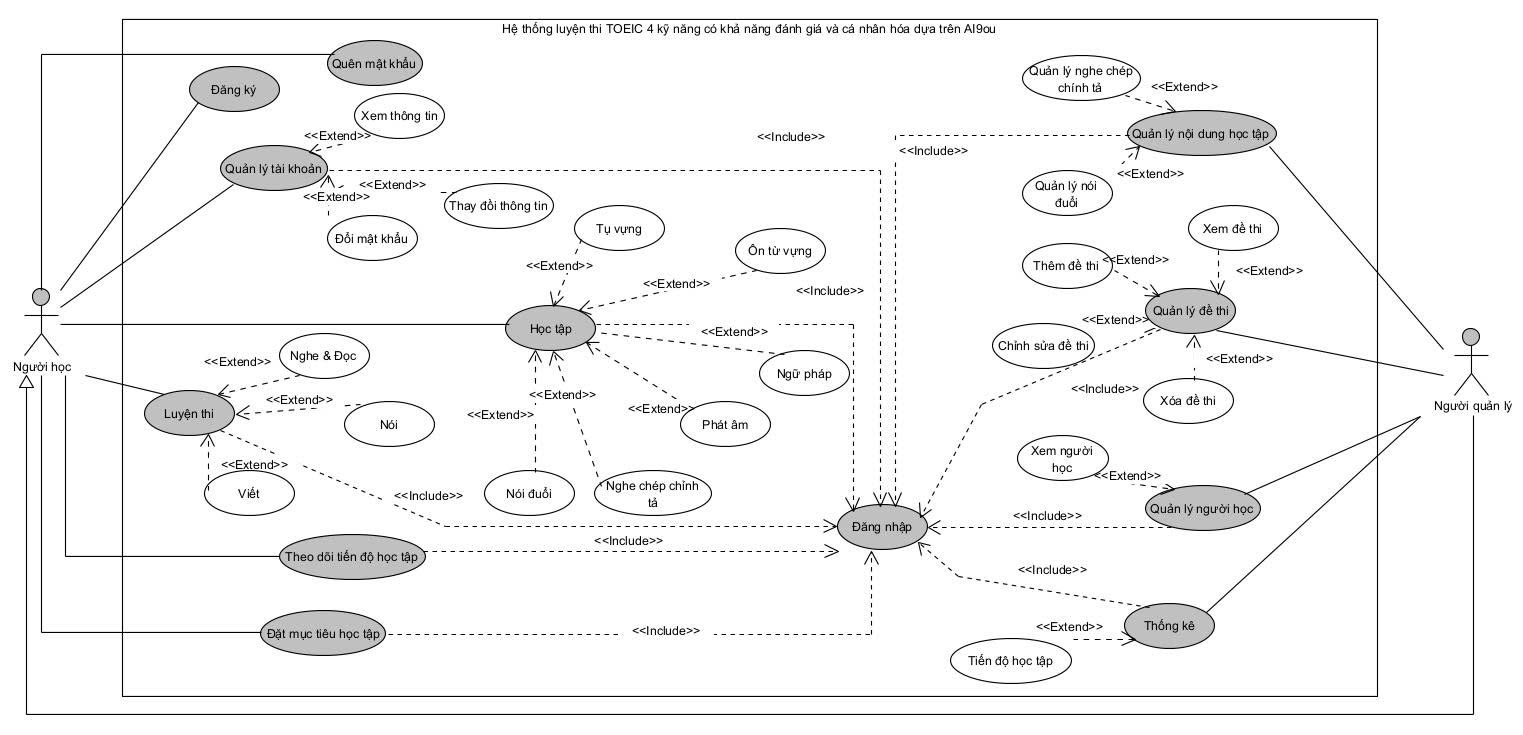
\includegraphics[width=0.8\linewidth]{use-case.jpg} 
    
    \caption{Sơ đồ use-case} % Ví dụ: Sơ đồ Use-case tổng quát
    \label{fig:ten-goi-nho-0} % Dùng để trích dẫn (VD: Hình \ref{fig:ten-goi-nho})
\end{figure}

\section{Danh sách tác nhân và mô tả}

Hệ thống có hai tác nhân chính tương tác trực tiếp:

\begin{table}[!ht]
    \centering
    \renewcommand{\arraystretch}{1.3}
    \begin{tabularx}{\linewidth}{|l|X|}
        \hline
        \textbf{Tác nhân} & \textbf{Mô tả} \\ \hline
        Người học (Learner) & Người dùng cuối đã đăng ký tài khoản. Người học sử dụng hệ thống để thực hiện kiểm tra đầu vào, học từ vựng, ngữ pháp, luyện 4 kỹ năng IELTS, thi thử Mock Test và theo dõi tiến độ học tập cá nhân. \\ \hline
        Người quản lý (Admin) & Người có quyền quản trị hệ thống. Admin chịu trách nhiệm tạo và quản lý toàn bộ nội dung học tập (từ vựng, ngữ pháp, bài nghe, bài đọc, đề Writing, đề Speaking, đề thi Mock Test), quản lý tài khoản học viên và theo dõi báo cáo thống kê hoạt động hệ thống. \\ \hline
    \end{tabularx}
    \caption{Danh sách tác nhân và mô tả}
    \label{tab:actors}
\end{table}

\section{Danh sách các tình huống hoạt động chính}

\renewcommand{\arraystretch}{1.2}
\begin{longtable}{|p{1.5cm}|p{4.5cm}|p{8.0cm}|}
    \caption{Danh sách các tình huống hoạt động chính}
    \label{tab:uc_list} \\
    \hline
    \textbf{Mã UC} & \textbf{Tên use case} & \textbf{Mô tả ngắn} \\ \hline
    \endfirsthead
    \multicolumn{3}{r}{\textit{(tiếp trang trước)}} \\
    \hline
    \textbf{Mã UC} & \textbf{Tên use case} & \textbf{Mô tả ngắn} \\ \hline
    \endhead
    \hline \multicolumn{3}{r}{\textit{(tiếp trang sau)}} \\
    \endfoot
    \hline
    \endlastfoot
    UC01 & Đăng ký tài khoản & Người học tạo tài khoản mới bằng email và xác thực danh tính qua mã OTP. \\ \hline
    UC02 & Đăng nhập & Người học đăng nhập vào hệ thống; tài khoản bị khóa 15 phút sau 5 lần sai liên tiếp. \\ \hline
    UC03 & Kiểm tra đầu vào & Người học hoàn thành Placement Test để xác định trình độ CEFR và nhận lộ trình học đề xuất. \\ \hline
    UC04 & Học từ vựng & Người học học từ vựng theo đơn vị (unit), trả lời câu hỏi ôn tập và đọc hiểu cuối unit. \\ \hline
    UC05 & Ôn từ vựng & Người học ôn từ vựng đã lưu bằng Flashcard với thuật toán Spaced Repetition (SM-2). \\ \hline
    UC06 & Học ngữ pháp & Người học học lý thuyết ngữ pháp theo unit và hoàn thành bài tập thực hành. \\ \hline
    UC07 & Luyện phát âm & Người học nghe phát âm chuẩn, thu âm và nhận đánh giá AI về độ chính xác từng âm vị. \\ \hline
    UC08 & Luyện Listening & Người học nghe audio và nhập transcript (Dictation); nhận phản hồi chi tiết theo loại lỗi. \\ \hline
    UC09 & Luyện Reading & Người học đọc đoạn văn IELTS Academic và trả lời các dạng câu hỏi đọc hiểu. \\ \hline
    UC10 & Luyện Writing Task 1 & Người học viết mô tả biểu đồ/quy trình; nhận band điểm và nhận xét tự động từ AI. \\ \hline
    UC11 & Luyện Writing Task 2 & Người học viết bài luận IELTS; nhận band điểm theo 4 tiêu chí và gợi ý cải thiện từ AI. \\ \hline
    UC12 & Luyện Speaking -- Shadowing & Người học nói đuổi theo audio mẫu; hệ thống đánh giá phát âm và nhịp điệu bằng AI. \\ \hline
    UC13 & Luyện Speaking -- AI Conversation & Người học hội thoại với AI theo chủ đề IELTS Part 1/2/3; nhận phản hồi về kỹ năng Speaking. \\ \hline
    UC14 & Thi thử IELTS (Mock Test) & Người học thi thử IELTS toàn phần hoặc theo kỹ năng; nhận kết quả và band điểm ước tính. \\ \hline
    UC15 & Xem kết quả và phân tích lỗi & Người học xem lại kết quả bài làm, đáp án và phân tích lỗi chi tiết theo từng câu. \\ \hline
    UC16 & Đặt mục tiêu học tập & Người học thiết lập band điểm mục tiêu, thời hạn và kế hoạch học hàng ngày. \\ \hline
    UC17 & Xem tiến độ học tập & Người học theo dõi tiến độ qua biểu đồ thống kê theo kỹ năng và theo thời gian. \\ \hline
    UC18 & Quản lý nội dung học tập & Admin tạo, chỉnh sửa và xuất bản học liệu cho tất cả các kỹ năng. \\ \hline
    UC19 & Quản lý đề thi & Admin xây dựng ngân hàng câu hỏi và cấu trúc đề Mock Test chuẩn IELTS. \\ \hline
    UC20 & Quản lý học viên & Admin xem hồ sơ, tiến độ và quản lý trạng thái tài khoản học viên. \\ \hline
    UC21 & Xem thống kê báo cáo & Admin xem các chỉ số hệ thống: DAU, tỷ lệ hoàn thành bài, phổ band điểm. \\ \hline
\end{longtable}

\section{Đặc tả các yêu cầu chức năng}

Trong phần này, chúng em trình bày đặc tả chi tiết cho các use case quan trọng nhất. Mỗi use case bao gồm bảng mô tả luồng sự kiện (chính và thay thế), sơ đồ activity và mô tả kỹ thuật chi tiết.

\subsection{Đăng ký tài khoản (UC01)}
\subsubsection{Mô tả use case}
\begin{table}[!ht]
    \centering
    \renewcommand{\arraystretch}{1.1}
    \begin{tabularx}{\linewidth}{|X|X|}
        \hline
        \multicolumn{2}{|l|}{\textbf{Đặc tả use case}} \\ \hline
        \multicolumn{2}{|l|}{\textbf{Mã use case:} UC01} \\ \hline
        \multicolumn{2}{|l|}{\textbf{Actor:} Người học} \\ \hline
        \multicolumn{2}{|p{\dimexpr\linewidth-2\tabcolsep-2\arrayrulewidth}|}{\textbf{Tiền điều kiện (Pre-condition):} Người dùng chưa có tài khoản và truy cập trang đăng ký.} \\ \hline
        \multicolumn{2}{|p{\dimexpr\linewidth-2\tabcolsep-2\arrayrulewidth}|}{\textbf{Hậu điều kiện (Post-condition):} Tài khoản được tạo thành công; hệ thống chuyển người dùng đến màn hình Kiểm tra đầu vào (Placement Test).} \\ \hline
        \multicolumn{2}{|l|}{\textbf{Luồng sự kiện chính (Basic Flow)}} \\ \hline
        \textbf{Tác nhân} & \textbf{Hệ thống} \\ \hline

        1. Người học nhập địa chỉ email và mật khẩu (tối thiểu 8 ký tự), sau đó chọn "Đăng ký". & \\ \hline

        & 2. Hệ thống kiểm tra định dạng email hợp lệ và xác nhận email chưa tồn tại trong cơ sở dữ liệu. \\ \hline

        & 3. Hệ thống tạo mã OTP 6 chữ số với thời hạn 5 phút và gửi đến địa chỉ email của người học. \\ \hline

        4. Người học kiểm tra hộp thư điện tử và nhập mã OTP vào ô xác thực. & \\ \hline

        & 5. Hệ thống xác thực mã OTP còn hiệu lực và khớp với mã đã gửi. \\ \hline

        & 6. Hệ thống mã hóa mật khẩu bằng thuật toán bcrypt (salt rounds = 12) và tạo bản ghi người dùng trong Supabase Auth. \\ \hline

        & 7. Hệ thống cấp cặp token (access token hiệu lực 15 phút, refresh token hiệu lực 7 ngày) và chuyển hướng người học đến màn hình Placement Test. \\ \hline

        \multicolumn{2}{|l|}{\textbf{Luồng sự kiện thay thế (Alternative Flow)}} \\ \hline

        & 2a. Email đã được đăng ký: hệ thống hiển thị thông báo "Email đã tồn tại, vui lòng đăng nhập" và dừng luồng. \\ \hline

        & 2b. Mật khẩu dưới 8 ký tự: hệ thống hiển thị thông báo yêu cầu và dừng luồng. \\ \hline

        & 5a. Mã OTP sai hoặc hết hạn: hệ thống hiển thị thông báo lỗi và cho phép nhập lại hoặc yêu cầu gửi lại OTP (tối đa 3 lần mỗi giờ). \\ \hline

    \end{tabularx}
    \caption{Đặc tả Use-case Đăng ký tài khoản (UC01)}
    \label{tab:uc01_spec}
\end{table}

\subsubsection{Sơ đồ activity}
\begin{figure}[H]
    \centering
    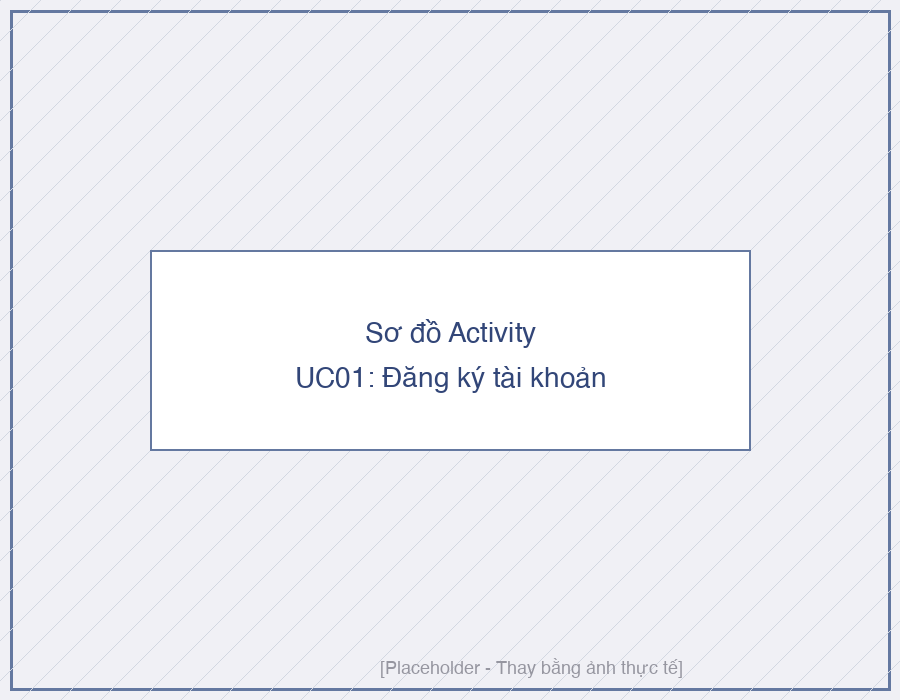
\includegraphics[width=0.85\linewidth]{activity-uc01.png}
    \caption{Sơ đồ activity UC01 -- Đăng ký tài khoản}
    \label{fig:activity-uc01}
\end{figure}

\subsubsection{Mô tả kỹ thuật chi tiết}

Điểm kỹ thuật quan trọng nhất trong UC01 là cơ chế bảo mật tại bước tạo tài khoản. Mật khẩu của người học không bao giờ được lưu dưới dạng plain text. Thay vào đó, NestJS Authentication Service gọi hàm \texttt{bcrypt.hash(password, 12)} để tạo hash cùng salt 12 vòng -- con số này đảm bảo mỗi lần hash mất khoảng 300--500ms, đủ chậm để chống tấn công brute-force nhưng không ảnh hưởng đến trải nghiệm đăng ký.

Hệ thống OTP được triển khai phía NestJS với luồng sau: khi nhận yêu cầu đăng ký, User Service tạo mã ngẫu nhiên 6 chữ số, lưu vào bảng \texttt{otp\_tokens} trong PostgreSQL cùng với trường \texttt{expires\_at = now() + 5 phút} và \texttt{attempts = 0}. Sau đó, hệ thống gọi Supabase SMTP để gửi email. Tại bước xác thực, User Service kiểm tra đồng thời ba điều kiện: OTP khớp, \texttt{expires\_at} chưa qua và \texttt{attempts < 3}; mỗi lần nhập sai, trường \texttt{attempts} tăng thêm 1. Cơ chế này ngăn tấn công brute-force OTP hiệu quả.

\begin{sloppypar}
Sau khi xác thực thành công, hệ thống gọi Supabase Auth \texttt{signUp()} API để tạo bản ghi xác thực, đồng thời NestJS User Service tạo bản ghi trong bảng \texttt{users} với quan hệ 1-1 dựa trên \texttt{user\_id} từ Supabase Auth. JWT được phát hành theo cặp: access token (payload: \texttt{sub, email, role}; TTL 15 phút) và refresh token (TTL 7 ngày, lưu trong HttpOnly cookie để chống XSS).
\end{sloppypar}

\subsection{Đăng nhập (UC02)}
\subsubsection{Mô tả use case}
\begin{table}[!ht]
    \centering
    \renewcommand{\arraystretch}{1.1}
    \begin{tabularx}{\linewidth}{|X|X|}
        \hline
        \multicolumn{2}{|l|}{\textbf{Đặc tả use case}} \\ \hline
        \multicolumn{2}{|l|}{\textbf{Mã use case:} UC02} \\ \hline
        \multicolumn{2}{|l|}{\textbf{Actor:} Người học} \\ \hline
        \multicolumn{2}{|p{\dimexpr\linewidth-2\tabcolsep-2\arrayrulewidth}|}{\textbf{Tiền điều kiện (Pre-condition):} Người học đã có tài khoản được xác thực email.} \\ \hline
        \multicolumn{2}{|p{\dimexpr\linewidth-2\tabcolsep-2\arrayrulewidth}|}{\textbf{Hậu điều kiện (Post-condition):} Người học truy cập thành công vào Dashboard; hệ thống lưu trạng thái phiên làm việc.} \\ \hline
        \multicolumn{2}{|l|}{\textbf{Luồng sự kiện chính (Basic Flow)}} \\ \hline
        \textbf{Tác nhân} & \textbf{Hệ thống} \\ \hline

        1. Người học nhập địa chỉ email và mật khẩu, sau đó chọn "Đăng nhập". & \\ \hline

        & 2. Hệ thống kiểm tra trạng thái khóa tài khoản; nếu chưa bị khóa, tiếp tục xử lý. \\ \hline

        & 3. Hệ thống truy vấn cơ sở dữ liệu bằng email, gọi \texttt{bcrypt.compare()} để so sánh mật khẩu nhập vào với hash đã lưu. \\ \hline

        & 4. Hệ thống đặt lại bộ đếm thất bại về 0, tạo JWT access token (15 phút) và refresh token (7 ngày). \\ \hline

        & 5. Hệ thống lưu refresh token vào HttpOnly cookie và chuyển hướng người học đến màn hình Dashboard. \\ \hline

        \multicolumn{2}{|l|}{\textbf{Luồng sự kiện thay thế (Alternative Flow)}} \\ \hline

        & 3a. Email không tồn tại hoặc mật khẩu sai: hệ thống tăng bộ đếm thất bại thêm 1 và hiển thị thông báo "Email hoặc mật khẩu không đúng". \\ \hline

        & 3b. Bộ đếm đạt 5 lần liên tiếp trong 15 phút: hệ thống khóa tài khoản và hiển thị "Tài khoản tạm thời bị khóa, vui lòng thử lại sau 15 phút". \\ \hline

        & 2a. Tài khoản đang bị khóa: hiển thị thời gian còn lại đến khi mở khóa và dừng luồng. \\ \hline

        & (Token hết hạn): Client tự động gửi refresh token để nhận cặp token mới mà không yêu cầu người học đăng nhập lại (silent refresh). \\ \hline

    \end{tabularx}
    \caption{Đặc tả Use-case Đăng nhập (UC02)}
    \label{tab:uc02_spec}
\end{table}

\subsubsection{Sơ đồ activity}
\begin{figure}[H]
    \centering
    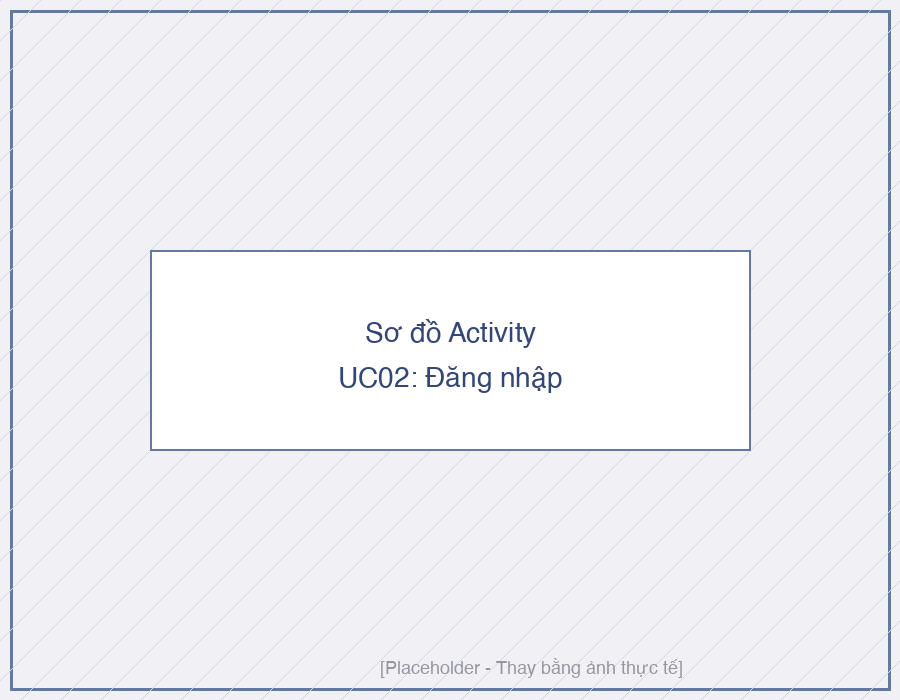
\includegraphics[width=0.85\linewidth]{activity-uc02.png}
    \caption{Sơ đồ activity UC02 -- Đăng nhập}
    \label{fig:activity-uc02}
\end{figure}

\subsubsection{Mô tả kỹ thuật chi tiết}

Cơ chế bảo vệ chống brute-force trong UC02 được triển khai theo mô hình sliding window với hai thông số: số lần thất bại tối đa (\texttt{MAX\_ATTEMPTS = 5}) và cửa sổ thời gian (\texttt{WINDOW = 15 phút}). Mỗi tài khoản có hai trường trong bảng \texttt{users}: \texttt{failed\_attempts} và \texttt{lock\_until}. Khi người học đăng nhập sai, User Service tăng \texttt{failed\_attempts}; nếu đạt ngưỡng 5, hệ thống ghi \texttt{lock\_until = now() + 15 phút}. Tại mỗi lần đăng nhập mới, hệ thống kiểm tra \texttt{lock\_until > now()} trước tiên -- nếu đúng, từ chối xử lý ngay mà không cần truy vấn password.

Điểm kỹ thuật quan trọng trong bước so sánh mật khẩu là hàm \texttt{bcrypt.compare()} sử dụng constant-time comparison -- thời gian thực thi không phụ thuộc vào vị trí ký tự đầu tiên sai, giúp ngăn timing attack. Kết quả boolean từ hàm này được dùng trực tiếp mà không có logic rẽ nhánh sớm.

\begin{sloppypar}
Cơ chế JWT rotation bảo vệ phiên làm việc dài hạn: khi access token hết hạn, client gửi refresh token (lưu trong HttpOnly cookie) đến endpoint \texttt{POST /auth/refresh}. API Gateway xác thực chữ ký JWT của refresh token, sau đó User Service cấp cặp token hoàn toàn mới và vô hiệu hóa refresh token cũ trong bảng \texttt{refresh\_tokens}. Cơ chế này đảm bảo nếu refresh token bị đánh cắp, kẻ tấn công chỉ sử dụng được một lần trước khi bị phát hiện.
\end{sloppypar}

\subsection{Học từ vựng (UC04)}
\subsubsection{Mô tả use case}
\begin{table}[!ht]
    \centering
    \renewcommand{\arraystretch}{1.1} % Tăng chiều cao dòng cho dễ đọc
    % Định nghĩa bảng: Chiều rộng bằng dòng chữ, có 2 cột bằng nhau (X)
    \begin{tabularx}{\linewidth}{|X|X|}
        \hline
        \multicolumn{2}{|l|}{\textbf{Đặc tả use case}} \\ \hline
        \multicolumn{2}{|l|}{\textbf{Mã use case:} UC04} \\ \hline
        \multicolumn{2}{|l|}{\textbf{Actor:} Người học} \\ \hline
        \multicolumn{2}{|p{\dimexpr\linewidth-2\tabcolsep-2\arrayrulewidth}|}{\textbf{Tiền điều kiện (Pre-condition):} Người học đã đăng nhập thành công vào hệ thống.} \\ \hline
        \multicolumn{2}{|p{\dimexpr\linewidth-2\tabcolsep-2\arrayrulewidth}|}{\textbf{Hậu điều kiện (Post-condition):} Hệ thống ghi nhận và hiển thị trạng thái hoàn thành của unit tương ứng.} \\ \hline
        \multicolumn{2}{|l|}{\textbf{Luồng sự kiện chính (Basic Flow)}} \\ \hline
        \textbf{Tác nhân} & \textbf{Hệ thống} \\ \hline
        
        1. Người học lựa chọn một đơn vị bài học (unit). & \\ \hline
        
        & 2. Hệ thống hiển thị danh sách từ vựng unit theo thứ tự, mỗi từ bao gồm: từ vựng, nghĩa, câu ví dụ minh họa và phát âm. \\ \hline
        
        3. Người học đọc, nghe phát âm, chọn từ tiếp theo hoặc thêm từ vựng vào mục ôn từ vựng và chọn hoàn thành. & \\ \hline
        
        & 4. Hệ thống hiển thị các câu hỏi ôn tập tương ứng, lần lượt từng câu một. \\ \hline
        
        5. Người học trả lời các câu hỏi và nộp bài. & \\ \hline
        
        & 6. Hệ thống kiểm tra kết quả và hiển thị đáp án. \\ \hline
        
        7. Người học xem lại kết quả và chọn tiếp tục. & \\ \hline
        
        & 8. Hệ thống hiển thị một đoạn văn chứa các từ vựng vừa học, kèm theo tệp âm thanh và các câu hỏi đọc hiểu. \\ \hline
        
        9. Người học đọc đoạn văn, trả lời câu hỏi hoặc thêm từ vựng vào mục ôn từ vựng và nộp bài. & \\ \hline
        
        & 10. Hệ thống kiểm tra kết quả và hiển thị đáp án cho phần đọc hiểu. \\ \hline
        
        11. Người dùng xem và chọn hoàn thành. & \\ \hline
        
        & 12. Hệ thống cập nhật trạng thái hoàn thành và chuyển người học trở về màn hình chính học từ vựng. \\ \hline
        
        \multicolumn{2}{|l|}{\textbf{Luồng sự kiện thay thế (Alternative Flow)}} \\ \hline
        
        & 6. Hiển thị đáp án không hợp lệ và quay lại bước 4. \\ \hline
        
        & 10. Hiển thị đáp án không hợp lệ và quay lại bước 8. \\ \hline
        
    \end{tabularx}
    \caption{Đặc tả Use-case Học từ vựng (UC04)}
    \label{tab:uc04_spec}
\end{table}
\subsubsection{Sơ đồ activity}
\begin{figure}[H]
    \centering
    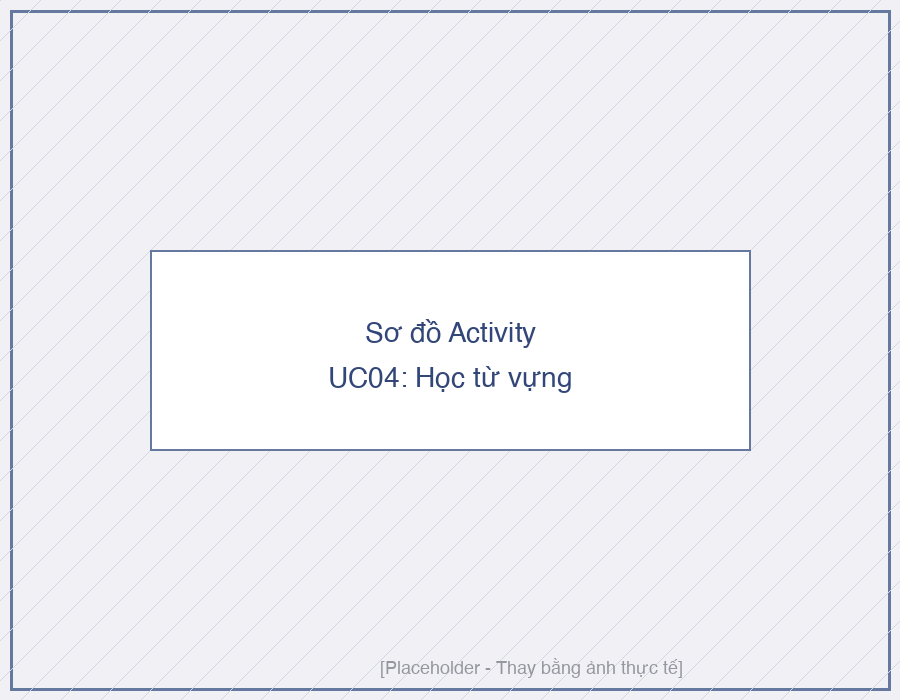
\includegraphics[width=0.85\linewidth]{activity-uc04.png}
    \caption{Sơ đồ activity UC04 -- Học từ vựng}
    \label{fig:activity-uc04}
\end{figure}

\subsection{Ôn từ vựng (UC05)}
\subsubsection{Mô tả use case}
\begin{table}[!ht]
    \centering
    \renewcommand{\arraystretch}{1.1} % Tăng khoảng cách dòng
    % Tạo bảng với 2 cột rộng bằng nhau (X), tổng chiều rộng bằng trang giấy
    \begin{tabularx}{\linewidth}{|X|X|}
        \hline
        \multicolumn{2}{|l|}{\textbf{Đặc tả use case}} \\ \hline
        \multicolumn{2}{|l|}{\textbf{Mã use case:} UC05} \\ \hline
        \multicolumn{2}{|l|}{\textbf{Actor:} Người học} \\ \hline
        \multicolumn{2}{|p{\dimexpr\linewidth-2\tabcolsep-2\arrayrulewidth}|}{\textbf{Tiền điều kiện (Pre-condition):} Người học đã đăng nhập thành công vào hệ thống.} \\ \hline
        \multicolumn{2}{|p{\dimexpr\linewidth-2\tabcolsep-2\arrayrulewidth}|}{\textbf{Hậu điều kiện (Post-condition):} Hệ thống ghi nhận trạng thái hoàn thành của bộ thẻ (deck) và cập nhật tiến độ ôn tập của người học.} \\ \hline
        \multicolumn{2}{|l|}{\textbf{Luồng sự kiện chính (Basic Flow)}} \\ \hline
        \textbf{Tác nhân} & \textbf{Hệ thống} \\ \hline
        
        1. Người học chọn chức năng “Ôn từ vựng”. & \\ \hline
        
        & 2. Hệ thống hiển thị danh sách các deck có sẵn để ôn tập. \\ \hline
        
        3. Người học chọn một deck cần ôn. & \\ \hline
        
        & 4. Hệ thống kiểm tra xem trong deck còn thẻ (card) chưa ôn hay không. Nếu còn, hệ thống hiển thị mặt trước của thẻ tiếp theo (gồm từ vựng cần ôn). \\ \hline
        
        5. Người học cố gắng ghi nhớ nghĩa và chọn “Hiển thị đáp án”. & \\ \hline
        
        & 6. Hệ thống hiển thị mặt sau của thẻ (nghĩa, ví dụ, phát âm) và bốn lựa chọn: “Again”, “Hard”, “Good”, “Easy”. \\ \hline
        
        7. Người học chọn một trong bốn lựa chọn. & \\ \hline
        
        & 8. Hệ thống ghi nhận lựa chọn của người học, tính toán thời điểm xuất hiện lại của thẻ theo thuật toán lặp lại ngắt quãng, sau đó hiển thị thẻ tiếp theo. \\ \hline
        
        & 9. Khi toàn bộ các thẻ trong deck đã được ôn, hệ thống thông báo hoàn thành và chuyển người học về màn hình chính. \\ \hline
        
        \multicolumn{2}{|l|}{\textbf{Luồng sự kiện ngoại lệ (Alternative Flow)}} \\ \hline
        
        % (Để trống vì trong hình không hiển thị nội dung phần này)
        & \\ \hline

    \end{tabularx}
    \caption{Đặc tả Use-case Ôn từ vựng (UC05)}
    \label{tab:uc05_spec}
\end{table}
\subsubsection{Sơ đồ activity}
\begin{figure}[H]
    \centering
    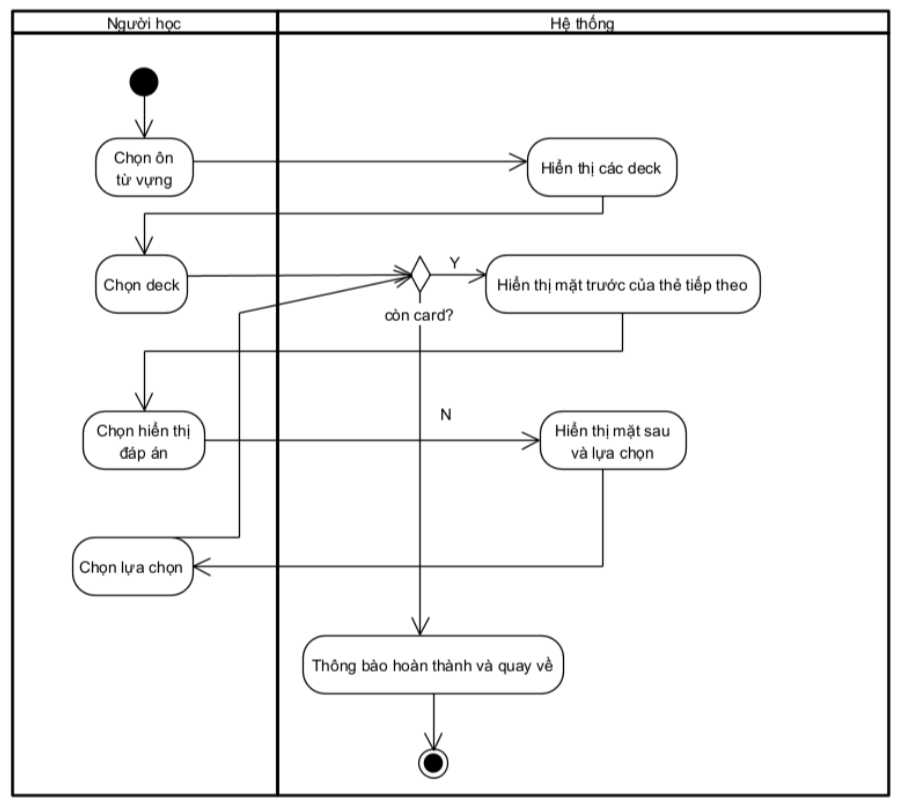
\includegraphics[width=0.8\linewidth]{on-tu-activity.png} 
    
    \caption{Sơ đồ activity UC05 -- Ôn từ vựng}
    \label{fig:activity-uc05}
\end{figure}

\subsection{Luyện Listening (UC08)}
\subsubsection{Mô tả use case}
\begin{table}[!ht]
    \centering
    \renewcommand{\arraystretch}{1.1}
    \begin{tabularx}{\linewidth}{|X|X|}
        \hline
        \multicolumn{2}{|l|}{\textbf{Đặc tả use case}} \\ \hline
        \multicolumn{2}{|l|}{\textbf{Mã use case:} UC08} \\ \hline
        \multicolumn{2}{|l|}{\textbf{Actor:} Người học} \\ \hline
        \multicolumn{2}{|p{\dimexpr\linewidth-2\tabcolsep-2\arrayrulewidth}|}{\textbf{Tiền điều kiện (Pre-condition):} Người học đã đăng nhập và chọn một bài luyện Listening từ hệ thống.} \\ \hline
        \multicolumn{2}{|p{\dimexpr\linewidth-2\tabcolsep-2\arrayrulewidth}|}{\textbf{Hậu điều kiện (Post-condition):} Hệ thống ghi nhận kết quả bài làm, lưu lịch sử luyện tập và hiển thị phân tích lỗi chi tiết.} \\ \hline
        \multicolumn{2}{|l|}{\textbf{Luồng sự kiện chính (Basic Flow)}} \\ \hline
        \textbf{Tác nhân} & \textbf{Hệ thống} \\ \hline

        1. Người học chọn bài luyện Listening theo chủ đề hoặc dạng đề. & \\ \hline

        & 2. Hệ thống tải audio từ Supabase Storage và hiển thị danh sách câu hỏi Dictation (điền vào chỗ trống theo những gì nghe được). \\ \hline

        3. Người học nhấn phát, nghe audio và nhập câu trả lời vào các ô điền tương ứng. Người học có thể tua lại và phát lại nhiều lần. & \\ \hline

        4. Người học hoàn tất và nộp bài. & \\ \hline

        & 5. Hệ thống chuẩn hóa văn bản nhập vào (chuyển thường, loại bỏ dấu câu thừa) và so sánh với đáp án chuẩn theo từng ô. \\ \hline

        & 6. Hệ thống phân loại kết quả từng ô: Đúng hoàn toàn, Gần đúng (khoảng cách Levenshtein $\leq$ 1) hoặc Sai. Tính điểm và phân tích loại lỗi (sai từ, thiếu từ, thêm từ). \\ \hline

        & 7. Hệ thống hiển thị bảng kết quả: tỉ lệ đúng, điểm số, từng câu kèm đáp án đúng và phân loại lỗi (màu xanh/đỏ). \\ \hline

        \multicolumn{2}{|l|}{\textbf{Luồng sự kiện thay thế (Alternative Flow)}} \\ \hline

        & 2a. Không thể tải audio (lỗi mạng): hệ thống thử lại tối đa 3 lần; nếu vẫn thất bại, hiển thị thông báo lỗi và cho phép chọn bài khác. \\ \hline

        & 4a. Người học nộp khi còn ô trống: hệ thống cảnh báo số ô chưa điền và cho phép tiếp tục hoặc nộp thẳng. \\ \hline

    \end{tabularx}
    \caption{Đặc tả Use-case Luyện Listening (UC08)}
    \label{tab:uc08_spec}
\end{table}

\subsubsection{Sơ đồ activity}
\begin{figure}[H]
    \centering
    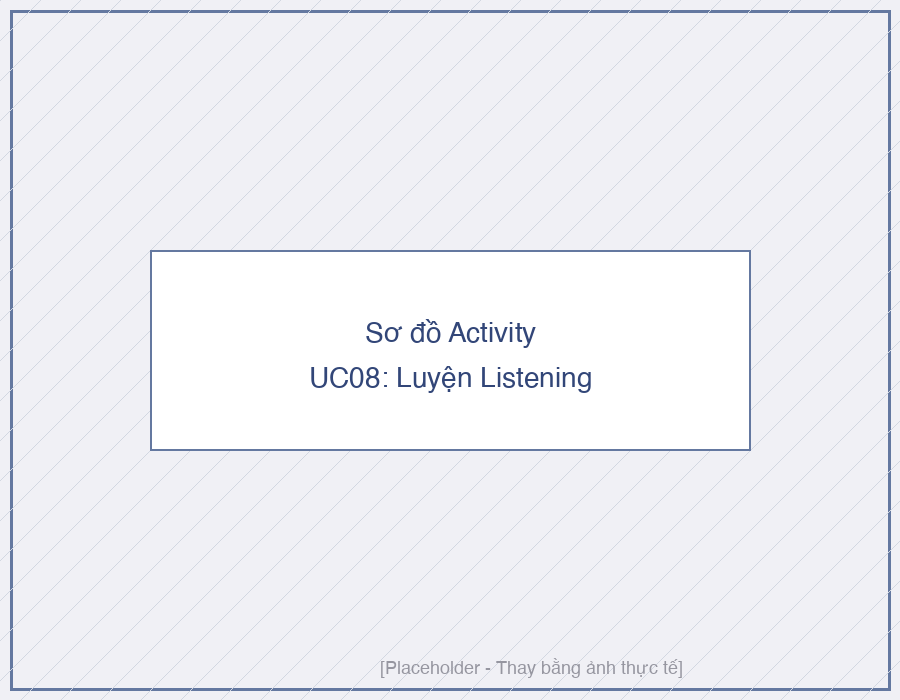
\includegraphics[width=0.85\linewidth]{activity-uc08.png}
    \caption{Sơ đồ activity UC08 -- Luyện Listening}
    \label{fig:activity-uc08}
\end{figure}

\subsubsection{Mô tả kỹ thuật chi tiết}

Tính năng Luyện Listening tập trung vào dạng bài Dictation -- người học nghe và điền từ còn thiếu -- mô phỏng sát dạng câu hỏi điền từ phổ biến trong IELTS Listening. Audio được lưu trên Supabase Storage với đường dẫn CDN công khai, trình duyệt phát trực tiếp qua thẻ HTML5 \texttt{<audio>} (trên web) hoặc đối tượng \texttt{expo-av} Audio (trên mobile), cho phép tua ngẫu nhiên và điều chỉnh tốc độ phát.

Điểm kỹ thuật quan trọng nhất là thuật toán chấm điểm linh hoạt tại bước 5--6. Sau khi nhận câu trả lời, Assessment Service thực hiện ba bước xử lý: (1) \textit{Chuẩn hóa:} chuyển toàn bộ về chữ thường, loại bỏ ký tự dấu câu không cần thiết (\texttt{.,!?}), trim khoảng trắng thừa; (2) \textit{Tokenize:} tách chuỗi thành mảng từ; (3) \textit{So sánh:} với từng cặp (từ người học, từ đáp án), tính khoảng cách Levenshtein -- nếu khoảng cách $\leq$ 1 và độ dài từ $\geq$ 5, đánh dấu "gần đúng" (vẫn tính điểm đầy đủ). Ngưỡng này bỏ qua lỗi chính tả nhỏ không ảnh hưởng đến nghĩa, phản ánh đúng tinh thần chấm điểm IELTS Listening.

Kết quả được phân loại thành ba loại lỗi: \textbf{Wrong Word} (từ sai hoàn toàn), \textbf{Missing Word} (người học bỏ trống) và \textbf{Extra Word} (người học điền thêm từ không có trong đáp án). Phân loại này giúp người học nhận ra điểm yếu cụ thể: lỗi Missing Word liên tục gợi ý người học nghe không kịp tốc độ, còn lỗi Wrong Word gợi ý cần cải thiện phân biệt âm vị (phoneme discrimination).

\subsection{Luyện Writing Task 2 (UC11)}
\subsubsection{Mô tả use case}
\begin{table}[!ht]
    \centering
    \renewcommand{\arraystretch}{1.1}
    \begin{tabularx}{\linewidth}{|X|X|}
        \hline
        \multicolumn{2}{|l|}{\textbf{Đặc tả use case}} \\ \hline
        \multicolumn{2}{|l|}{\textbf{Mã use case:} UC11} \\ \hline
        \multicolumn{2}{|l|}{\textbf{Actor:} Người học} \\ \hline
        \multicolumn{2}{|p{\dimexpr\linewidth-2\tabcolsep-2\arrayrulewidth}|}{\textbf{Tiền điều kiện (Pre-condition):} Người học đã đăng nhập và chọn một đề Writing Task 2.} \\ \hline
        \multicolumn{2}{|p{\dimexpr\linewidth-2\tabcolsep-2\arrayrulewidth}|}{\textbf{Hậu điều kiện (Post-condition):} Hệ thống lưu bài viết, hiển thị band điểm theo 4 tiêu chí IELTS Writing và gợi ý cải thiện chi tiết.} \\ \hline
        \multicolumn{2}{|l|}{\textbf{Luồng sự kiện chính (Basic Flow)}} \\ \hline
        \textbf{Tác nhân} & \textbf{Hệ thống} \\ \hline

        1. Người học chọn đề Writing Task 2 và chọn "Bắt đầu làm bài". & \\ \hline

        & 2. Hệ thống hiển thị đề bài (chủ đề, thể loại bài luận) cùng editor soạn thảo và bộ đếm từ real-time. \\ \hline

        3. Người học viết bài luận trong editor. Bộ đếm từ cập nhật liên tục khi người học gõ. & \\ \hline

        4. Người học hoàn thành và chọn "Nộp bài". & \\ \hline

        & 5. Hệ thống lưu bài viết vào cơ sở dữ liệu và gửi yêu cầu chấm điểm đến Assessment Service. \\ \hline

        & 6. Assessment Service xây dựng prompt và gửi đến Gemini API (\texttt{gemini-1.5-flash}): prompt chứa đề bài, bài viết của người học và JSON schema kết quả mong muốn. \\ \hline

        & 7. Gemini API phân tích bài viết theo 4 tiêu chí IELTS Writing Task 2 và trả về JSON: band từng tiêu chí, band tổng, nhận xét tổng quan, danh sách điểm mạnh và điểm cần cải thiện. \\ \hline

        & 8. Hệ thống hiển thị kết quả: band điểm từng tiêu chí (TA, CC, LR, GRA), band tổng ước tính và nhận xét chi tiết kèm ví dụ cụ thể từ bài viết. \\ \hline

        \multicolumn{2}{|l|}{\textbf{Luồng sự kiện thay thế (Alternative Flow)}} \\ \hline

        & 4a. Bài viết dưới 250 từ: hệ thống cảnh báo "Bài viết cần ít nhất 250 từ để đạt điểm tối đa" nhưng vẫn cho phép nộp. \\ \hline

        & 7a. Gemini API không phản hồi sau 30 giây: hệ thống thử lại một lần; nếu vẫn thất bại, hiển thị "Dịch vụ chấm điểm đang bận, vui lòng thử lại sau". \\ \hline

    \end{tabularx}
    \caption{Đặc tả Use-case Luyện Writing Task 2 (UC11)}
    \label{tab:uc11_spec}
\end{table}

\subsubsection{Sơ đồ activity}
\begin{figure}[H]
    \centering
    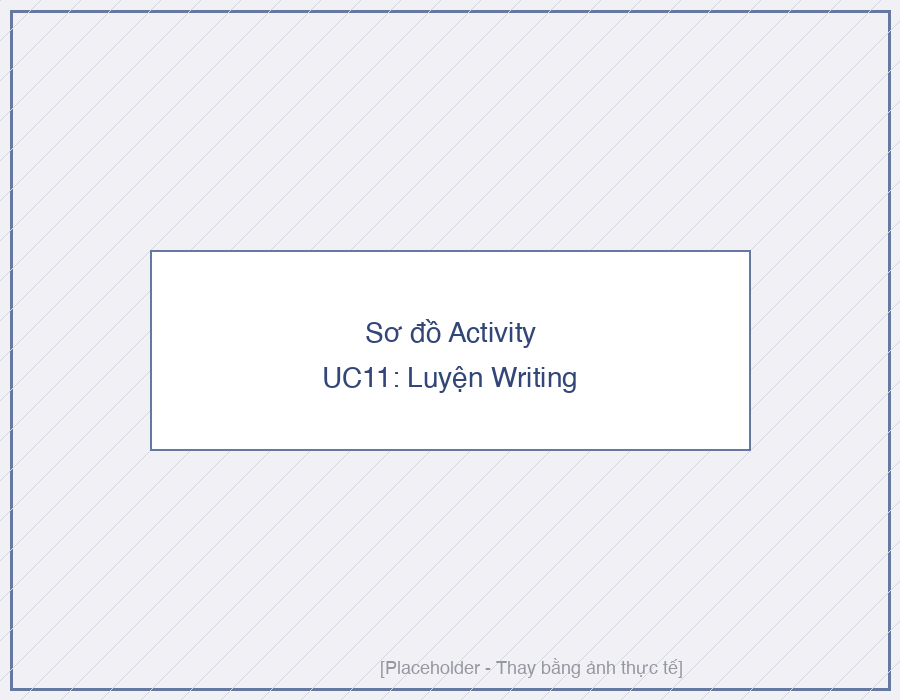
\includegraphics[width=0.85\linewidth]{activity-uc11.png}
    \caption{Sơ đồ activity UC11 -- Luyện Writing Task 2}
    \label{fig:activity-uc11}
\end{figure}

\subsubsection{Mô tả kỹ thuật chi tiết}

Cơ chế chấm điểm Writing Task 2 dựa hoàn toàn vào Gemini API với kỹ thuật \textit{prompt engineering} và \textit{structured output}. Cụ thể, Assessment Service xây dựng prompt theo ba phần: (1) \textit{System instruction:} định nghĩa vai trò của Gemini là giám khảo IELTS chuyên nghiệp, hiểu rõ rubric chính thức và chỉ trả về JSON theo schema quy định; (2) \textit{Essay context:} đề bài Writing Task 2 và loại bài luận (opinion, discussion, problem-solution, direct question); (3) \textit{Essay text:} nội dung bài viết của người học nguyên vẹn.

Để đảm bảo Gemini trả về đúng cấu trúc dữ liệu, hệ thống sử dụng tham số \texttt{responseSchema} của Gemini API. Schema bắt buộc gồm: \texttt{band\_ta} (float), \texttt{band\_cc} (float), \texttt{band\_lr} (float), \texttt{band\_gra} (float), \texttt{overall\_band} (float), \texttt{overview} (string), \texttt{strengths} (mảng string) và \texttt{improvements} (mảng object gồm category, issue, example, suggestion).

Bốn tiêu chí chấm điểm tương ứng với 4 tiêu chí IELTS Writing chính thức: \textbf{Task Achievement (TA)} -- mức độ đáp ứng yêu cầu đề bài và phát triển luận điểm; \textbf{Coherence and Cohesion (CC)} -- tính liên kết giữa các đoạn và câu; \textbf{Lexical Resource (LR)} -- phạm vi và độ chính xác của từ vựng; \textbf{Grammatical Range and Accuracy (GRA)} -- đa dạng và chính xác cấu trúc ngữ pháp. Overall band được tính bằng trung bình cộng bốn tiêu chí, sau đó làm tròn xuống bội số 0.5 gần nhất theo quy tắc IELTS chính thức.

\subsection{Luyện Speaking -- AI Conversation (UC13)}
\subsubsection{Mô tả use case}
\begin{table}[!ht]
    \centering
    \renewcommand{\arraystretch}{1.1}
    \begin{tabularx}{\linewidth}{|X|X|}
        \hline
        \multicolumn{2}{|l|}{\textbf{Đặc tả use case}} \\ \hline
        \multicolumn{2}{|l|}{\textbf{Mã use case:} UC13} \\ \hline
        \multicolumn{2}{|l|}{\textbf{Actor:} Người học} \\ \hline
        \multicolumn{2}{|p{\dimexpr\linewidth-2\tabcolsep-2\arrayrulewidth}|}{\textbf{Tiền điều kiện (Pre-condition):} Người học đã đăng nhập, thiết bị có microphone và kết nối Internet ổn định.} \\ \hline
        \multicolumn{2}{|p{\dimexpr\linewidth-2\tabcolsep-2\arrayrulewidth}|}{\textbf{Hậu điều kiện (Post-condition):} Hệ thống lưu transcript hội thoại, hiển thị band điểm Speaking ước tính và phản hồi cải thiện chi tiết.} \\ \hline
        \multicolumn{2}{|l|}{\textbf{Luồng sự kiện chính (Basic Flow)}} \\ \hline
        \textbf{Tác nhân} & \textbf{Hệ thống} \\ \hline

        1. Người học chọn chủ đề Speaking AI Conversation (Part 1, 2 hoặc 3). & \\ \hline

        & 2. Hệ thống thiết lập kết nối WebSocket và gửi câu hỏi đầu tiên dưới dạng văn bản kèm audio TTS. \\ \hline

        3. Người học nghe câu hỏi, nhấn "Bắt đầu ghi âm" và trả lời bằng giọng nói. & \\ \hline

        4. Người học nhấn "Kết thúc ghi âm". & \\ \hline

        & 5. Hệ thống gửi file audio lên Assessment Service, gọi GCP Speech-to-Text API để chuyển đổi thành transcript. \\ \hline

        & 6. Hệ thống thêm transcript vào ngữ cảnh hội thoại và gửi đến Gemini API để tạo câu hỏi tiếp theo theo luồng IELTS Speaking. \\ \hline

        7. Người học nghe câu hỏi tiếp theo và trả lời. Lặp lại bước 3--6 cho đến hết bài. & \\ \hline

        & 8. Sau câu hỏi cuối, Gemini phân tích toàn bộ transcript và trả về band ước tính cho 4 tiêu chí Speaking cùng nhận xét chi tiết. \\ \hline

        & 9. Hệ thống hiển thị tổng kết: band Fluency \& Coherence, Lexical Resource, Grammatical Range \& Accuracy, Pronunciation và nhận xét cụ thể từ bài nói. \\ \hline

        \multicolumn{2}{|l|}{\textbf{Luồng sự kiện thay thế (Alternative Flow)}} \\ \hline

        & 5a. GCP STT trả transcript rỗng (im lặng hoặc tiếng ồn): hệ thống thông báo "Không phát hiện giọng nói rõ ràng" và cho phép ghi âm lại. \\ \hline

        & (Kết nối WebSocket bị ngắt): hệ thống lưu trạng thái hội thoại; khi người học kết nối lại, phiên được khôi phục từ câu hỏi cuối cùng. \\ \hline

    \end{tabularx}
    \caption{Đặc tả Use-case Luyện Speaking -- AI Conversation (UC13)}
    \label{tab:uc13_spec}
\end{table}

\subsubsection{Sơ đồ activity}
\begin{figure}[H]
    \centering
    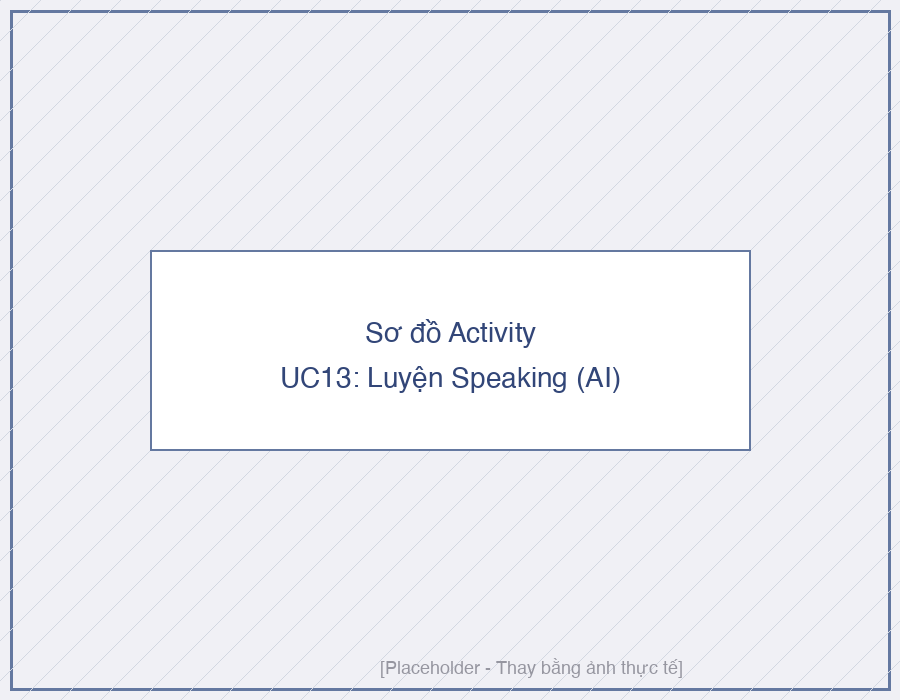
\includegraphics[width=0.85\linewidth]{activity-uc13.png}
    \caption{Sơ đồ activity UC13 -- Luyện Speaking AI Conversation}
    \label{fig:activity-uc13}
\end{figure}

\subsubsection{Mô tả kỹ thuật chi tiết}

Tính năng AI Conversation là tính năng phức tạp nhất trong hệ thống vì kết hợp ba công nghệ AI chạy nối tiếp nhau: Google Cloud Speech-to-Text (nhận dạng giọng nói), Gemini API (tạo câu hỏi và đánh giá) và Google Text-to-Speech (đọc câu hỏi cho người học nghe). Kiến trúc hệ thống sử dụng Socket.IO để duy trì kết nối WebSocket liên tục trong suốt phiên luyện tập.

Luồng xử lý cho mỗi lượt hội thoại diễn ra như sau: client gửi file audio (WAV 16kHz, mono) lên Assessment Service qua Socket.IO event \texttt{speaking:audio}. Assessment Service chuyển audio sang GCP STT API với cấu hình \texttt{languageCode: "en-US"}, \texttt{model: "latest\_long"} và \texttt{enableAutomaticPunctuation: true}. Transcript nhận được được thêm vào mảng \texttt{conversation\_history} dạng \texttt{\{role: "user", text: transcript\}}, sau đó toàn bộ mảng được gửi đến Gemini với prompt định hướng phong cách hỏi của giám khảo IELTS Speaking.

Gemini nhận diện ngữ cảnh hội thoại và trả về câu hỏi tiếp theo tự nhiên, theo đặc thù từng phần: Part 1 gồm câu hỏi đơn giản về bản thân và cuộc sống hàng ngày; Part 2 là cue card topic yêu cầu nói liên tục 2 phút; Part 3 là câu hỏi trừu tượng, thảo luận quan điểm xã hội. Câu hỏi của AI được chuyển thành audio qua Google TTS API và phát cho người học qua Socket.IO event \texttt{speaking:question}. Sau phiên luyện tập, toàn bộ \texttt{conversation\_history} được gửi đến Gemini để phân tích và đưa ra band điểm ước tính theo 4 tiêu chí IELTS Speaking chính thức.

\subsection{Thi thử IELTS -- Mock Test (UC14)}
\subsubsection{Mô tả use case}
\begin{table}[!ht]
    \centering
    \renewcommand{\arraystretch}{1.1}
    \begin{tabularx}{\linewidth}{|X|X|}
        \hline
        \multicolumn{2}{|l|}{\textbf{Đặc tả use case}} \\ \hline
        \multicolumn{2}{|l|}{\textbf{Mã use case:} UC14} \\ \hline
        \multicolumn{2}{|l|}{\textbf{Actor:} Người học} \\ \hline
        \multicolumn{2}{|p{\dimexpr\linewidth-2\tabcolsep-2\arrayrulewidth}|}{\textbf{Tiền điều kiện (Pre-condition):} Người học đã đăng nhập và chọn đề thi Mock Test (toàn phần hoặc theo từng kỹ năng).} \\ \hline
        \multicolumn{2}{|p{\dimexpr\linewidth-2\tabcolsep-2\arrayrulewidth}|}{\textbf{Hậu điều kiện (Post-condition):} Hệ thống lưu toàn bộ bài làm, quy đổi band điểm và hiển thị báo cáo kết quả đầy đủ theo từng kỹ năng.} \\ \hline
        \multicolumn{2}{|l|}{\textbf{Luồng sự kiện chính (Basic Flow)}} \\ \hline
        \textbf{Tác nhân} & \textbf{Hệ thống} \\ \hline

        1. Người học chọn đề Mock Test và xác nhận bắt đầu. & \\ \hline

        & 2. Hệ thống tạo phiên thi mới trong cơ sở dữ liệu với timestamp bắt đầu và thời gian giới hạn từng section (Listening: 30 phút; Reading: 60 phút; Writing: 60 phút; Speaking: 15 phút). \\ \hline

        & 3. Hệ thống hiển thị section Listening (4 sections, 40 câu) cùng đồng hồ đếm ngược đồng bộ server. \\ \hline

        4. Người học nghe audio và trả lời câu hỏi. Hệ thống tự động lưu câu trả lời mỗi 30 giây. & \\ \hline

        & 5. Hết giờ Listening: hệ thống tự động chuyển sang section Reading (3 passages, 40 câu) với đồng hồ mới. \\ \hline

        5. Người học hoàn thành Reading, hệ thống chuyển sang Writing rồi Speaking theo thứ tự. & \\ \hline

        6. Người học nộp bài sau khi hoàn thành Speaking hoặc hết giờ. & \\ \hline

        & 7. Hệ thống chấm tự động Listening và Reading (raw score $\rightarrow$ band theo bảng quy đổi IELTS). Writing và Speaking được gửi đến Gemini để chấm AI. \\ \hline

        & 8. Hệ thống tính Overall band bằng trung bình cộng 4 kỹ năng, làm tròn xuống bội số 0.5 gần nhất, và hiển thị báo cáo kết quả đầy đủ. \\ \hline

        \multicolumn{2}{|l|}{\textbf{Luồng sự kiện thay thế (Alternative Flow)}} \\ \hline

        & 4a. Người học thoát giữa chừng: hệ thống cảnh báo; nếu xác nhận, bài thi được lưu trạng thái "tạm dừng" và có thể tiếp tục trong 2 giờ. \\ \hline

        & (Reload trang): hệ thống tự động khôi phục phiên thi từ lần auto-save cuối nhờ \texttt{exam\_session\_id} lưu trong localStorage. \\ \hline

    \end{tabularx}
    \caption{Đặc tả Use-case Thi thử IELTS -- Mock Test (UC14)}
    \label{tab:uc14_spec}
\end{table}

\subsubsection{Sơ đồ activity}
\begin{figure}[H]
    \centering
    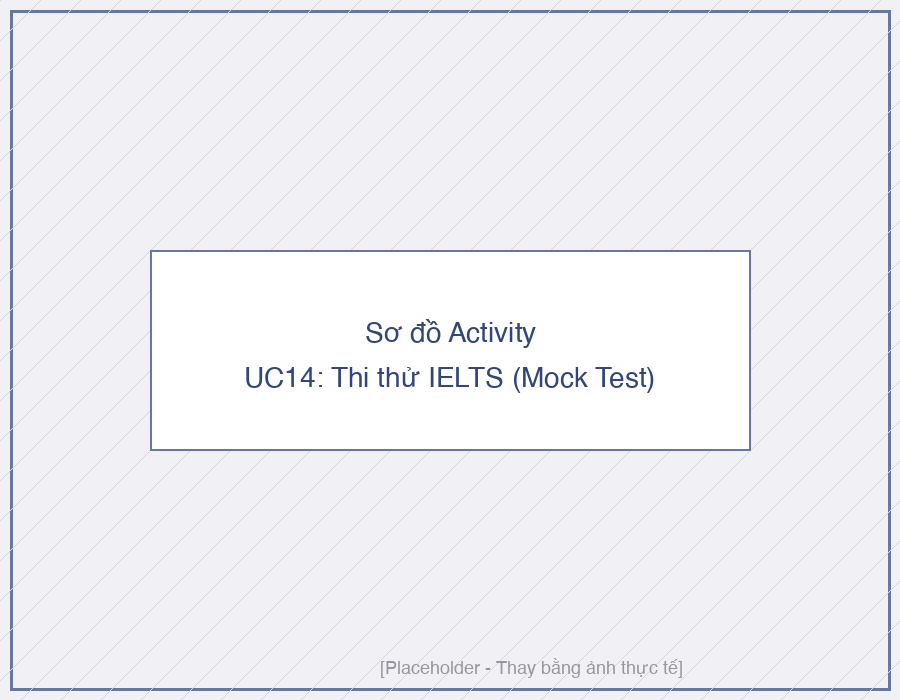
\includegraphics[width=0.85\linewidth]{activity-uc14.png}
    \caption{Sơ đồ activity UC14 -- Thi thử IELTS (Mock Test)}
    \label{fig:activity-uc14}
\end{figure}

\subsubsection{Mô tả kỹ thuật chi tiết}

Mock Test là use case đòi hỏi độ chính xác cao nhất về thời gian và tính toàn vẹn dữ liệu. Cơ chế đồng hồ đếm ngược được thiết kế phía server để tránh gian lận: khi bắt đầu mỗi section, Exam Service ghi \texttt{section\_start\_at} và \texttt{section\_deadline = now() + duration} vào bảng \texttt{exam\_sessions}. Client nhận \texttt{section\_deadline} qua Socket.IO và tính thời gian còn lại bằng \texttt{deadline - Date.now()} thay vì bộ đếm local -- điều này đảm bảo đồng hồ không bị ảnh hưởng khi người dùng tải lại trang.

Cơ chế auto-save hoạt động bằng cách gọi \texttt{PATCH /exam-sessions/:id/draft} mỗi 30 giây với payload là toàn bộ câu trả lời hiện tại. Khi người học reload trang, client gửi \texttt{exam\_session\_id} (lưu trong localStorage) đến \texttt{GET /exam-sessions/:id/resume} để nhận lại trạng thái bài thi gần nhất: câu đang làm, thời gian đã trôi qua và câu trả lời đã lưu.

Hệ thống quy đổi điểm sử dụng hai bảng tra cứu riêng biệt cho Listening và Reading, phản ánh thang điểm IELTS chính thức. Ví dụ với Listening: raw score 39--40 tương ứng band 9.0; 37--38 tương ứng band 8.5; 35--36 tương ứng band 8.0. Overall band được tính theo công thức $\text{Overall} = \lfloor \frac{L + R + W + S}{4} \times 2 \rfloor \div 2$ -- nhân đôi, làm tròn xuống số nguyên, chia đôi để đạt kết quả là bội số của 0.5. Toàn bộ kết quả được lưu vào bảng \texttt{mock\_test\_results} và hiển thị trong trang báo cáo chi tiết kèm phân tích điểm mạnh/yếu từng kỹ năng.

\chapter{THIẾT KẾ VÀ HIỆN THỰC}

Chương này trình bày quá trình thiết kế và hiện thực hệ thống, bao gồm: sơ đồ lớp, sơ đồ cơ sở dữ liệu, kiến trúc phần mềm, luồng màn hình, giao diện người dùng và kết quả kiểm thử. Các sơ đồ và thiết kế được xây dựng trực tiếp từ kết quả phân tích ở Chương 3, phản ánh cách hệ thống được hiện thực bằng NestJS~\cite{nestjs-docs}, Next.js~\cite{nextjs-docs} và React Native~\cite{reactnative-docs}.

\section{Sơ đồ lớp}

Sơ đồ lớp của hệ thống IELTS Learning System được chia thành hai nhóm module nhằm tăng tính rõ ràng và dễ bảo trì: nhóm \textbf{User \& Auth} quản lý tài khoản, xác thực và hồ sơ người học; nhóm \textbf{Learning} quản lý bài tập 4 kỹ năng, từ vựng, đề thi và tiến độ học tập~\cite{fowler2002patterns}.

Trong nhóm User \& Auth, lớp \texttt{User} giữ vai trò trung tâm với các thuộc tính: \texttt{id}, \texttt{email}, \texttt{passwordHash}, \texttt{role} (learner/admin), \texttt{failedAttempts}, \texttt{lockUntil} và \texttt{createdAt}. Lớp \texttt{OtpToken} liên kết 1-nhiều với \texttt{User} thông qua \texttt{userId}, lưu mã OTP 6 chữ số và thời gian hết hạn. Lớp \texttt{RefreshToken} lưu refresh token theo từng phiên đăng nhập, cho phép vô hiệu hoá đơn lẻ khi người dùng đăng xuất trên một thiết bị cụ thể mà không ảnh hưởng các phiên khác.

Trong nhóm Learning, lớp \texttt{Skill} phân loại 4 kỹ năng (Listening, Reading, Writing, Speaking). Lớp \texttt{Exercise} liên kết với \texttt{Skill} và chứa nội dung bài tập (audio URL, passage, writing prompt). Lớp \texttt{UserExerciseResult} ghi nhận kết quả mỗi lần làm bài của từng người học theo thời gian. Lớp \texttt{VocabularyItem} và \texttt{UserVocabularyCard} hiện thực thuật toán Spaced Repetition với các trường \texttt{easeFactor} và \texttt{nextReview}. Lớp \texttt{ExamSession} và \texttt{ExamSectionDraft} quản lý phiên thi Mock Test với cơ chế auto-save và khôi phục.

\begin{figure}[H]
    \centering
    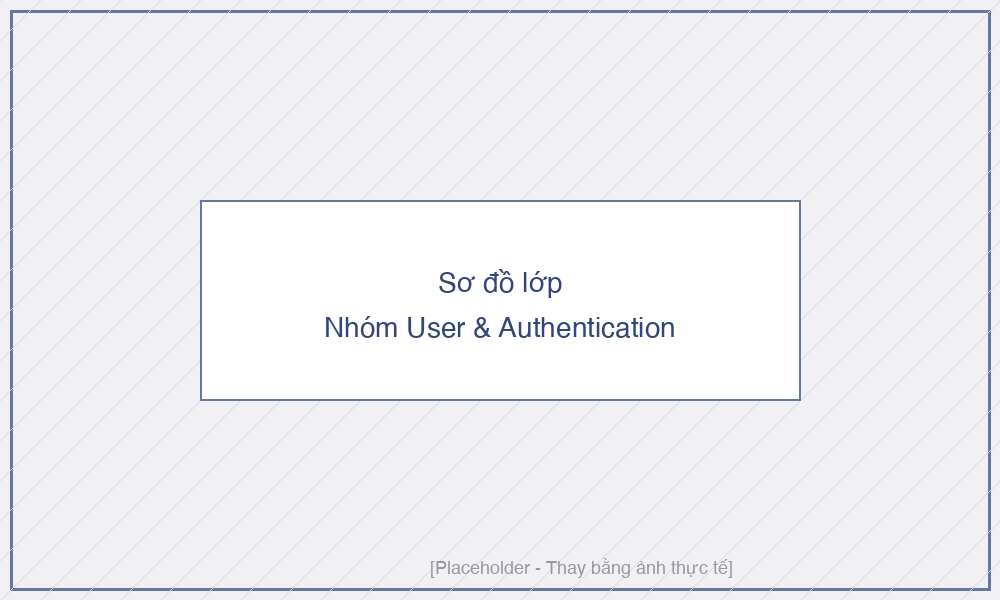
\includegraphics[width=0.95\linewidth]{class-diagram-user.png}
    \caption{Sơ đồ lớp nhóm User \& Auth}
    \label{fig:class-user}
\end{figure}

\begin{figure}[H]
    \centering
    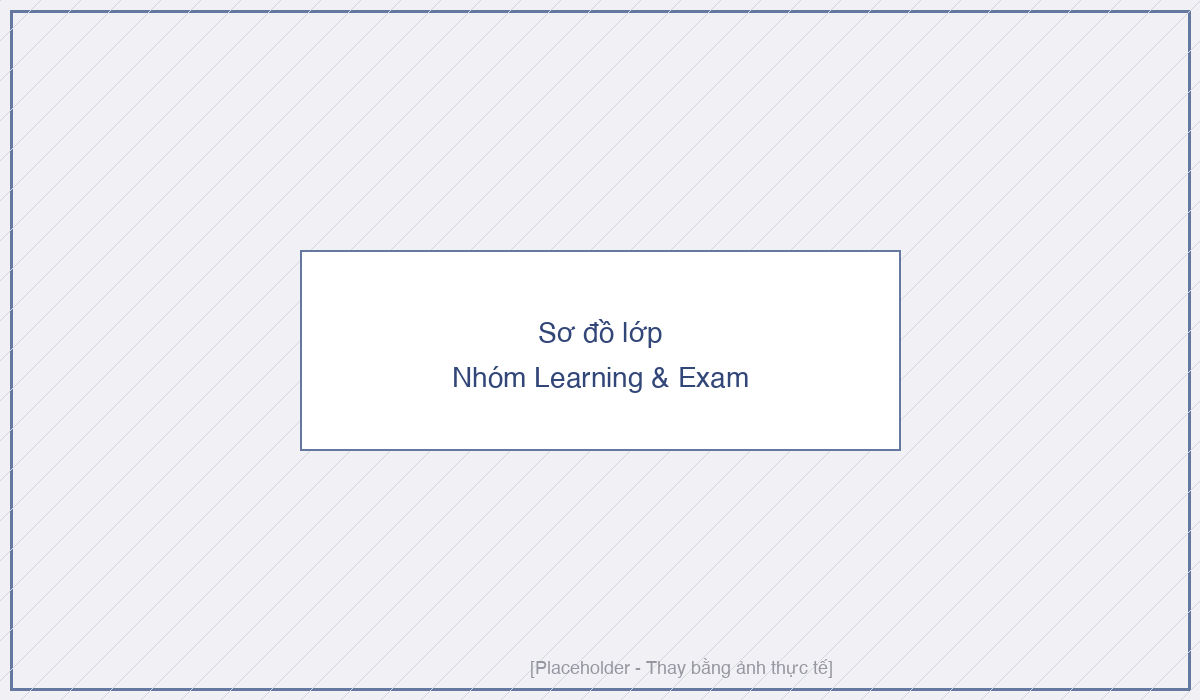
\includegraphics[width=0.95\linewidth]{class-diagram-learning.png}
    \caption{Sơ đồ lớp nhóm Learning}
    \label{fig:class-learning}
\end{figure}

\section{Sơ đồ cơ sở dữ liệu}

\subsection{Sơ đồ cơ sở dữ liệu có cấu trúc (SQL)}

Hệ thống sử dụng PostgreSQL~\cite{postgresql-docs} được quản lý thông qua Supabase~\cite{supabase-docs} và Prisma ORM~\cite{prisma-docs}. Toàn bộ schema được định nghĩa trong file \texttt{schema.prisma} và ánh xạ sang các bảng quan hệ trong PostgreSQL thông qua Prisma Migrate. Sơ đồ ERD (Entity-Relationship Diagram) bên dưới thể hiện các bảng chính cùng quan hệ giữa chúng.

Các bảng cốt lõi được tổ chức theo nhóm: nhóm xác thực gồm \texttt{users}, \texttt{otp\_tokens}, \texttt{refresh\_tokens}; nhóm bài tập gồm \texttt{skills}, \texttt{exercises}, \texttt{exercise\_options}, \texttt{user\_exercise\_results}; nhóm từ vựng gồm \texttt{vocabulary\_items}, \texttt{user\_vocabulary\_cards}; nhóm thi thử gồm \texttt{exam\_papers}, \texttt{exam\_sessions}, \texttt{exam\_section\_drafts}, \texttt{mock\_test\_results}. Khóa ngoại được thiết lập đầy đủ với \texttt{ON DELETE CASCADE} ở các bảng con để đảm bảo tính toàn vẹn dữ liệu khi xoá bản ghi cha.

\begin{figure}[H]
    \centering
    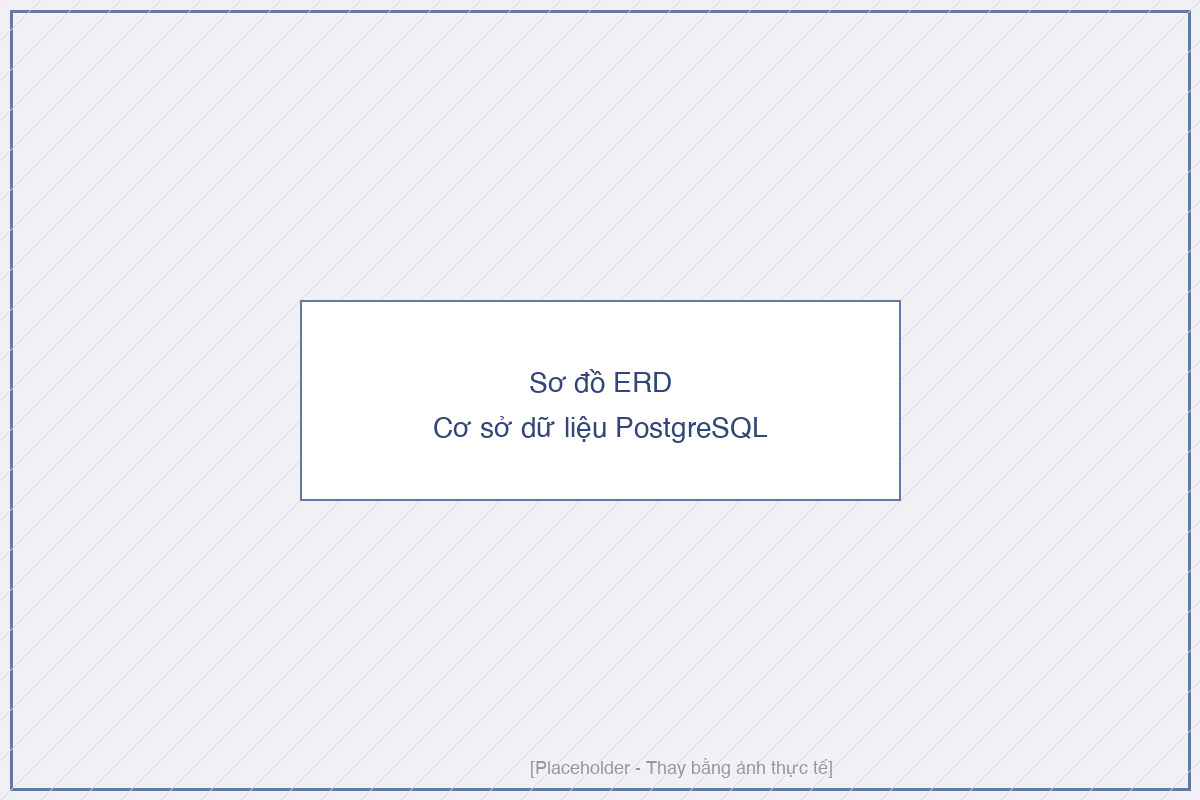
\includegraphics[width=\linewidth]{erd-sql.png}
    \caption{Sơ đồ cơ sở dữ liệu quan hệ (ERD -- PostgreSQL)}
    \label{fig:erd-sql}
\end{figure}

\section{Sơ đồ kiến trúc phần mềm}

Hệ thống IELTS Learning System được xây dựng theo kiến trúc Microservices~\cite{newman2015microservices}, trong đó mỗi service chịu trách nhiệm một nghiệp vụ độc lập và giao tiếp qua REST API nội bộ hoặc Socket.IO. Toàn bộ yêu cầu từ client đều đi qua một \textbf{API Gateway} (NestJS) trước khi được định tuyến đến service phù hợp.

Các microservice chính bao gồm: \textbf{User Service} xử lý đăng ký, đăng nhập, quản lý hồ sơ và xác thực JWT; \textbf{Content Service} quản lý bài tập, đề thi và từ vựng; \textbf{Assessment Service} gọi Gemini API để chấm Writing/Speaking và GCP STT để chuyển đổi giọng nói; \textbf{Exam Service} quản lý phiên thi Mock Test, đồng hồ server và cơ chế auto-save. Tầng dữ liệu sử dụng PostgreSQL qua Supabase, đồng thời Supabase Storage lưu trữ file audio và hình ảnh bài tập. Client gồm Next.js (Web) và React Native (Mobile) kết nối với API Gateway qua HTTPS và WebSocket (Socket.IO)~\cite{socketio-docs}.

\begin{figure}[H]
    \centering
    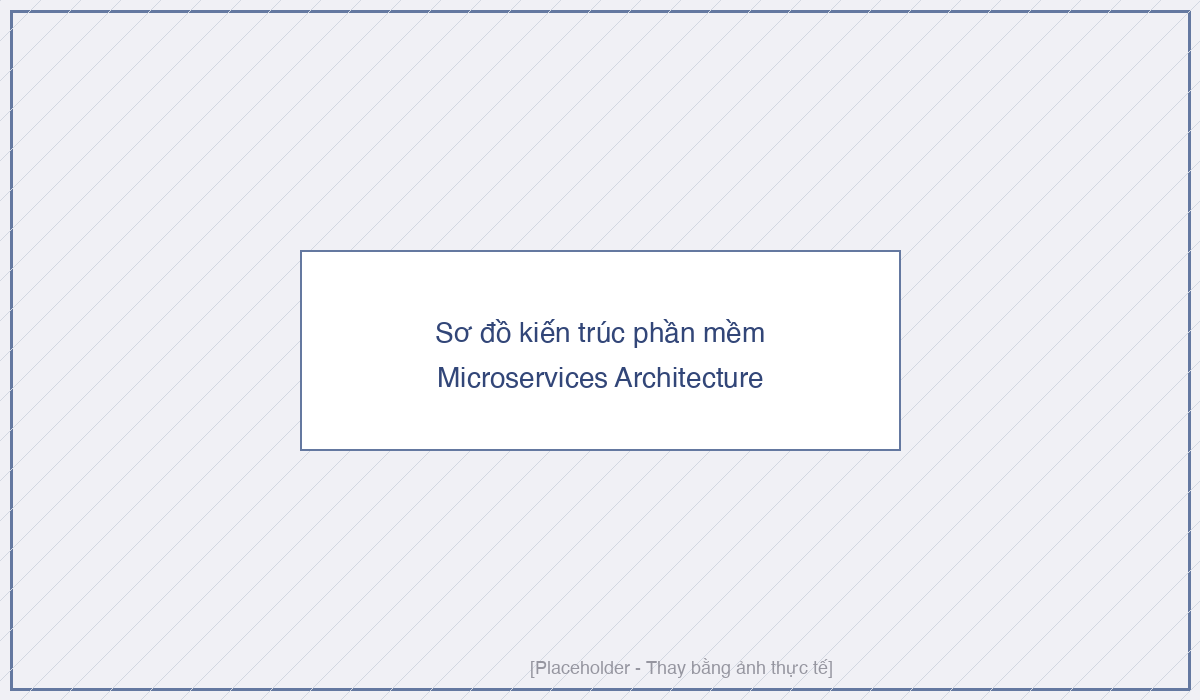
\includegraphics[width=\linewidth]{architecture.png}
    \caption{Sơ đồ kiến trúc phần mềm hệ thống IELTS Learning System}
    \label{fig:architecture}
\end{figure}

\section{Sơ đồ luồng màn hình}

\subsection{Sơ đồ luồng màn hình website}

Trên nền tảng Web (Next.js), người dùng bắt đầu từ \textbf{Landing Page}, tiếp tục đến màn hình \textbf{Đăng nhập / Đăng ký}, sau đó vào \textbf{Dashboard} chính. Từ Dashboard, người học có thể chuyển sang 4 nhánh chính: \textbf{Luyện kỹ năng} (Listening / Reading / Writing / Speaking), \textbf{Từ vựng} (học mới và ôn luyện flashcard), \textbf{Mock Test} (chọn đề và làm bài toàn phần), và \textbf{Kết quả} (xem báo cáo tiến độ). Người quản lý (Admin) có nhánh riêng dẫn vào \textbf{Admin Dashboard} với các chức năng quản lý nội dung, đề thi và học viên.

\begin{figure}[H]
    \centering
    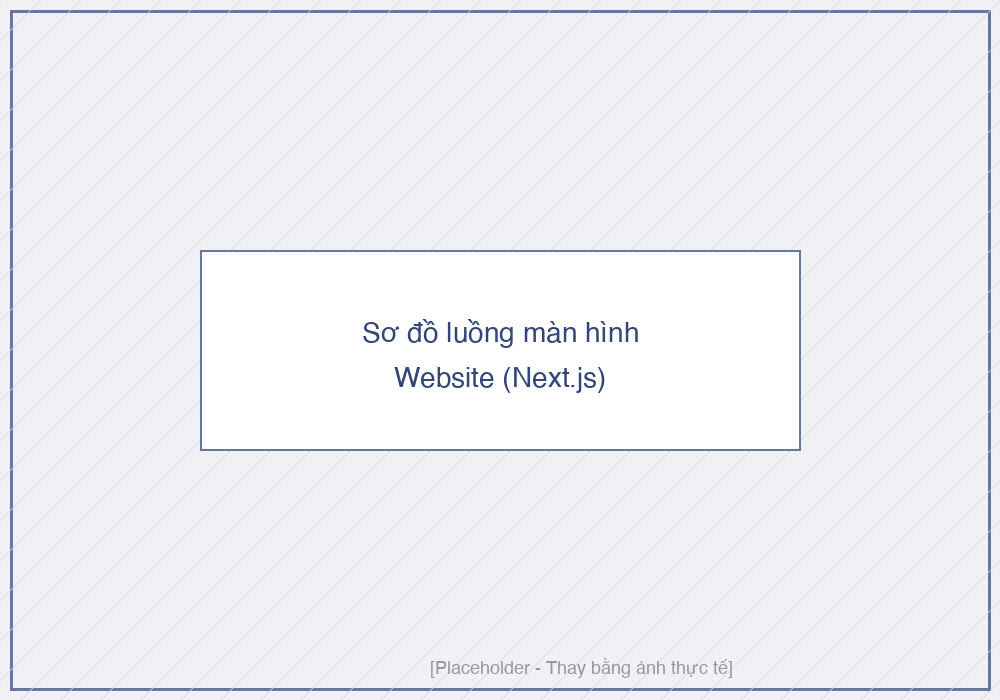
\includegraphics[width=\linewidth]{flow-web.png}
    \caption{Sơ đồ luồng màn hình website (Next.js)}
    \label{fig:flow-web}
\end{figure}

\subsection{Sơ đồ luồng màn hình mobile}

Trên nền tảng Mobile (React Native), cấu trúc điều hướng sử dụng Tab Navigation ở tầng dưới cùng với 4 tab chính: \textbf{Trang chủ}, \textbf{Luyện tập}, \textbf{Từ vựng} và \textbf{Hồ sơ}. Các màn hình con được quản lý bằng Stack Navigator. Luồng Mock Test trên mobile được thiết kế dạng fullscreen để tránh xao nhãng, với thanh điều hướng section cố định phía trên và nút đếm câu đã trả lời phía dưới.

\begin{figure}[H]
    \centering
    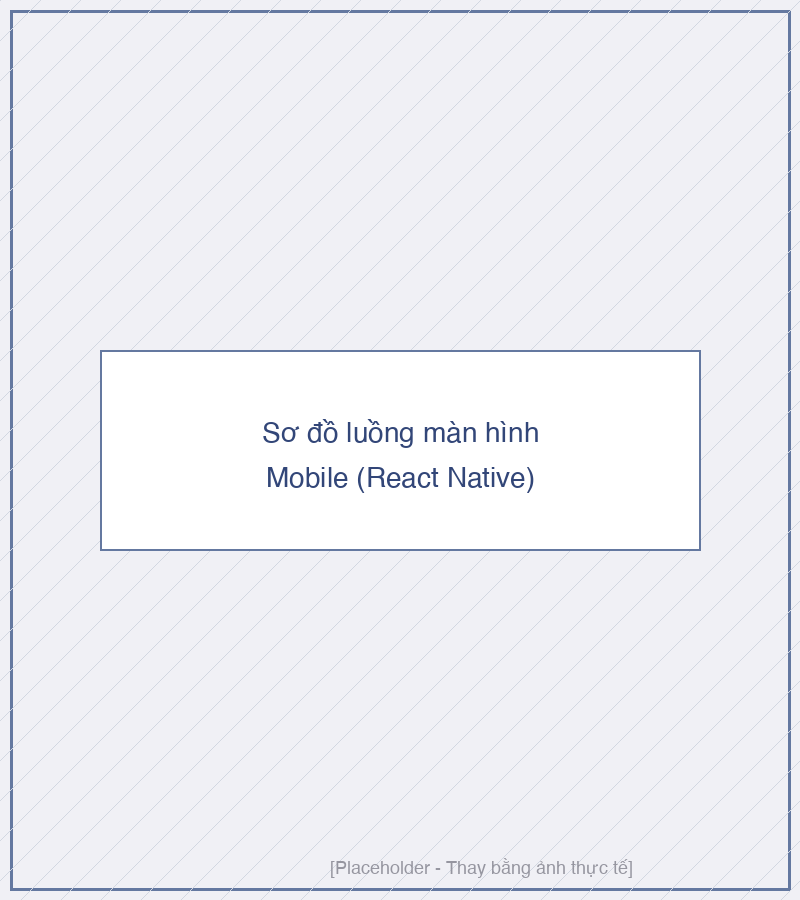
\includegraphics[width=0.7\linewidth]{flow-mobile.png}
    \caption{Sơ đồ luồng màn hình mobile (React Native)}
    \label{fig:flow-mobile}
\end{figure}

\section{Giao diện chương trình}

Phần này trình bày các giao diện chính của hệ thống trên cả hai nền tảng Web và Mobile, thể hiện kết quả hiện thực thực tế của các use case đã phân tích ở Chương 3.

\subsection{Giao diện trang chủ (Landing Page)}

Trang chủ giới thiệu tổng quan hệ thống với banner nêu bật tính năng AI scoring, thanh điều hướng nhanh đến 4 kỹ năng và nút kêu gọi hành động (CTA) dẫn đến trang đăng ký. Giao diện sử dụng TailwindCSS với bảng màu xanh dương -- trắng nhất quán, đảm bảo tính chuyên nghiệp và dễ đọc.

\begin{figure}[H]
    \centering
    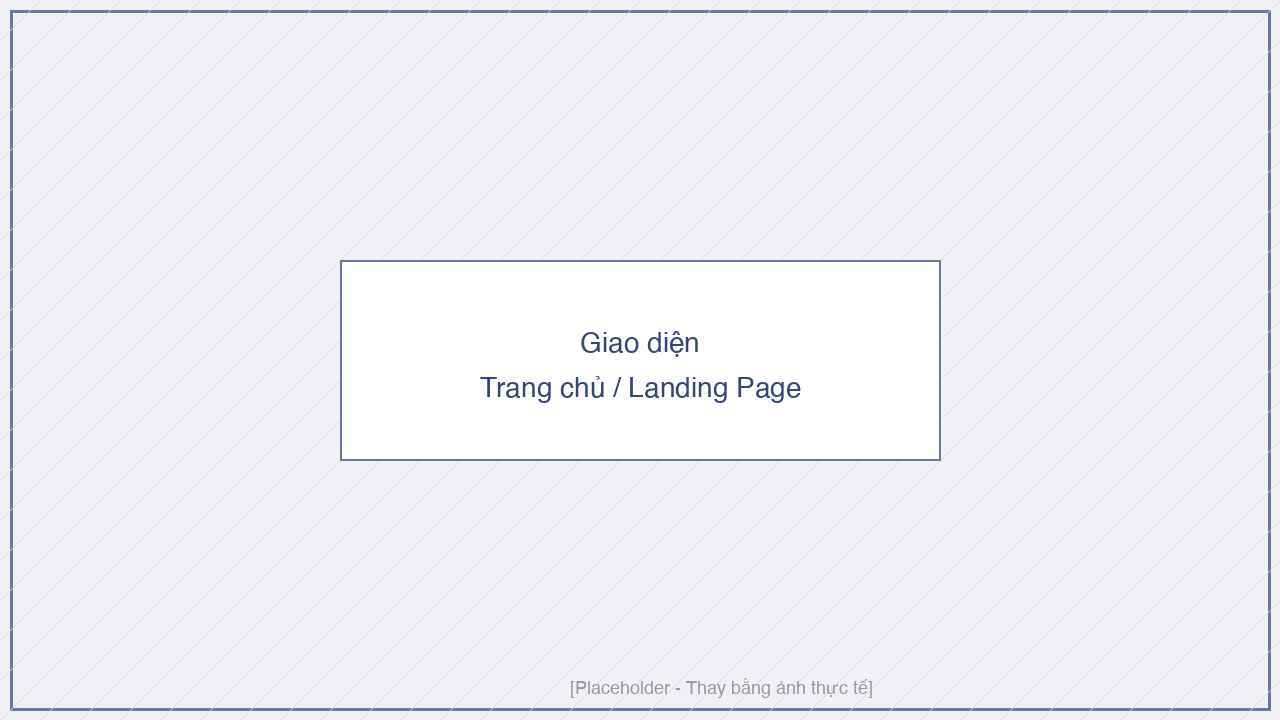
\includegraphics[width=\linewidth]{ui-landing.png}
    \caption{Giao diện trang chủ (Landing Page)}
    \label{fig:ui-landing}
\end{figure}

\subsection{Giao diện Dashboard người học}

Dashboard hiển thị tóm tắt tiến độ học tập theo tuần, bao gồm: biểu đồ điểm từng kỹ năng, chuỗi ngày học liên tiếp (streak), số từ vựng cần ôn hôm nay theo Spaced Repetition và danh sách bài luyện gần đây. Bố cục dạng lưới 2 cột: cột trái là biểu đồ thống kê, cột phải là lịch học và thông báo từ hệ thống.

\begin{figure}[H]
    \centering
    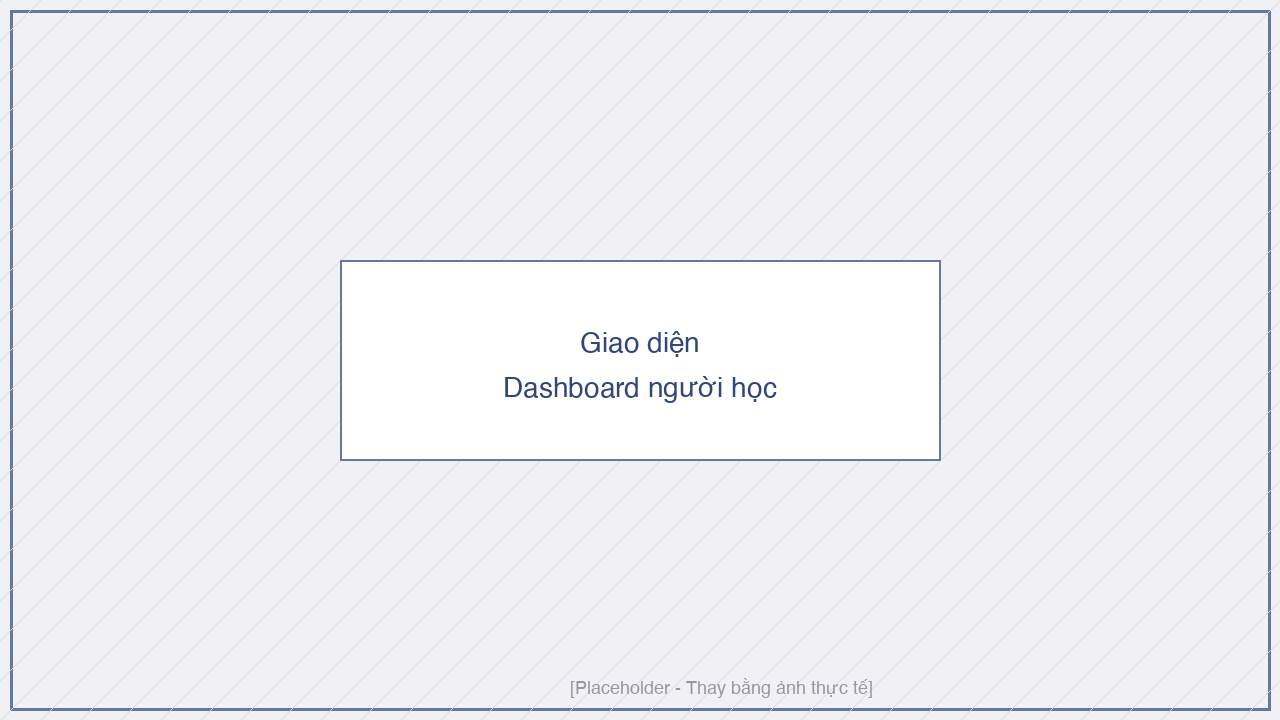
\includegraphics[width=\linewidth]{ui-dashboard.png}
    \caption{Giao diện Dashboard người học}
    \label{fig:ui-dashboard}
\end{figure}

\subsection{Giao diện Luyện Listening}

Giao diện Listening gồm audio player tùy chỉnh (hỗ trợ điều chỉnh tốc độ 0.75x -- 1.5x và cuộn lại 10 giây), phía dưới là khu vực câu hỏi đa dạng (Multiple Choice, Short Answer, Matching, Labelling). Sau khi nộp bài, giao diện chuyển sang trang kết quả: câu đúng hiển thị màu xanh lá, câu sai màu đỏ kèm đáp án đúng và phân tích loại lỗi (Wrong Word / Missing Word / Extra Word) cho dạng Short Answer.

\begin{figure}[H]
    \centering
    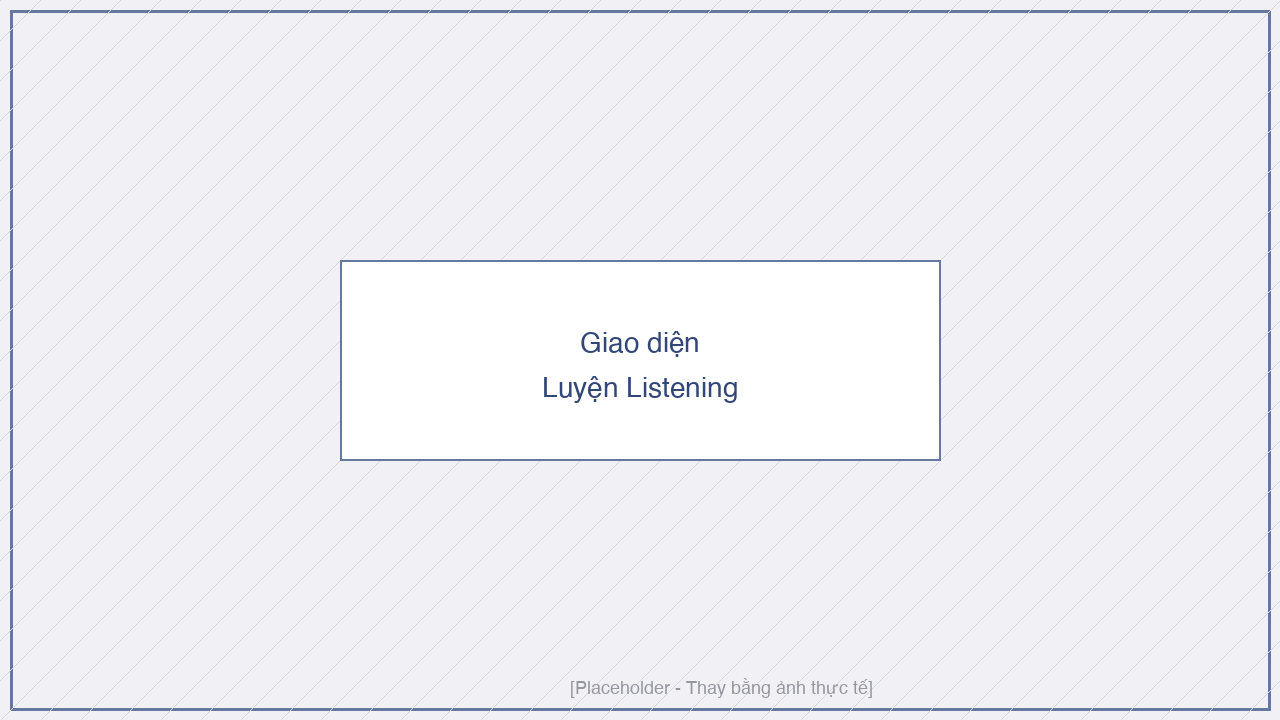
\includegraphics[width=\linewidth]{ui-listening.png}
    \caption{Giao diện luyện Listening}
    \label{fig:ui-listening}
\end{figure}

\subsection{Giao diện Luyện Reading}

Giao diện Reading sử dụng layout 2 cột: cột trái (60\% chiều rộng) hiển thị đoạn văn với hỗ trợ highlight từ khoá khi di chuột; cột phải (40\%) hiển thị các câu hỏi. Hai cột có thanh cuộn độc lập, giúp người học vừa đọc vừa trả lời mà không cần cuộn trang nhiều lần -- đây là điểm cải tiến đáng kể so với giao diện luyện Reading thông thường.

\begin{figure}[H]
    \centering
    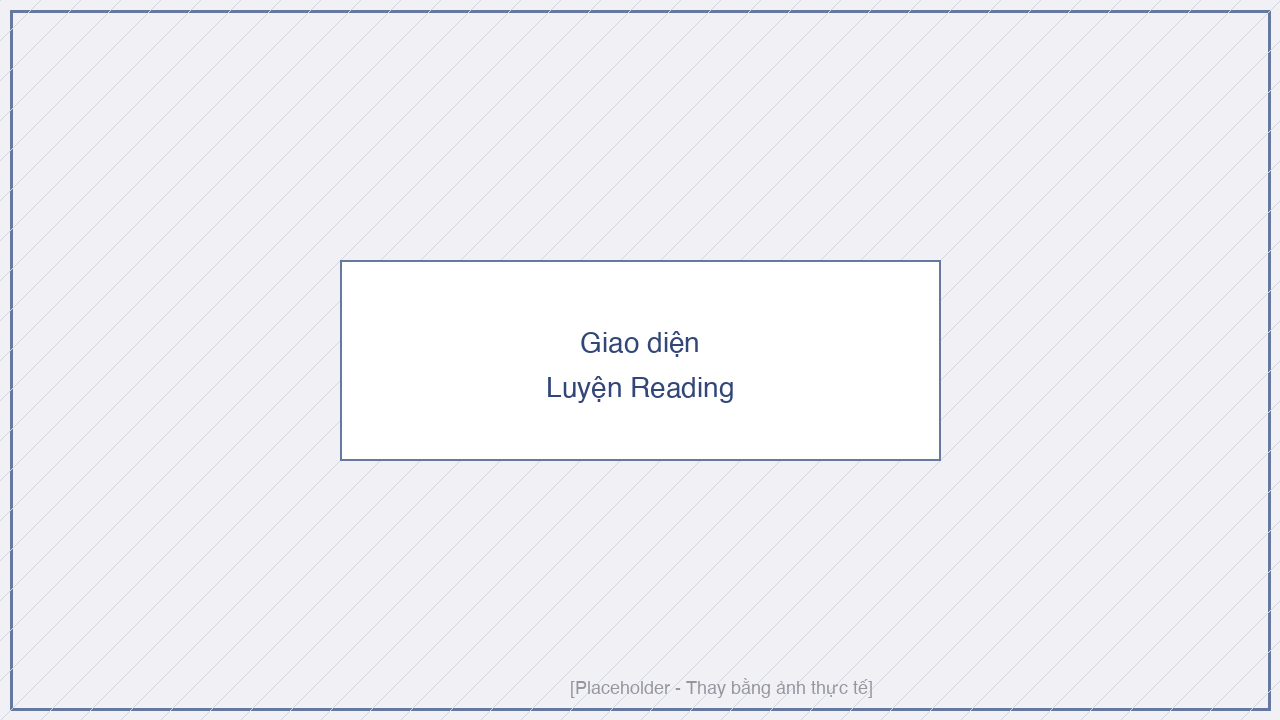
\includegraphics[width=\linewidth]{ui-reading.png}
    \caption{Giao diện luyện Reading}
    \label{fig:ui-reading}
\end{figure}

\subsection{Giao diện Luyện Writing và phản hồi AI}

Giao diện Writing gồm 2 tab: tab \textbf{Đề bài} hiển thị topic, task type và yêu cầu số từ; tab \textbf{Bài làm} là textarea với bộ đếm từ real-time ở góc phải. Sau khi nộp bài, màn hình phản hồi AI hiển thị điểm từng tiêu chí (TA, CC, LR, GRA), Overall band nổi bật ở đầu trang và nhận xét chi tiết dạng văn xuôi với các điểm mạnh được highlight xanh và điểm cần cải thiện highlight vàng.

\begin{figure}[H]
    \centering
    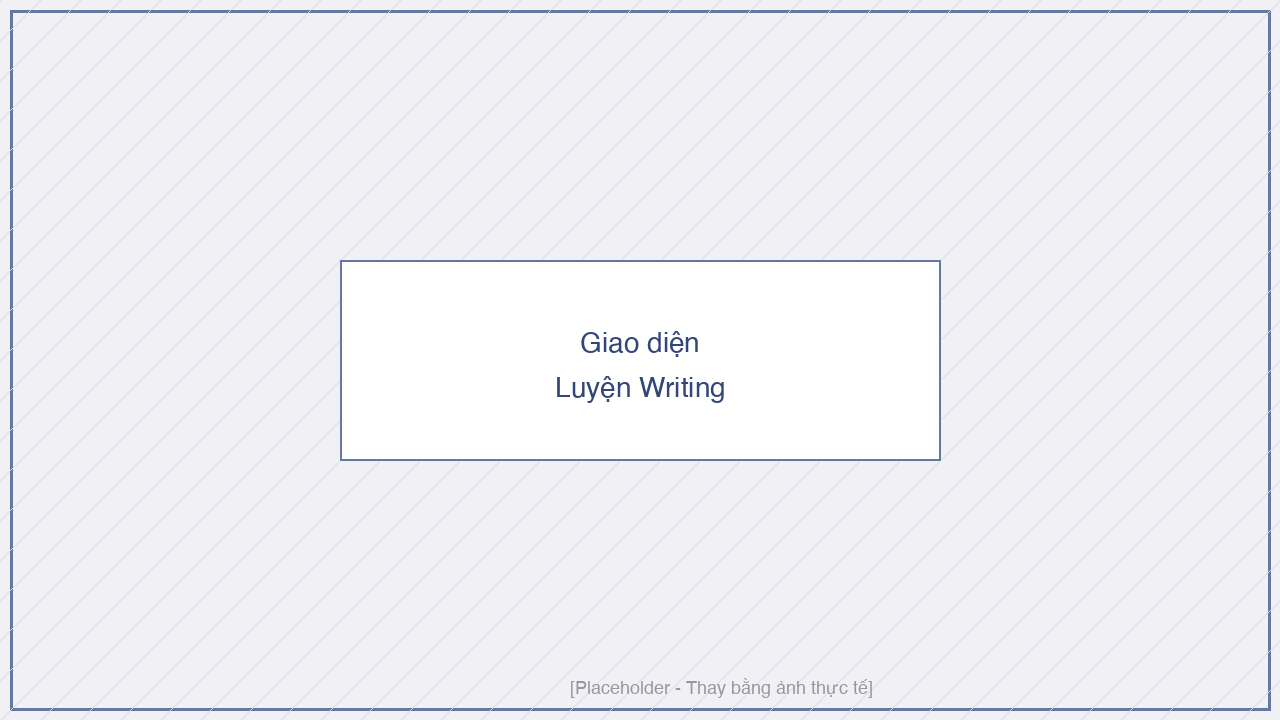
\includegraphics[width=\linewidth]{ui-writing.png}
    \caption{Giao diện luyện Writing -- Đề bài và khu vực soạn thảo}
    \label{fig:ui-writing}
\end{figure}

\begin{figure}[H]
    \centering
    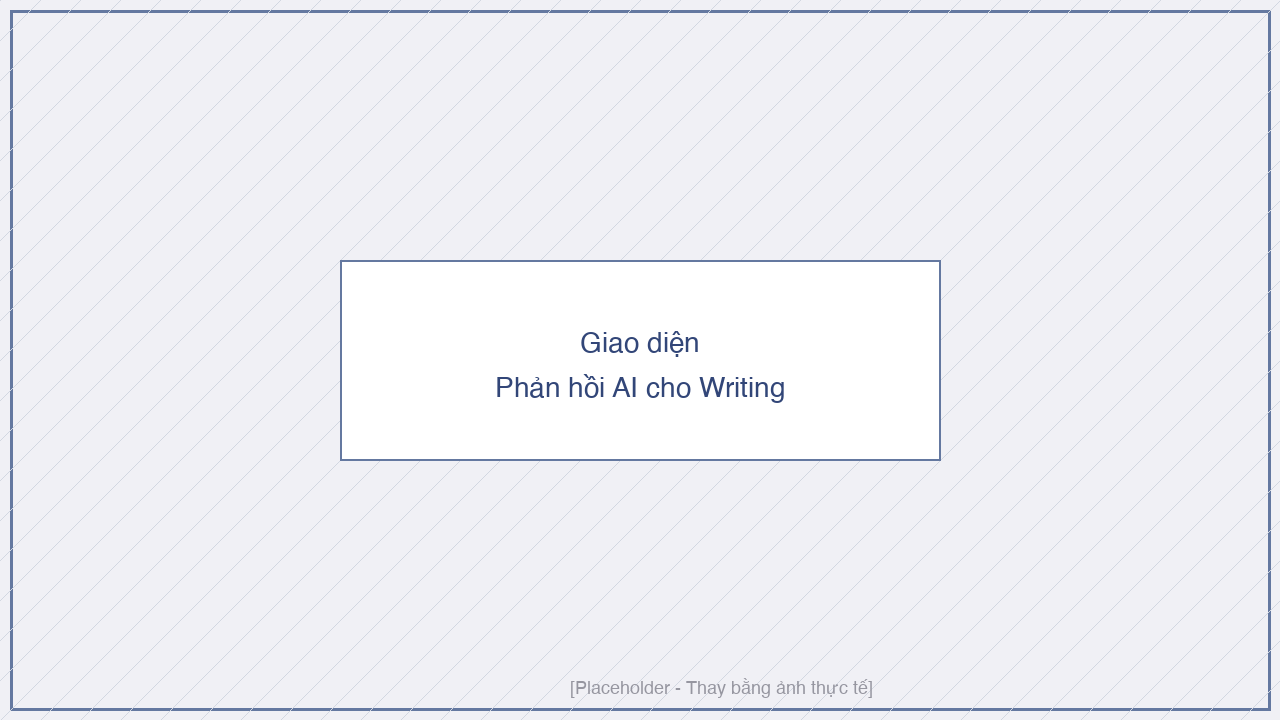
\includegraphics[width=\linewidth]{ui-writing-feedback.png}
    \caption{Giao diện phản hồi AI cho bài Writing}
    \label{fig:ui-writing-feedback}
\end{figure}

\subsection{Giao diện Luyện Speaking}

Giao diện Speaking hiển thị chủ đề hội thoại và câu hỏi hiện tại của AI. Người học nhấn giữ nút microphone để ghi âm; thanh sóng âm (waveform) hiển thị trực quan xác nhận đang thu âm thành công. Sau mỗi lượt, transcript của người học xuất hiện và câu hỏi tiếp theo của AI được phát qua loa tự động. Cuối phiên, trang kết quả hiển thị band ước tính theo 4 tiêu chí và transcript toàn bộ cuộc hội thoại để người học tự phân tích.

\begin{figure}[H]
    \centering
    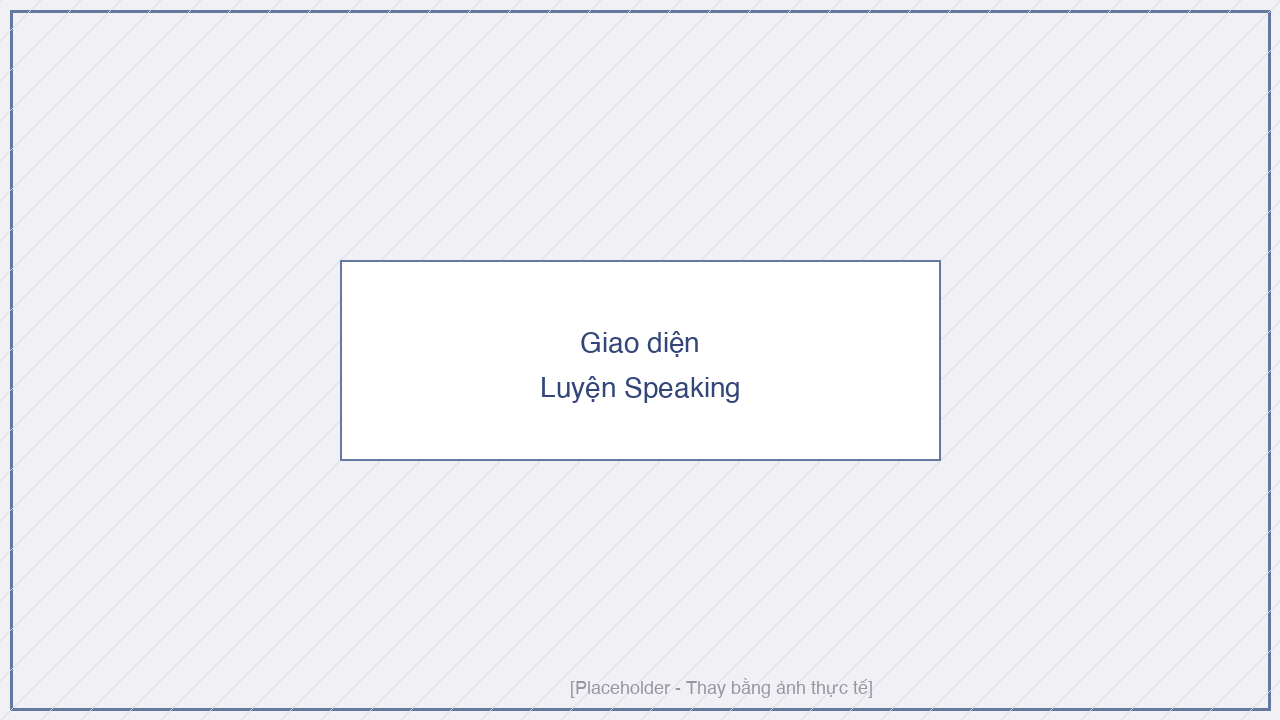
\includegraphics[width=\linewidth]{ui-speaking.png}
    \caption{Giao diện luyện Speaking -- AI Conversation}
    \label{fig:ui-speaking}
\end{figure}

\subsection{Giao diện Mock Test}

Giao diện Mock Test hiển thị toàn màn hình với: tiêu đề section hiện tại (Listening / Reading / Writing / Speaking), đồng hồ đếm ngược ở góc trên phải (chuyển màu đỏ khi còn dưới 5 phút), và thanh điều hướng câu hỏi dạng lưới số ở cột bên phải (xanh lá = đã trả lời, trắng = chưa trả lời). Khi hết giờ mỗi section, hệ thống tự động submit và chuyển sang section tiếp theo mà không yêu cầu thao tác từ người học.

\begin{figure}[H]
    \centering
    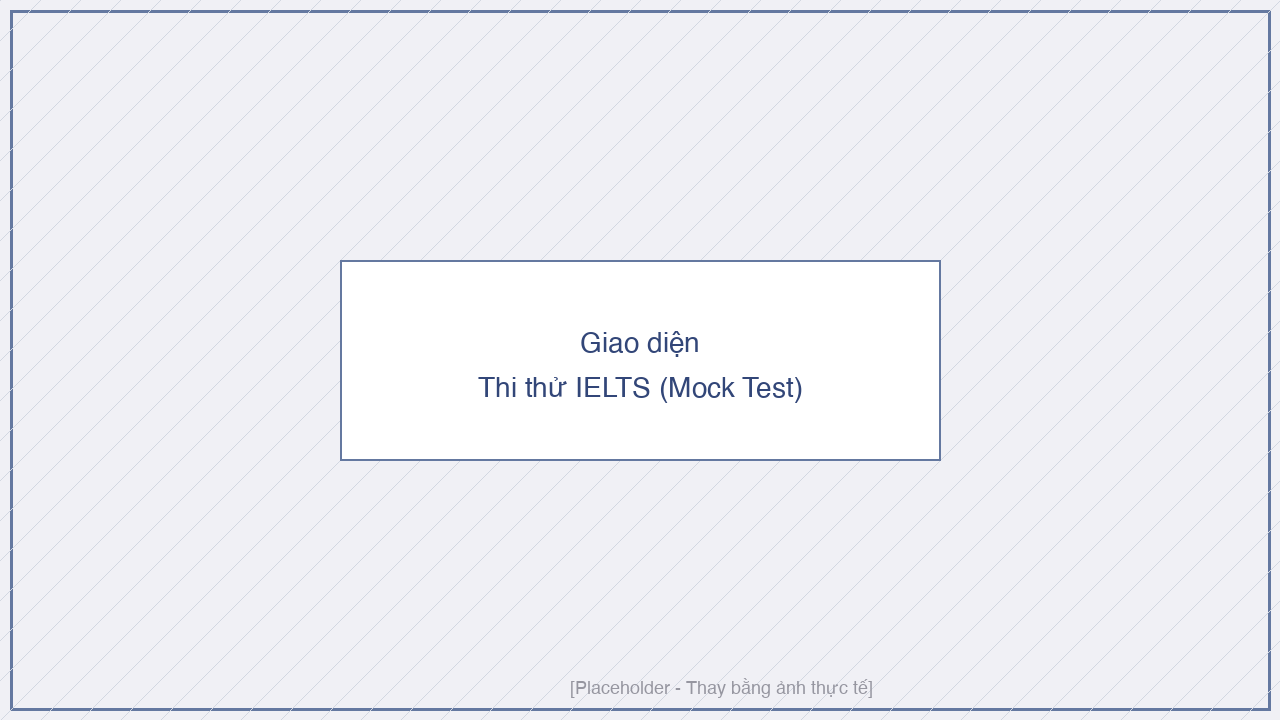
\includegraphics[width=\linewidth]{ui-mocktest.png}
    \caption{Giao diện Mock Test -- Giao diện làm bài}
    \label{fig:ui-mocktest}
\end{figure}

\subsection{Giao diện kết quả và tiến độ}

Trang kết quả Mock Test hiển thị Overall band nổi bật ở trung tâm, tiếp theo là biểu đồ radar (spider chart) thể hiện 4 kỹ năng và bên dưới là phân tích chi tiết từng kỹ năng (số câu đúng/sai với Listening/Reading; nhận xét AI với Writing/Speaking). Trang tiến độ học tập dài hạn hiển thị biểu đồ cột theo tuần và lịch học dạng heatmap tương tự GitHub contribution graph.

\begin{figure}[H]
    \centering
    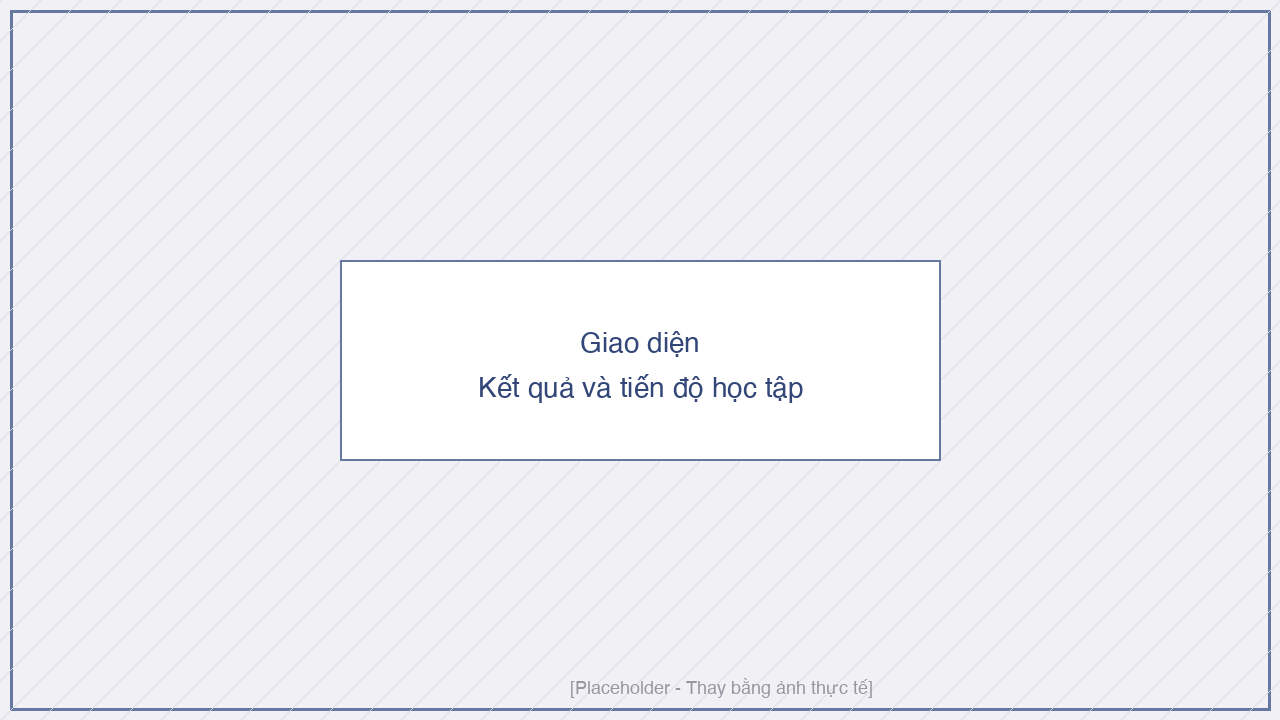
\includegraphics[width=\linewidth]{ui-result.png}
    \caption{Giao diện kết quả Mock Test và báo cáo tiến độ}
    \label{fig:ui-result}
\end{figure}

\subsection{Giao diện Từ vựng và Flashcard}

Giao diện từ vựng gồm hai chế độ: chế độ \textbf{Học mới} dùng flashcard lật với nút nhớ / quên để cập nhật ease factor; chế độ \textbf{Ôn luyện} dùng quiz trắc nghiệm 4 đáp án. Danh sách từ vựng hiển thị dạng bảng với các cột: từ, phiên âm, nghĩa, ngày ôn tiếp theo và trạng thái (New / Learning / Review / Mature). Trên Mobile, flashcard hỗ trợ gesture vuốt phải (nhớ) và vuốt trái (quên) để thao tác nhanh hơn.

\begin{figure}[H]
    \centering
    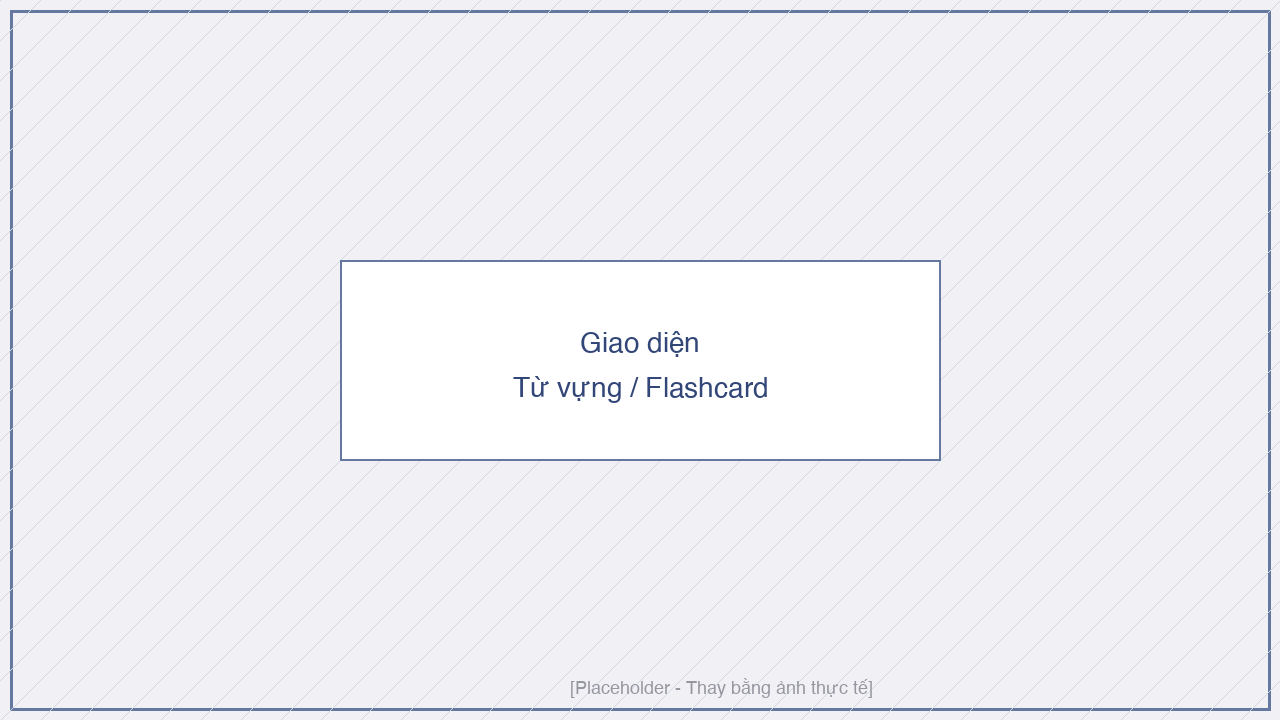
\includegraphics[width=\linewidth]{ui-vocabulary.png}
    \caption{Giao diện từ vựng và flashcard (Spaced Repetition)}
    \label{fig:ui-vocabulary}
\end{figure}

\subsection{Giao diện Admin}

Giao diện Admin sử dụng sidebar navigation với các mục: \textbf{Tổng quan} (thống kê số người dùng, lượt làm bài theo ngày, phân phối band điểm); \textbf{Quản lý nội dung} (thêm/sửa/xóa bài tập theo từng kỹ năng, bao gồm upload audio cho Listening); \textbf{Quản lý đề thi} (tạo và phân bổ đề Mock Test, thiết lập thời gian từng section); \textbf{Quản lý học viên} (xem danh sách người dùng, xem tiến độ từng học viên, khoá tài khoản); \textbf{Thống kê} (báo cáo biểu đồ tăng trưởng người dùng và điểm trung bình theo thời gian).

\begin{figure}[H]
    \centering
    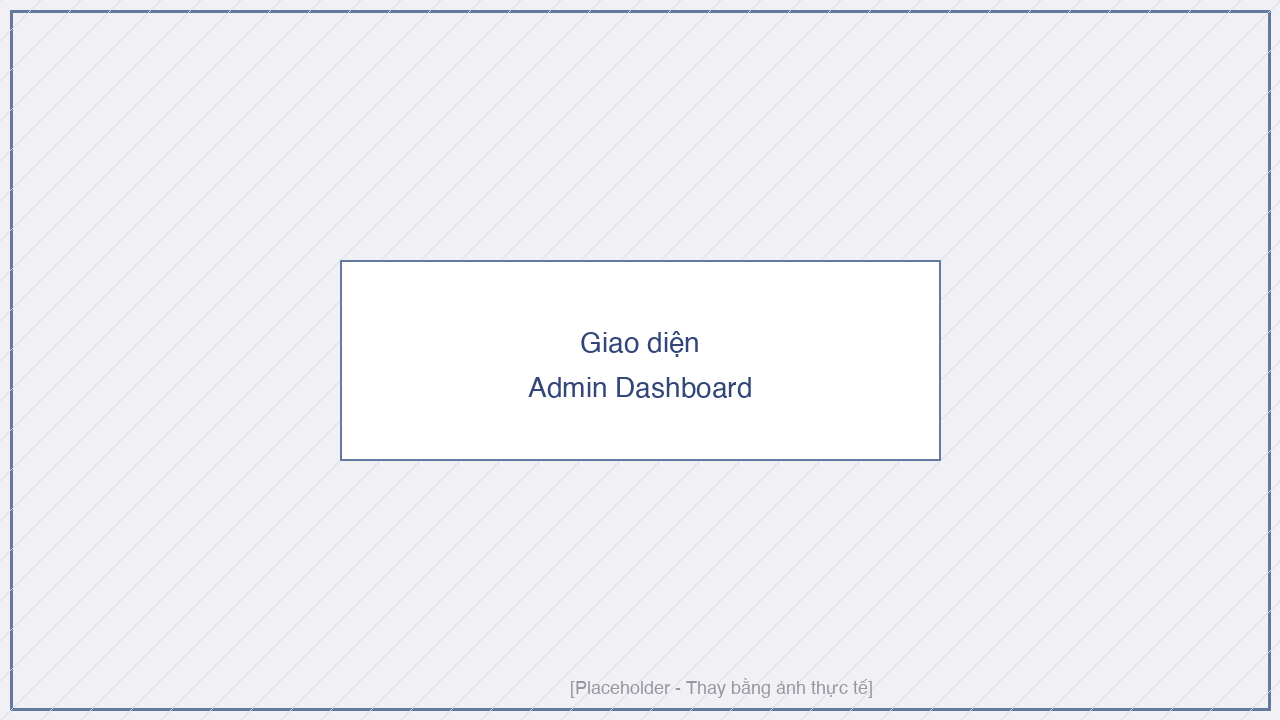
\includegraphics[width=\linewidth]{ui-admin.png}
    \caption{Giao diện Admin -- Trang tổng quan và quản lý}
    \label{fig:ui-admin}
\end{figure}

\section{Kiểm thử hệ thống}

\subsection{Danh sách các test case}

Chúng em thực hiện kiểm thử hộp đen (Black-box Testing) cho các chức năng chính của hệ thống. Mỗi test case bao gồm mã định danh, chức năng kiểm tra, tiền điều kiện, tình huống thực hiện và kết quả mong đợi. Tổng cộng 22 tình huống kiểm thử được xây dựng cho 7 nhóm chức năng cốt lõi.

\renewcommand{\arraystretch}{1.2}
\begin{longtable}{|p{1.3cm}|p{2.8cm}|p{2.8cm}|p{4.0cm}|p{3.0cm}|}
    \caption{Danh sách các test case}
    \label{tab:testcase_list} \\
    \hline
    \textbf{Mã TC} & \textbf{Chức năng} & \textbf{Tiền điều kiện} & \textbf{Tình huống} & \textbf{Kết quả mong đợi} \\ \hline
    \endfirsthead
    \multicolumn{5}{r}{\textit{(tiếp trang trước)}} \\
    \hline
    \textbf{Mã TC} & \textbf{Chức năng} & \textbf{Tiền điều kiện} & \textbf{Tình huống} & \textbf{Kết quả mong đợi} \\ \hline
    \endhead
    \hline \multicolumn{5}{r}{\textit{(tiếp trang sau)}} \\
    \endfoot
    \hline
    \endlastfoot

    TC01-01 & Đăng ký tài khoản & Email chưa tồn tại trong hệ thống & Nhập email hợp lệ, mật khẩu $\geq$8 ký tự & Gửi OTP về email, thông báo kiểm tra hộp thư \\ \hline

    TC01-02 & Đăng ký tài khoản & Email đã đăng ký trước đó & Nhập email đã tồn tại & Thông báo ``Email đã được sử dụng'', không gửi OTP \\ \hline

    TC01-03 & Đăng ký tài khoản & OTP đã được gửi thành công & Nhập đúng OTP trong vòng 5 phút & Kích hoạt tài khoản, redirect đến Placement Test \\ \hline

    TC01-04 & Đăng ký tài khoản & OTP đã được gửi & Nhập OTP sai 3 lần liên tiếp & Huỷ OTP, yêu cầu gửi lại mã mới \\ \hline

    TC01-05 & Đăng ký tài khoản & -- & Nhập mật khẩu ít hơn 8 ký tự & Thông báo lỗi validation ngay tại trường nhập \\ \hline

    TC02-01 & Đăng nhập & Tài khoản đã kích hoạt & Email và mật khẩu đúng & Đăng nhập thành công, redirect đến Dashboard \\ \hline

    TC02-02 & Đăng nhập & Tài khoản bình thường & Nhập mật khẩu sai 5 lần liên tiếp & Khoá tài khoản 15 phút, thông báo thời gian còn lại \\ \hline

    TC02-03 & Đăng nhập & Tài khoản đang bị khoá & Nhập đúng mật khẩu & Thông báo tài khoản bị khoá kèm thời gian mở khoá \\ \hline

    TC02-04 & Đăng nhập & Đang đăng nhập & Access token hết hạn (15 phút) & Silent refresh tự động, người dùng không bị gián đoạn \\ \hline

    TC02-05 & Đăng nhập & Đang đăng nhập & Refresh token hết hạn (7 ngày không dùng) & Tự động đăng xuất, redirect về trang đăng nhập \\ \hline

    TC03-01 & Luyện Listening & Đã đăng nhập, chọn bài Listening & Nghe và điền đáp án đúng hoàn toàn & 100\% điểm, hiển thị tất cả câu màu xanh lá \\ \hline

    TC03-02 & Luyện Listening & Đã đăng nhập, chọn bài Listening & Điền đáp án sai 1 ký tự (typo), từ $\geq$5 ký tự & Hệ thống chấp nhận đúng (Levenshtein $\leq$1) \\ \hline

    TC03-03 & Luyện Listening & Đã đăng nhập, chọn bài Listening & Điền đáp án hoàn toàn sai & 0 điểm câu đó, hiển thị đáp án đúng màu đỏ \\ \hline

    TC04-01 & Luyện Writing & Đã đăng nhập, chọn Task 2 & Viết bài $\geq$250 từ, nhấn nộp bài & Gemini trả về JSON điểm 4 tiêu chí và Overall band trong $\leq$10 giây \\ \hline

    TC04-02 & Luyện Writing & Đã đăng nhập, chọn Task 2 & Nhấn nộp bài khi bài viết $<$50 từ & Thông báo yêu cầu số từ tối thiểu, không gọi API \\ \hline

    TC05-01 & Luyện Speaking & Đã đăng nhập, microphone cấp quyền & Ghi âm câu trả lời Part 1 & Transcript hiển thị, AI đặt câu hỏi tiếp theo qua audio \\ \hline

    TC05-02 & Luyện Speaking & Đã đăng nhập, microphone cấp quyền & Ghi âm nhưng không có giọng nói & Thông báo ``Không phát hiện giọng nói'', yêu cầu thử lại \\ \hline

    TC06-01 & Mock Test & Đã đăng nhập, chọn đề Mock Test & Làm bài đến hết giờ Listening & Tự động submit section, chuyển sang Reading \\ \hline

    TC06-02 & Mock Test & Đang làm Mock Test & Reload trang giữa chừng & Khôi phục bài thi từ auto-save cuối, đồng hồ tiếp tục đúng \\ \hline

    TC06-03 & Mock Test & Đã hoàn thành tất cả 4 section & Nhấn nộp bài & Hiển thị báo cáo kết quả đầy đủ với Overall band và chi tiết từng kỹ năng \\ \hline

    TC07-01 & Admin -- Quản lý nội dung & Đã đăng nhập Admin & Tạo bài tập Listening mới với audio URL hợp lệ & Lưu thành công, bài tập xuất hiện trong danh sách \\ \hline

    TC07-02 & Admin -- Quản lý nội dung & Đã đăng nhập Admin & Tạo bài tập không có tiêu đề & Thông báo lỗi validation, không lưu \\ \hline

\end{longtable}

\subsection{Bảng báo cáo kết quả kiểm thử}

Sau khi hoàn thiện hệ thống, chúng em tiến hành thực thi toàn bộ 22 test case. Kết quả kiểm thử được ghi nhận trong bảng dưới đây. Tất cả các test case đều đạt kết quả \textbf{Pass}, xác nhận hệ thống hoạt động đúng theo yêu cầu đã đặc tả.

\renewcommand{\arraystretch}{1.2}
\begin{longtable}{|p{1.3cm}|p{3.5cm}|p{3.5cm}|p{2.5cm}|p{1.5cm}|p{1.5cm}|}
    \caption{Bảng báo cáo kết quả kiểm thử}
    \label{tab:testcase_result} \\
    \hline
    \textbf{Mã TC} & \textbf{Kết quả mong đợi} & \textbf{Kết quả thực tế} & \textbf{Người thực hiện} & \textbf{Pass/Fail} & \textbf{Ngày} \\ \hline
    \endfirsthead
    \multicolumn{6}{r}{\textit{(tiếp trang trước)}} \\
    \hline
    \textbf{Mã TC} & \textbf{Kết quả mong đợi} & \textbf{Kết quả thực tế} & \textbf{Người thực hiện} & \textbf{Pass/Fail} & \textbf{Ngày} \\ \hline
    \endhead
    \hline \multicolumn{6}{r}{\textit{(tiếp trang sau)}} \\
    \endfoot
    \hline
    \endlastfoot

    TC01-01 & Gửi OTP về email & OTP nhận được trong 30 giây & Lai Thanh Sĩ & Pass & 01/05/2026 \\ \hline
    TC01-02 & Thông báo email đã tồn tại & Hiển thị thông báo đúng & Lai Thanh Sĩ & Pass & 01/05/2026 \\ \hline
    TC01-03 & Kích hoạt tài khoản & Tài khoản active, redirect Placement Test & Lai Thanh Sĩ & Pass & 01/05/2026 \\ \hline
    TC01-04 & Huỷ OTP sau 3 lần sai & OTP bị vô hiệu, cần gửi lại & Lai Thanh Sĩ & Pass & 01/05/2026 \\ \hline
    TC01-05 & Lỗi validation mật khẩu & Thông báo lỗi hiện đúng vị trí & Phạm Đức Tài & Pass & 01/05/2026 \\ \hline
    TC02-01 & Đăng nhập thành công & Redirect đến Dashboard & Phạm Đức Tài & Pass & 01/05/2026 \\ \hline
    TC02-02 & Khoá tài khoản 15 phút & Tài khoản bị khoá đúng thời hạn & Phạm Đức Tài & Pass & 01/05/2026 \\ \hline
    TC02-03 & Thông báo tài khoản bị khoá & Hiển thị thời gian còn lại chính xác & Phạm Đức Tài & Pass & 01/05/2026 \\ \hline
    TC02-04 & Silent refresh thành công & Người dùng không bị gián đoạn & Lai Thanh Sĩ & Pass & 02/05/2026 \\ \hline
    TC02-05 & Tự động đăng xuất & Redirect về trang đăng nhập & Lai Thanh Sĩ & Pass & 02/05/2026 \\ \hline
    TC03-01 & 100\% điểm Listening & Tất cả câu hiển thị xanh & Phạm Đức Tài & Pass & 02/05/2026 \\ \hline
    TC03-02 & Chấp nhận typo 1 ký tự & Câu tính đúng & Phạm Đức Tài & Pass & 02/05/2026 \\ \hline
    TC03-03 & Hiển thị đáp án đúng & Đáp án đúng hiển thị màu đỏ & Lai Thanh Sĩ & Pass & 02/05/2026 \\ \hline
    TC04-01 & AI trả về điểm 4 tiêu chí & Nhận kết quả JSON trong $\leq$8 giây & Lai Thanh Sĩ & Pass & 03/05/2026 \\ \hline
    TC04-02 & Chặn nộp bài thiếu từ & Thông báo lỗi, không gọi API & Phạm Đức Tài & Pass & 03/05/2026 \\ \hline
    TC05-01 & Transcript và câu hỏi AI & Transcript đúng, audio AI phát sau 3 giây & Lai Thanh Sĩ & Pass & 03/05/2026 \\ \hline
    TC05-02 & Thông báo không có giọng nói & Thông báo xuất hiện sau 5 giây im lặng & Phạm Đức Tài & Pass & 03/05/2026 \\ \hline
    TC06-01 & Tự động chuyển section & Section Reading bắt đầu tự động & Phạm Đức Tài & Pass & 04/05/2026 \\ \hline
    TC06-02 & Khôi phục bài thi & Bài thi khôi phục đúng câu và thời gian & Lai Thanh Sĩ & Pass & 04/05/2026 \\ \hline
    TC06-03 & Báo cáo kết quả đầy đủ & Overall band và chi tiết 4 kỹ năng hiển thị & Lai Thanh Sĩ & Pass & 04/05/2026 \\ \hline
    TC07-01 & Lưu bài tập thành công & Bài tập mới trong danh sách & Phạm Đức Tài & Pass & 05/05/2026 \\ \hline
    TC07-02 & Thông báo lỗi validation & Không lưu, thông báo hiển thị đúng & Phạm Đức Tài & Pass & 05/05/2026 \\ \hline

\end{longtable}

\chapter{KẾT LUẬN}

\section{Kết quả đạt được}

\subsection{Về mặt công nghệ và kiến trúc hệ thống}

Qua quá trình nghiên cứu, thiết kế và hiện thực, chúng em đã xây dựng thành công hệ thống IELTS Learning System với kiến trúc Microservices sử dụng các công nghệ hiện đại, đáp ứng tiêu chuẩn phát triển phần mềm chuyên nghiệp.

Về kiến trúc, hệ thống được tổ chức thành các microservice độc lập (User Service, Content Service, Assessment Service, Exam Service) giao tiếp qua API Gateway NestJS. Mỗi service có thể phát triển, kiểm thử và triển khai độc lập, giúp tăng khả năng bảo trì và mở rộng hệ thống về lâu dài. Kiến trúc này cũng tạo điều kiện thuận lợi cho việc phân chia công việc trong nhóm phát triển, giảm thiểu xung đột code và cho phép scale từng service riêng lẻ khi cần thiết.

Về đa nền tảng, hệ thống cung cấp đồng thời giao diện Web (Next.js với Server-Side Rendering) và ứng dụng Mobile (React Native), sử dụng chung một backend API. Việc áp dụng Next.js giúp tối ưu SEO và tốc độ tải trang thông qua SSR và Static Site Generation, trong khi React Native cho phép triển khai trên cả iOS và Android từ một codebase TypeScript duy nhất, tiết kiệm đáng kể chi phí phát triển so với native riêng biệt~\cite{reactnative-docs}.

Về tích hợp trí tuệ nhân tạo, hệ thống tích hợp thành công Gemini API để chấm điểm tự động bài Writing theo 4 tiêu chí IELTS chính thức (Task Achievement, Coherence and Cohesion, Lexical Resource, Grammatical Range and Accuracy) và chấm điểm Speaking theo 4 tiêu chí tương ứng. Google Cloud Speech-to-Text~\cite{gcp-stt} được sử dụng để chuyển đổi giọng nói thành văn bản theo thời gian thực với độ chính xác cao, phục vụ tính năng AI Conversation trong kỹ năng Speaking. Giao tiếp real-time giữa người học và AI được hiện thực qua Socket.IO với độ trễ thấp~\cite{socketio-docs}.

Về bảo mật, hệ thống áp dụng đồng thời nhiều lớp bảo vệ: mật khẩu được băm bằng bcrypt với salt rounds=12, xác thực hai token JWT (access token 15 phút kèm refresh token 7 ngày qua HttpOnly cookie), và bảo vệ brute-force bằng cơ chế sliding window (khoá tài khoản sau 5 lần sai trong 15 phút). Prisma ORM~\cite{prisma-docs} ngăn chặn SQL injection qua parameterized queries và cung cấp type-safe database access nhất quán trên toàn backend.

\subsection{Về mặt chức năng nghiệp vụ}

Hệ thống đã hiện thực đầy đủ các chức năng cốt lõi của một nền tảng luyện thi IELTS toàn diện, đáp ứng nhu cầu của người học từ band 4.0 đến 7.5+ theo chuẩn mực IELTS quốc tế~\cite{ielts-global-stats}:

\begin{itemize}
    \item \textbf{Luyện tập 4 kỹ năng IELTS:} Listening với audio player tùy chỉnh và chấm điểm ngữ nghĩa dựa trên khoảng cách Levenshtein (chấp nhận typo 1 ký tự cho từ $\geq$5 ký tự); Reading với layout 2 cột đồng bộ cuộn độc lập; Writing Task 1 và Task 2 với AI scoring tức thì; Speaking với AI Conversation -- hội thoại mô phỏng giám khảo IELTS thực tế theo 3 phần thi.

    \item \textbf{Mock Test toàn phần:} Mô phỏng đầy đủ bài thi IELTS với đồng hồ đếm ngược đồng bộ server (chống gian lận thời gian khi reload), auto-save câu trả lời mỗi 30 giây, khả năng khôi phục bài thi khi mất kết nối, và quy đổi band điểm theo bảng tra cứu IELTS chính thức với Overall band làm tròn đến bội số 0.5 gần nhất.

    \item \textbf{Hệ thống từ vựng thông minh:} Thuật toán Spaced Repetition (SM-2) tự động lên lịch ôn luyện dựa trên ease factor và lịch sử ghi nhớ của từng người học, kết hợp chế độ flashcard lật và quiz trắc nghiệm để đa dạng hoá phương pháp ôn luyện~\cite{wozniak1990spaced}.

    \item \textbf{Placement Test và lộ trình học tập:} Bài kiểm tra đầu vào tự động đánh giá trình độ ban đầu theo 4 kỹ năng và gợi ý lộ trình học tập phù hợp, giúp người học mới tiếp cận hệ thống một cách có định hướng.

    \item \textbf{Admin Dashboard toàn diện:} Hệ thống quản lý nội dung cho phép admin tạo, sửa, xóa bài tập theo từng kỹ năng; quản lý đề Mock Test; theo dõi tiến độ từng học viên qua biểu đồ thống kê; và xem báo cáo phân phối band điểm toàn hệ thống.
\end{itemize}

\section{Hạn chế của đồ án}

Mặc dù đã đạt được nhiều kết quả tích cực, hệ thống vẫn còn một số hạn chế cần được thừa nhận một cách khách quan:

\begin{itemize}
    \item \textbf{Độ trễ của AI scoring:} Việc gọi Gemini API~\cite{gemini-api} để chấm bài Writing và Speaking mất trung bình 3--8 giây tuỳ theo độ dài bài làm. Đây là hạn chế phụ thuộc vào tốc độ phản hồi của dịch vụ bên thứ ba và hiện chưa có cơ chế cache kết quả cho các bài làm tương tự.

    \item \textbf{Chưa kiểm thử hiệu năng quy mô lớn:} Hệ thống mới được kiểm thử với số lượng người dùng giới hạn trong môi trường phát triển. Chưa có load testing để xác định ngưỡng chịu tải thực tế khi có nhiều phiên Mock Test đồng thời, đặc biệt với các tác vụ gọi AI API song song.

    \item \textbf{Độ chính xác AI scoring chưa được kiểm chứng:} Band điểm do Gemini ước tính là kết quả của prompt engineering chứ không phải mô hình được fine-tune trên dữ liệu IELTS thực tế. Độ chênh lệch so với giám khảo con người có thể dao động $\pm$0.5 band và chưa được đối chiếu với kết quả thi chính thức~\cite{bachman1990fundamental}.

    \item \textbf{Chưa có tính năng cộng đồng:} Hệ thống hiện là trải nghiệm cá nhân đơn lẻ; chưa có tính năng tương tác giữa người học như thảo luận, peer review hay học nhóm theo thời gian thực -- đây là yếu tố quan trọng trong học tập ngôn ngữ theo lý thuyết vùng phát triển gần (ZPD) của Vygotsky~\cite{vygotsky1978mind}.

    \item \textbf{Chưa hỗ trợ chế độ offline:} Ứng dụng Mobile yêu cầu kết nối Internet liên tục; toàn bộ nội dung bài tập và file audio được tải trực tiếp từ Supabase Storage CDN mà chưa có cơ chế cache cục bộ.

    \item \textbf{Nền tảng iOS chưa được kiểm thử đầy đủ:} Do chi phí Apple Developer Program, ứng dụng React Native hiện tập trung kiểm thử trên Android; chưa được phân phối chính thức trên App Store.
\end{itemize}

\section{Hướng phát triển}

Dựa trên nền tảng đã xây dựng và những hạn chế đã nhận diện, chúng em đề xuất các hướng phát triển tiếp theo trong các giai đoạn sau:

\begin{itemize}
    \item \textbf{Fine-tune mô hình AI chuyên biệt:} Xây dựng tập dữ liệu bài mẫu IELTS đã được giám khảo chấm điểm thực tế để fine-tune mô hình ngôn ngữ, nhằm tăng độ chính xác AI scoring và đưa chênh lệch band điểm so với giám khảo con người xuống mức $\leq$0.5~\cite{le2023nlp}.

    \item \textbf{Kiểm thử hiệu năng và tối ưu hóa:} Triển khai load testing (k6, JMeter) để xác định điểm nghẽn cổ chai ở tầng API Gateway và Assessment Service. Áp dụng Redis cache cho kết quả chấm điểm và nội dung bài tập hay truy cập, giảm áp lực lên Gemini API và Supabase~\cite{postgresql-docs}.

    \item \textbf{Tính năng cộng đồng học tập:} Bổ sung diễn đàn thảo luận theo chủ đề IELTS, hệ thống peer review (người học chấm bài lẫn nhau), và tính năng học nhóm đồng bộ qua WebSocket. Đây là hướng phù hợp với mô hình Social Learning~\cite{vygotsky1978mind} và tạo sự khác biệt rõ ràng so với các nền tảng luyện thi hiện tại.

    \item \textbf{Adaptive Learning:} Dựa trên lịch sử kết quả làm bài và phân tích lỗi thường gặp, hệ thống tự động gợi ý bài tập phù hợp với điểm yếu của từng người học thay vì để người học tự chọn, tạo lộ trình học tập cá nhân hoá thực sự~\cite{tran2022elearning}.

    \item \textbf{Chế độ offline cho Mobile:} Tích hợp cơ chế download bài tập và cache audio cục bộ để người học có thể luyện tập khi không có Internet, đồng bộ kết quả lên server khi kết nối trở lại thông qua conflict resolution strategy.

    \item \textbf{Tích hợp thanh toán và mô hình Freemium:} Xây dựng mô hình kinh doanh với gói miễn phí (số lượng bài tập giới hạn) và gói Premium (không giới hạn, AI scoring nâng cao, đề Mock Test chính thức). Tích hợp cổng thanh toán trong nước (VNPay, MoMo) và quốc tế (Stripe) để mở rộng thị trường~\cite{statista-elearning}.

    \item \textbf{Triển khai chính thức trên iOS và App Store:} Hoàn thiện kiểm thử trên thiết bị iOS, đăng ký Apple Developer Program và phân phối ứng dụng trên App Store nhằm tiếp cận phân khúc người dùng iPhone -- nhóm chiếm tỷ lệ lớn trong tệp người học IELTS tại Việt Nam.
\end{itemize}

% --- TÀI LIỆU THAM KHẢO ---
\newpage
% Quay lại style Footer có Tên SV
\pagestyle{frontmatter} 
\nocite{*} 

% Chuyển môi trường sang Tiếng Anh để Biblatex chạy đúng
% Nhưng các từ khóa đã được ta định nghĩa lại thành Tiếng Việt ở trên
\begin{otherlanguage}{english}
    % In tiêu đề tham khảo
    \printbibheading[heading=centeredheading]
    
    % In từng nhóm
    \printbibliography[keyword=viet, heading=subbibliography, title={Tài liệu tiếng Việt}, resetnumbers=false]
    \printbibliography[keyword=english, heading=subbibliography, title={Tài liệu Tiếng Anh}, resetnumbers=false]
    \printbibliography[keyword=internet, heading=subbibliography, title={Các tài liệu từ Internet}, resetnumbers=false]
\end{otherlanguage}

% ============================================================
% PHỤ LỤC
% ============================================================
\newpage
\pagestyle{frontmatter}
\appendix
\renewcommand{\thechapter}{\arabic{chapter}}
\setcounter{chapter}{0}
\renewcommand{\chaptername}{Phụ lục}

\chapter{Kế hoạch thực hiện}
\label{app:kehoach}

Bảng~\ref{tab:kehoach} trình bày kế hoạch thực hiện đồ án được chia thành 15 tuần, từ tuần 1 đến tuần 15, theo đúng quy định của nhà trường. Các tuần được phân bổ hợp lý giữa các giai đoạn: nghiên cứu và phân tích yêu cầu, thiết kế hệ thống, lập trình hiện thực, kiểm thử và hoàn thiện báo cáo.

\renewcommand{\arraystretch}{1.3}
\begin{longtable}{|c|p{4.0cm}|p{5.5cm}|p{3.5cm}|}
    \caption{Kế hoạch thực hiện đồ án}
    \label{tab:kehoach} \\
    \hline
    \textbf{Tuần} & \textbf{Giai đoạn} & \textbf{Nội dung công việc} & \textbf{Sản phẩm đầu ra} \\ \hline
    \endfirsthead
    \multicolumn{4}{r}{\footnotesize\textit{(tiếp theo)}} \\
    \hline
    \textbf{Tuần} & \textbf{Giai đoạn} & \textbf{Nội dung công việc} & \textbf{Sản phẩm đầu ra} \\ \hline
    \endhead
    \hline \multicolumn{4}{r}{\footnotesize\textit{(còn tiếp)}} \\
    \endfoot
    \hline
    \endlastfoot
    1--2 & Nghiên cứu đề tài & Tìm hiểu bài toán, phân tích nhu cầu người dùng; nghiên cứu các hệ thống IELTS hiện có (ELSA Speak, Cambly, British Council...); xác định phạm vi và mục tiêu đề tài & Tài liệu đặc tả yêu cầu sơ bộ \\ \hline
    3 & Nghiên cứu công nghệ & Nghiên cứu tech stack: NestJS, Next.js, React Native, Prisma ORM, Supabase, Gemini API, GCP Speech-to-Text; đánh giá và lựa chọn công nghệ phù hợp & Bảng so sánh công nghệ, báo cáo lý do lựa chọn \\ \hline
    4 & Phân tích và thiết kế & Phân tích nghiệp vụ chi tiết; xây dựng use-case diagram, đặc tả các use case chính; thiết kế cơ sở dữ liệu (ERD), sơ đồ lớp, sơ đồ kiến trúc Microservices & Use-case diagram, ERD, sơ đồ lớp \\ \hline
    5 & Thiết kế giao diện & Thiết kế wireframe và mockup giao diện Web (Next.js) và Mobile (React Native); xây dựng sơ đồ luồng màn hình; lấy ý kiến phản hồi từ GVHD & Bộ wireframe/mockup, sơ đồ luồng màn hình \\ \hline
    6--7 & Lập trình Backend & Xây dựng hệ thống NestJS Microservices: User Service, Content Service, Assessment Service, Exam Service; cấu hình Supabase Auth, PostgreSQL/Prisma, API Gateway & Backend API hoàn chỉnh với tài liệu Swagger \\ \hline
    8--9 & Lập trình Frontend Web & Xây dựng giao diện Next.js: trang chủ, dashboard, 4 kỹ năng IELTS, Mock Test, quản lý tài khoản; tích hợp với Backend API & Website hoạt động đầy đủ \\ \hline
    10--11 & Lập trình Mobile & Xây dựng ứng dụng React Native: màn hình đăng nhập, luyện tập 4 kỹ năng, Mock Test, theo dõi tiến độ; tích hợp GCP Speech-to-Text cho Speaking & Ứng dụng Mobile chạy trên Android \\ \hline
    12 & Tích hợp AI & Tích hợp Gemini API cho AI scoring Writing và AI Conversation Speaking; tinh chỉnh prompt engineering; kiểm thử kết quả AI scoring & Module AI scoring hoàn chỉnh \\ \hline
    13 & Kiểm thử hệ thống & Thực hiện kiểm thử toàn diện: black-box testing 22 test case; kiểm thử tích hợp giữa các microservice; sửa lỗi phát sinh & Báo cáo kết quả kiểm thử, danh sách lỗi đã sửa \\ \hline
    14 & Hoàn thiện sản phẩm & Tối ưu hiệu năng, sửa lỗi còn tồn đọng; deploy thử nghiệm lên môi trường cloud (Supabase + Vercel); thu thập phản hồi người dùng thử & Sản phẩm hoàn thiện, đã deploy \\ \hline
    15 & Hoàn thiện báo cáo & Viết báo cáo đồ án đầy đủ theo mẫu nhà trường; chỉnh sửa theo góp ý của GVHD; chuẩn bị bài thuyết trình; nộp báo cáo & Báo cáo đồ án hoàn chỉnh, slide thuyết trình \\ \hline
\end{longtable}

% ============================================================
\chapter{Nhật ký thực hiện}
\label{app:nhatky}

Bảng~\ref{tab:nhatky} ghi lại nhật ký thực hiện đồ án theo từng tuần, bao gồm nội dung công việc đã hoàn thành, kết quả đạt được và nhận xét của Giảng viên hướng dẫn trong các buổi gặp định kỳ.

\renewcommand{\arraystretch}{1.3}
\begin{longtable}{|c|p{2.0cm}|p{2.0cm}|p{5.0cm}|p{3.0cm}|}
    \caption{Nhật ký thực hiện đồ án}
    \label{tab:nhatky} \\
    \hline
    \textbf{Tuần} & \textbf{Từ ngày} & \textbf{Đến ngày} & \textbf{Tóm tắt nội dung} & \textbf{Nhận xét GVHD} \\ \hline
    \endfirsthead
    \multicolumn{5}{r}{\footnotesize\textit{(tiếp theo)}} \\
    \hline
    \textbf{Tuần} & \textbf{Từ ngày} & \textbf{Đến ngày} & \textbf{Tóm tắt nội dung} & \textbf{Nhận xét GVHD} \\ \hline
    \endhead
    \hline \multicolumn{5}{r}{\footnotesize\textit{(còn tiếp)}} \\
    \endfoot
    \hline
    \endlastfoot
    1 & 20/01/2026 & 25/01/2026 & Tìm hiểu bài toán, nghiên cứu các nền tảng IELTS hiện có, xác định hướng đề tài & Đồng ý hướng đề tài, yêu cầu làm rõ phạm vi chức năng \\ \hline
    2 & 26/01/2026 & 01/02/2026 & Phân tích nhu cầu người dùng, viết tài liệu đặc tả yêu cầu sơ bộ & Góp ý bổ sung tính năng Mock Test đầy đủ 4 kỹ năng \\ \hline
    3 & 02/02/2026 & 08/02/2026 & Nghiên cứu NestJS, Prisma, Supabase, Gemini API; lập bảng so sánh công nghệ & Nhất trí tech stack, yêu cầu giải thích rõ lý do chọn NestJS \\ \hline
    4 & 09/02/2026 & 15/02/2026 & Vẽ use-case diagram, thiết kế ERD PostgreSQL (14 bảng), sơ đồ lớp & Cần bổ sung thêm Alternative Flow trong đặc tả UC \\ \hline
    5 & 16/02/2026 & 22/02/2026 & Thiết kế wireframe Web và Mobile, xây dựng sơ đồ luồng màn hình & Giao diện khá trực quan, cần thêm màn hình tiến độ học tập \\ \hline
    6 & 23/02/2026 & 01/03/2026 & Khởi tạo dự án NestJS Microservices, cấu hình Supabase và Prisma schema & Kiến trúc Microservices hợp lý, cần chú ý API versioning \\ \hline
    7 & 02/03/2026 & 08/03/2026 & Hoàn thiện User Service, Content Service; viết API đăng ký, đăng nhập, JWT & API hoạt động tốt, bổ sung cơ chế refresh token \\ \hline
    8 & 09/03/2026 & 15/03/2026 & Lập trình giao diện Next.js: Landing page, dashboard, module Vocabulary & Giao diện đẹp, cần tối ưu responsive trên màn hình nhỏ \\ \hline
    9 & 16/03/2026 & 22/03/2026 & Hoàn thiện Web: Listening, Reading, Writing (tích hợp Gemini API scoring) & AI scoring Writing hoạt động ổn, cần xử lý trường hợp AI timeout \\ \hline
    10 & 23/03/2026 & 29/03/2026 & Khởi tạo dự án React Native, xây dựng màn hình đăng nhập và từ vựng & Ứng dụng chạy tốt trên Android, tiếp tục hoàn thiện \\ \hline
    11 & 30/03/2026 & 05/04/2026 & Hoàn thiện Mobile: Listening, Speaking (GCP STT), Mock Test & STT hoạt động tốt, cần cải thiện UI feedback khi đang ghi âm \\ \hline
    12 & 06/04/2026 & 12/04/2026 & Tích hợp AI Conversation Speaking, tinh chỉnh prompt engineering & AI hội thoại tự nhiên, cần giới hạn số lượt gọi API/người dùng \\ \hline
    13 & 13/04/2026 & 19/04/2026 & Thực hiện 22 test case, ghi lại kết quả; sửa 4 lỗi phát hiện trong kiểm thử & Kết quả kiểm thử tốt, cần bổ sung test case cho edge case \\ \hline
    14 & 20/04/2026 & 26/04/2026 & Deploy lên Supabase và Vercel, thu thập phản hồi từ 5 người dùng thử & Sản phẩm hoàn thiện, tập trung viết báo cáo \\ \hline
    15 & 27/04/2026 & 05/05/2026 & Hoàn thiện báo cáo đồ án, chuẩn bị slide thuyết trình, nộp báo cáo & Báo cáo đạt yêu cầu, duyệt nộp \\ \hline
\end{longtable}

\end{document}